% ============================================================================
% Anomaly Detection and Classification as an Inverse Problem over a
% Quotient Space: A Functional-Topological Framework with Validation on
% Synthetic, CWRU, and NASA IMS Bearing Data
%
% WORKING DRAFT -- Target venue: Mechanical Systems and Signal Processing
%
% STATUS
%   Sections 3, 4, 7  : WRITTEN (drafted at target rigor).
%   All other sections: STRUCTURAL OUTLINE ONLY (annotations retained below).
%
% Sections marked [REUSE] are lifted, close to verbatim, from an existing
% source document because that source already meets the rigor bar needed
% here. Sections marked [MERGE] combine material from two or more sources
% that currently live in separate documents. Sections marked [NEW] describe
% writing or proof work that does not yet exist anywhere and needs to be
% produced.
%
% Source documents (all in eduardodisanti/inverse_problem):
%   [TECHNOTE]  quotient_space_tech_note/quotient_space_bearing_inverse_problem_technical_note.tex
%               -- branch: quotient_space. The rigorous math: equivalence
%               relation, nominal quotient manifold, compactness proof
%               (Arzela-Ascoli), quotient-factorization proof. Synthetic-only
%               validation (4 simulated assets: healthy/outer/inner/ball).
%   [COMPANION] paper/main.tex
%               -- branch: quotient_space. "Learning from Scarce Observations
%               as Inverse Recovery of Compact Functional Structure."
%               Forward/inverse formalization (theta, eta, F), blueprint
%               saturation criterion H(n)->H*, emergent classification via
%               expert feedback M_j -> y_j, connection to self-supervised
%               learning (SOM, JEPA) as inverse regularization, MNIST
%               illustration. This is the direct theoretical bridge to
%               "The Blueprints of Intelligence" (arXiv:2512.05089).
%   [ADAPTIVE]  paper/adaptive_threshold_quotient_space_bearing.tex
%               -- branch: quotient_space. First CWRU validation (June 2026
%               working paper): 4 operating regimes, adaptive threshold
%               bridge, blind detection of borderline wear in the 1772 RPM
%               file. Less rigorous math than TECHNOTE; superseded
%               empirically by TRB but historically useful for the
%               "blind test" narrative.
%   [TRB]       TRB2027/TRB2027_draft.tex
%               -- branch: TRB2027. The degenerate/applied version submitted
%               to TRB. Deployment-methodology framing (fleet-wide shared
%               representation + per-asset local radius). Contains the
%               STRONGEST empirical evidence: CWRU 4-regime ablation
%               (direct transfer vs. field oracle vs. proposed online
%               calibration), initialization-robustness study (5 seeds x 4
%               regimes), and NASA IMS run-to-failure validation (4
%               bearings, lead times 14.5-74.0 h). Its undeveloped
%               distribution-free coverage argument is now formalized as
%               Proposition 3 in Section 7.
%   [BLUEPRINTS] arXiv:2512.05089, "The Blueprints of Intelligence: A
%               Functional-Topological Foundation for Perception and
%               Representation." Thesis reused directly in Section 1 and
%               Section 6: physical processes do not generate unbounded or
%               adversarial variability; realizations concentrate on compact,
%               finite-Hausdorff-radius subsets of functional space unless
%               an anomaly is present. Validated there across PM, battery,
%               and ECG domains (NOT reused quantitatively here per scope
%               decision -- bearings only -- but cited as the general
%               principle this paper specializes and proves for rotating
%               machinery).
% ============================================================================

\documentclass[a4paper]{cas-sc} 

\usepackage[numbers,sort&compress]{natbib}
\usepackage{amsthm}
\usepackage{enumitem}
\usepackage{float}
\usepackage{tikz}
\usetikzlibrary{arrows.meta,positioning,calc}

\newtheorem{definition}{Definition}
\newtheorem{proposition}{Proposition}
\newtheorem{corollary}{Corollary}
\newtheorem{theorem}{Theorem}
\newtheorem{assumption}{Assumption}
\newtheorem{remark}{Remark}



% ---- Notation -------------------------------------------------------------
\newcommand{\X}{\ensuremath{\mathcal{X}}}
\newcommand{\Z}{\ensuremath{\mathcal{Z}}}
\newcommand{\ThetaSpace}{\ensuremath{\Theta}}
\newcommand{\EtaSpace}{\ensuremath{\mathcal{E}}}
\newcommand{\Mnominal}{\ensuremath{\mathcal{M}_{\mathrm{N}}}}
\newcommand{\Mfault}{\ensuremath{\mathcal{M}_{\mathrm{F}}}}
\newcommand{\Gnuis}{\ensuremath{G_{\mathrm{nuis}}}}
\newcommand{\R}{\ensuremath{\mathbb{R}}}
\newcommand{\quotient}{\ensuremath{\mathcal{X}/G_{\mathrm{nuis}}}}
\newcommand{\residual}{\ensuremath{r}}
\newcommand{\taumc}{\ensuremath{\tau_{\mathrm{MC}}}}
\newcommand{\taustar}{\ensuremath{\tau^{\star}}}
\newcommand{\Prob}{\ensuremath{\mathbb{P}}}
\newcommand{\Expect}{\ensuremath{\mathbb{E}}}
\newcommand{\indicator}{\ensuremath{\mathbf{1}}}

% Measured quantities quoted inline in the prose, generated from
% experiments/results/data.json by experiments/make_macros.py. They are NOT
% written by hand: a re-run of the experiments propagates into the sentences
% as well as into the tables and figures. An undefined macro here is a
% compile error by design, since a missing number must stop the build rather
% than leave a stale one in place. See the header of that script.
% GENERATED by experiments/make_macros.py -- do not edit.
% source: results/data.json, run 2026-07-31T13:28:42.592521+00:00, seed 20260730
% regenerate: python3 run_all.py && python3 make_macros.py
%
% Each macro below is a measured quantity quoted inline in the
% prose. An undefined macro is a compile error by design.

\newcommand{\etoeDetectHi}{100.0}
\newcommand{\etoeDetectLo}{91.5}
\newcommand{\etoeFAR}{2.20}
\newcommand{\nasaBearings}{4}
\newcommand{\nasaExceedanceMean}{97.0}
\newcommand{\nasaInactive}{2}
\newcommand{\nasaLeadHi}{73.8}
\newcommand{\nasaLeadLo}{14.3}
\newcommand{\nasaLeadMean}{43.0}
\newcommand{\nasaNHi}{54}
\newcommand{\nasaNLo}{49}
\newcommand{\nasaRecordings}{984}
\newcommand{\nasaTauHi}{2.18e-02}
\newcommand{\nasaTauLo}{9.73e-03}
\newcommand{\nasaTauSpread}{2.2}
\newcommand{\satBiasDrop}{1.41}
\newcommand{\satBiasHi}{6.69}
\newcommand{\satBiasLo}{2.24}
\newcommand{\satCovAtDegHi}{0.9889}
\newcommand{\satEvalBlock}{300}
\newcommand{\satExactAtDegHi}{0.9899}
\newcommand{\satInterpFirstCov}{0.950}
\newcommand{\satInterpFirstN}{30}
\newcommand{\satInterpLastCov}{0.979}
\newcommand{\satInterpLastN}{2000}
\newcommand{\satMaxZ}{1.1}
\newcommand{\satPlugGrid}{49,98,300,800}
\newcommand{\satPlugShiftHi}{2.7}
\newcommand{\satPlugShiftLo}{2.2}
\newcommand{\satRadiusBall}{23.95}
\newcommand{\satRadiusInner}{22.78}
\newcommand{\satRadiusNom}{23.13}
\newcommand{\satRadiusOuter}{22.63}
\newcommand{\satRatioHi}{1.04}
\newcommand{\satRatioLo}{0.98}
\newcommand{\satRefWindows}{6000}
\newcommand{\satReps}{200}



\begin{document}

\shorttitle{Anomaly Detection over Quotient Spaces}
\shortauthors{Di Santi}

\title{Anomaly Detection and Classification as an Inverse Problem over a
Quotient Space of Nuisance-Invariant Functional Manifolds:
Theory and Validation on Synthetic, CWRU, and NASA IMS Bearing Data}

\author[1]{Eduardo Di Santi}[orcid=0000-0003-3784-8382]
\cormark[1]
\ead{eduardo.disanti@colorado.edu}
\credit{Conceptualization, Methodology, Formal analysis, Software,
Investigation, Data curation, Writing -- original draft, Writing -- review and
editing, Visualization}

\address[1]{Department of Applied Mathematics,
University of Colorado Boulder, Boulder, CO, USA}

\cortext[1]{Corresponding author.}

\begin{highlights}
\item Diagnosis is posed as inverse recovery over a nuisance-induced quotient space
\item The per-asset radius is a distribution-free tolerance limit on the residual
\item Coverage is exact, and 49 nominal observations certify a boundary at 98\%
\item Equal coverage does not certify a representation: two operators differ 380-fold
\item Four run-to-failure bearings warn 14--74 h from radii fixed after ~50 records
\end{highlights}

\begin{abstract}
% [TO WRITE LAST, after Sections 1-2 are frozen.] Must state, in MSSP
% register: (1) the inverse-problem/quotient-space claim as a general
% diagnostic principle, not a deployment trick; (2) the formal results --
% compactness of the nominal orbit, quotient factorization of diagnostic
% maps, distribution-free coverage of the local operational radius, the
% commissioning floor and the degenerate range, and per-class validity;
% (3) the three-tier validation (verification, simulator, CWRU + NASA IMS)
% with headline numbers: coverage 0.98136 against 0.98039 predicted;
% interpolation costs 1.9 pp of coverage; radii spanning a factor of 2.8
% across independently commissioned bearings; NASA lead times 14.5-74.0 h.
%
% -- WRITTEN. Numbers come from tables/values.tex, so a re-run propagates
% here as well; see experiments/make_macros.py.
Condition monitoring sets thresholds on scalar indicators, and those
thresholds transfer poorly between machines because the same health state
produces different values under different mounting, load and sensor placement.
This paper formulates diagnosis instead as inverse recovery over a quotient
space induced by the nuisance transformations of the observation process, in
which the object to be recovered is an equivalence class rather than a point.
Three consequences are established. Under bounded nuisance the nominal orbit
is relatively compact, so its image under a continuous representation has a
finite radius and there is a well-defined quantity to estimate rather than a
threshold to tune. A correct diagnostic decision factors through the quotient,
which licenses one shared representation in place of a per-asset classifier.
And that radius is exactly a distribution-free tolerance limit on the nominal
residual, so its attained coverage is known exactly as \(k_\alpha/(n+1)\)
rather than bounded: at a target of \(98\%\), \(49\) nominal observations
suffice to certify a boundary, and a degenerate range above that floor is
identified in which the certified estimator is the sample maximum and can
appear to have converged while remaining maximally variable. Validation
proceeds in three tiers. Exhaustive verification reproduces the exact coverage
to within \(\satMaxZ\) Monte Carlo standard errors across six deliberately
dissimilar residual distributions, and isolates the cost of the interpolated
estimator used in practice at \(1.9\) percentage points of coverage. On a
bearing simulator, one nominal-only operator detects three fault families at
\(\etoeDetectLo\)--\(\etoeDetectHi\%\) at a \(\etoeFAR\%\)
false-alarm rate, and a probe shows that coverage alone cannot certify a
representation: two operators calibrated identically, at the same attained
coverage, differ by more than two orders of magnitude in what they accept. On
CWRU, calibration from roughly fifty sequential observations matches a
reference fitted and calibrated on each speed's complete healthy record; on
\(\nasaBearings\) NASA IMS run-to-failure bearings, radii commissioned from
\(\nasaNLo\)--\(\nasaNHi\) observations and never adapted give persistent
departure with \(\nasaLeadLo\) to \(\nasaLeadHi\) hours of warning, with
no fault labels at any stage. Repeating the field pipeline across training
seeds shows the radius moving by \(4\)--\(7\%\) while the same radius
normalised by each asset's own residual level moves by under \(1.3\%\), so
the diagnostic content lies in the geometry of the nominal region relative to
its own scale rather than in the absolute value of the residual. A
reproducibility package regenerates every table, figure and quoted number.
\end{abstract}

\begin{keywords}
Anomaly detection \sep Bearing diagnosis \sep Inverse problems \sep
Quotient spaces \sep Nuisance invariance \sep Predictive maintenance
\end{keywords}
 
\maketitle




% ============================================================================
\section{Introduction}
\label{sec:introduction}
% [MERGE: TECHNOTE Sec.1 intro + COMPANION core thesis + BLUEPRINTS thesis]
%
% Opening move (new framing, not present as such in any source): ground the
% paper in the BLUEPRINTS thesis explicitly -- physically generated signals
% do not exhibit unbounded or adversarial variation; they concentrate on
% compact regions of functional space, and DEVIATION FROM THAT COMPACTNESS
% IS THE OPERATIONAL DEFINITION OF ANOMALY. State this as the governing
% principle, then specialize it: bearings under nuisance variability
% (amplitude, phase, speed, offset, noise) are the deterministic phenomenon;
% rapid convergence to a compact nominal region is the empirical content
% tested in Sections 8-9.
%
% Then reuse TECHNOTE's inverse-problem framing (para 2-4 of its
% Introduction): observation is output of a forward process F(theta,eta);
% full forward-model identification is neither necessary nor tractable;
% goal is recovery of theta modulo nuisance, i.e. quotient-space membership.
%
% State central claim verbatim from TECHNOTE:
%   "Diagnostic monitoring can be formulated as inverse recovery over a
%    quotient space induced by nuisance transformations of the observation
%    process."
%
% Close the introduction with explicit contributions list [NEW, do not
% copy TRB's contributions list verbatim -- TRB's contributions are about
% fleet deployment, which is out of scope here]. Proposed contributions for
% THIS paper:
%   (i)   a quotient-space formalization of anomaly detection with two
%         proofs (compactness, factorization) [TECHNOTE, reused];
%   (ii)  a distribution-free coverage guarantee for the locally estimated
%         operational radius, given as a proposition with proof [NEW,
%         formalizing the sketch in TRB Sec.3 "Structural and coverage
%         properties"] -- NOW WRITTEN, see Prop. 3 / Cor. 3 in Sec. 7;
%   (iii) the blueprint-saturation criterion connecting this formulation to
%         [BLUEPRINTS] and [COMPANION], with an explicit statement of what
%         "rapid convergence" means quantitatively (H(n), r_max(n) -> limits);
%   (iv)  validation across three tiers of increasing realism: synthetic
%         (4 simulated assets), CWRU (4 operating regimes, oracle vs. online
%         calibration ablation), and NASA IMS (4 run-to-failure bearings).
%
% [NEW, REQUIRED FOR SEC. 10.6] The governing premise must be stated HERE in
% the form the Discussion closes on: physically generated signals do not
% exhibit unbounded or adversarial variation, and departure from a compact
% nominal region is what an anomaly IS. Sec.~\ref{subsec:disc_synthesis}
% gives that premise two falsifiable renderings -- the finite radius
% (Cor.~\ref{cor:finite_radius}) and the commissioning floor (49 observations
% at 98% coverage) -- so the Introduction must set it up as a claim that
% could fail, not as a slogan. Do not soften it into "signals are often
% structured": the whole construction is vacuous if the nominal orbit is not
% relatively compact, and saying so is what makes the paper falsifiable.
% -- WRITTEN

A rotating machine in steady operation does not produce arbitrary signals. Its
vibration is the output of a mechanism with finitely many degrees of freedom,
observed through a sensing chain that introduces its own bounded distortions,
and the set of waveforms it can emit while healthy is correspondingly
restricted. Load, speed, mounting, sensor gain and acquisition phase move the
observed signal about, but they move it within a region rather than across an
unbounded space.

This paper takes that restriction as its governing premise and states it
sharply, because it is the premise that makes the rest of the construction
either meaningful or vacuous: \emph{physically generated signals do not
exhibit unbounded or adversarial variation, and departure from a compact
nominal region is what an anomaly is}. The claim is not that nominal signals
are often well behaved. It is that the nominal set is relatively compact, and
therefore has a finite extent that can be estimated from finitely many
observations. If that fails, no finite boundary exists, and a method built on
estimating one is not merely inaccurate but meaningless.

Stating the premise this way makes it refutable, and Section~\ref{sec:results}
is arranged so that it could have been refuted. A process whose nominal
variation did not concentrate would show a boundary estimate that kept growing
with the number of observations rather than settling; the experiments measure
exactly that quantity, and report both the regime in which it settles and the
regime in which it does not.

\paragraph{Diagnosis as inverse recovery.}
An observation is the output of a forward process. A vibration window \(x\) is
produced by a mechanism in some health state \(\theta\), acted on by nuisance
factors \(\eta\) that carry no diagnostic information, so that
\(x=F(\theta,\eta)\). Recovering \(\theta\) from \(x\) is an inverse problem,
and in the classical sense an ill-posed one: the forward map is not injective,
because distinct \((\theta,\eta)\) pairs can produce the same observation, and
its inverse is unstable where it exists.

The usual response is to identify the forward model and invert it. For
rotating machinery this is neither tractable nor necessary. It is intractable
because a faithful forward model of a bearing in an installed drivetrain
requires contact mechanics, lubrication state, structural transmission paths
and sensor dynamics that are not identifiable from routine monitoring data. It
is unnecessary because diagnosis does not require \(\theta\) itself. It
requires \(\theta\) only up to the nuisance factors: two windows differing by
mounting phase or sensor gain must receive the same diagnostic verdict, so
the object to be recovered is not a point but an equivalence class.

That observation is the central claim of this work, and we state it in the
form used in the companion technical note~\citep{disanti2026quotient}:
diagnostic monitoring can be formulated as inverse recovery over a quotient
space induced by nuisance transformations of the observation process.

The reformulation changes what must be estimated. In the quotient space
\(\quotient\), the nuisance orbit of a nominal signal collapses to a single
element, the nominal set becomes a region rather than a scattered cloud, and
the diagnostic question becomes membership in that region. Three things then
follow that do not follow in the ambient space. Membership is decidable from
nominal data alone, so no fault examples are needed. The region has a finite
extent, because bounded nuisance makes the orbit relatively compact. And that
extent is a scalar, which is exactly the kind of quantity for which
distribution-free statistical guarantees exist.

\paragraph{What the premise buys, quantitatively.}
The last point is where a qualitative geometric argument becomes an
engineering statement. If the nominal region has a finite radius, then
estimating that radius is a tolerance-limit problem, and the coverage of the
estimate can be certified without assuming a distribution for the residual.
The certification is not asymptotic and does not appeal to a limit: at a
target coverage of \(98\%\), forty-nine nominal observations suffice, and the
attained coverage is known exactly rather than bounded.

That number is the operational form of the premise. A regime that can be
bounded from tens of observations is compact in the sense the premise asserts;
a process without that structure would require the estimate to keep growing.
The same analysis also delimits its own validity, and this is worth stating in
the introduction rather than burying in the results: below forty-nine
observations no boundary is certifiable at all, and between forty-nine and
ninety-eight the certified estimator is the sample maximum, so it can appear
to have converged while remaining maximally variable. A commissioning length
chosen just above the floor satisfies the guarantee and is nonetheless a poor
choice.

\paragraph{Contributions.}
\begin{enumerate}
\item A quotient-space formalization of anomaly detection, with two results
      that carry the argument: the nominal orbit is relatively compact under
      bounded nuisance (Proposition~\ref{prop:compactness}), and a correct
      diagnostic decision factors through the quotient
      (Proposition~\ref{prop:quotient_diagnosis}), which is what licenses
      seeking one shared representation rather than a per-asset classifier.

\item A distribution-free coverage guarantee for the locally estimated
      operational radius (Proposition~\ref{prop:coverage}), given with proof.
      The statistical machinery is classical; the contribution is recognizing
      that the per-asset diagnostic radius is exactly a distribution-free
      tolerance limit on the nominal residual. Two consequences follow that
      are specific to the diagnostic setting and, to our knowledge, have not
      been stated for it: a minimum commissioning length
      (Corollary~\ref{cor:min_commissioning}), and a degenerate range above
      that floor in which the estimator is the sample maximum
      (Corollary~\ref{cor:degenerate_range}).

\item A saturation criterion connecting this formulation to the
      functional--topological account of~\citet{disanti2026blueprints}, with
      an explicit statement of what rapid convergence means quantitatively
      (Definition~\ref{def:saturation_radius},
      Proposition~\ref{prop:radius_consistency}), together with an operator
      adequacy criterion showing that coverage alone cannot certify a
      representation: two operators calibrated identically, at the same
      attained coverage, differ by more than two orders of magnitude in what
      they accept.

\item Validation across three tiers of increasing realism: synthetic assets
      under controlled nuisance, CWRU under four operating regimes with an
      oracle-versus-online calibration ablation, and NASA IMS run-to-failure
      bearings commissioned independently and with no fault labels at any
      stage.
\end{enumerate}

\paragraph{Scope.}
Two boundaries should be set at the outset. The framework addresses membership
in a nominal region, not fault classification: it reports that an asset has
left its region, not which failure mode it has entered, and the taxonomy in
Section~\ref{sec:emergent_classification} grows from expert feedback rather
than from the geometry alone. And the guarantee is conditional on
exchangeability of the nominal commissioning residuals
(Assumption~\ref{ass:exchangeability}), which is an assumption about the
commissioning window and not a property of the method; Section~\ref{sec:results}
reports a test of it rather than presuming it holds.

% ============================================================================
\section{Related Work}
\label{sec:related}
% [MERGE: TRB Sec.2 (CBM/ISO20816/domain adaptation/fleet lit) +
%          TECHNOTE bibliography (novelty detection, geometric DL) +
%          COMPANION related work (SOM, JEPA, De Vito 2005, Rosasco 2004,
%          Tikhonov & Arsenin, Hadamard)]
%
% For MSSP, weight this toward: (a) classical CBM/rotating-machinery
% diagnostics and ISO 20816 (TRB has this well-written, reuse near
% verbatim); (b) one-class/reconstruction anomaly detection (Scholkopf 1999,
% Bishop 1994, Hinton 2006, Sakurada 2014 -- all already cited in TECHNOTE);
% (c) inverse-problem theory in learning (De Vito 2005, Rosasco 2004,
% Tikhonov & Arsenin 1977, Hadamard 1932 -- from COMPANION); (d) geometric/
% invariant representation learning (Bronstein 2021); (e) domain adaptation
% for fault diagnosis (Nguyen 2025, Ning 2026, Wang 2026 -- from TRB,
% keep the paragraph distinguishing "per-asset adaptation" from "per-asset
% radius estimation", it is a genuinely good point).
%
% [NEW] paragraph explicitly positioning against SOM and JEPA using
% COMPANION's four-point differentiation list (geometric clustering over
% features vs fixed grid; explicit inverse-problem formalization;
% blueprint-saturation criterion; manifold-level vs sample-level labeling).
%
% [NEW, added while drafting Sec.7] A short paragraph is now also required on
% distribution-free tolerance limits and conformal prediction (Wilks 1941;
% Vovk et al. 2005; Papadopoulos et al. 2002; Lei et al. 2018), since
% Proposition 3 is an application of that theory to the operational radius.
% Position it as: the statistical machinery is classical, the contribution is
% recognizing that the per-asset diagnostic radius is exactly a
% distribution-free tolerance limit on the nominal residual, which supplies
% both a coverage guarantee and a minimum commissioning length.
% -- WRITTEN

\paragraph{Condition monitoring and fixed thresholds.}
Industrial vibration monitoring is dominated by band-limited scalar
indicators --- root-mean-square velocity, kurtosis, crest factor, envelope
band energies --- compared against thresholds. The reference framework is
\mbox{ISO~20816}~\citep{iso20816}, which specifies evaluation zones in terms of broadband
vibration magnitude and, importantly for what follows, distinguishes absolute
criteria from criteria based on change relative to a baseline established for
the individual machine. The standard is explicit that zone boundaries are
indicative and that a machine's own history is the more reliable reference.

That distinction is the practical origin of the present work. Absolute
thresholds transfer poorly across assets because the same health state
produces different indicator values under different mounting, load and sensor
placement, and the resulting practice --- retune the threshold per machine ---
is effective but unprincipled: it has no statement of what coverage the tuned
threshold attains, and no rule for how many observations are needed before it
may be trusted. Sections~\ref{sec:computational_realization}
and~\ref{sec:results} supply both for the quantity used here.

\paragraph{Novelty detection and reconstruction-based methods.}
Detecting departure from a nominal set without fault examples is the subject
of novelty detection~\citep{bishop1994} and one-class methods, of which the
support-vector formulation of \citet{scholkopf1999,scholkopf2001} is the
canonical instance: it estimates a region containing a prescribed fraction of
the nominal mass, which is a level-set estimation problem in the sense of
\citet{devroye1980} and \citet{scott2006}. Reconstruction-based detection
replaces the explicit region with an operator trained to reproduce nominal
data, using the residual as the score~\citep{hinton2006,sakurada2014}.

The residual is not a neutral score, and what it measures depends on the
operator in a way that matters for what follows. In the linear case the
question is settled: a linear autoencoder trained to minimize reconstruction
error recovers the principal subspace of the training data
\citep{bourlard1988,baldi1989}, so its residual is exactly distance to a
subspace and its accepted region is a slab, unbounded along every retained
direction. Nonlinear operators are not covered by that result, which is the
motivation for using them~\citep{hinton2006}; but neither are they exempt from
the pathology by virtue of being nonlinear. The operator of
Section~\ref{sec:computational_realization} is a rectified convolutional
network, hence piecewise affine, and it therefore extrapolates affinely
outside the region it was trained on --- which is a legitimate reason to
suspect that it could inherit the same flat residual far from nominal.
This paper does not settle the question by appeal to nonlinearity. It
measures it: the probe of Section~\ref{sec:results} evaluates the residual
against true distance for both operators, and the answer is that they differ
by four orders of magnitude in residual growth. What the nonlinear operator
buys is therefore an empirical finding here, not an assumption.

This paper is reconstruction-based, and takes the level-set reading
seriously rather than as an analogy: the decision rule is membership in an
estimated region, and Section~\ref{sec:manifolds_saturation} treats the radius
as an estimate of that region's extent, with the fill-distance argument of
Proposition~\ref{prop:fill_distance} controlling how the estimate approaches
it. The difference from the one-class literature is not the detector but what
is claimed about it. A one-class boundary is usually reported through its
empirical false-alarm rate; here the boundary carries a distribution-free
coverage statement with an exactly known attained level, and a minimum sample
size below which no such statement is available.

\paragraph{Learning as an inverse problem.}
Treating estimation from examples as an ill-posed inverse problem requiring
regularization goes back to \citet{hadamard1932} and
\citet{tikhonov1977}, and was made precise for statistical learning by
\citet{devito2005}, who identify the learning problem with the inversion of a
compact operator and derive regularization rates accordingly. The framing
adopted here is the same in spirit and different in target. Those works invert
towards a function; this one inverts towards an equivalence class, and the
ill-posedness removed is not the instability of an operator inverse but the
non-injectivity introduced by nuisance factors. Passing to the quotient does
not regularize the problem, it changes the object recovered, and
Proposition~\ref{prop:quotient_diagnosis} states the condition under which
this loses nothing diagnostically.

\paragraph{State-space reconstruction and intrinsic dimension.}
Treating a fixed-length window as a delay-coordinate vector is the standard
device of state-space reconstruction. \citet{takens1981} showed that for a
deterministic system with a compact invariant \emph{manifold} of dimension
\(d\), a generic delay map into \(\R^{m}\) with \(m\ge 2d+1\) is an embedding;
\citet{sauer1991} extended the statement to invariant sets that are merely
compact, giving \(m>2d\) for \(d\) the box-counting dimension. Both require
determinism, and reconstruction in the presence of measurement noise is a
separate and weaker theory~\citep{casdagli1991}. What is used here is not a
reconstruction claim but a dimension claim: the nominal set inherits an
intrinsic dimension far below the ambient window length, which is what makes a
covering argument usable at \(n_w=1200\) rather than vacuous. That dimension
is measured rather than assumed, with the maximum-likelihood estimator
of~\citet{levina2004}.

\paragraph{Invariance and geometric representation learning.}
Building known symmetries into a representation rather than learning them from
data is the organizing idea of geometric deep
learning~\citep{bronstein2021}, which classifies architectures by the group
they respect. The mechanism is made concrete by group-equivariant
architectures, in which the weight sharing of a convolution is generalized to
an arbitrary symmetry group~\citep{cohen2016group}, and the objective is made
precise by the group-theoretic definition of a disentangled
representation~\citep{higgins2018}, which asks that a symmetry acting on the
world act on the representation as a direct-sum decomposition. Both take the
group as given and shape the representation around it, which is also what is
done here when the operator is chosen to be convolutional.
The nuisance factors of Section~\ref{sec:observation_model} form
such a group, and the choice of a convolutional operator in
Section~\ref{sec:computational_realization} is made on that basis:
translation equivariance matches the acquisition-phase nuisance. Where this
work departs is that invariance is not asserted architecturally and then
assumed. Section~\ref{sec:results} reports a probe that tests whether a
calibrated operator's accepted region actually respects the geometry, and
finds a linear operator that attains the target coverage while accepting
points at hundreds of times the nominal spacing. Equivariance by construction
constrains the representation; it does not by itself certify the decision
region built on top of it. The distinction sharpens once invariance is stated
as a property of the representation, as in \citet{higgins2018}: a
representation may satisfy such a condition exactly and still induce an
accepted region of the wrong shape, because the condition governs how the
representation transforms and not how far the residual extends.

\paragraph{Domain adaptation for fault diagnosis.}
A large recent literature transfers fault classifiers across operating
conditions or machines by aligning feature distributions between a labelled
source domain and an unlabelled target: subdomain adaptation driven by
physical knowledge of the defect frequencies~\citep{nguyen2025subdomain},
cross-domain adaptation seeded by a digital twin~\citep{ning2026digitaltwin},
and fleet-level transfer in which the source is other units of the same
type~\citep{wang2026fleet}. The same move appears outside bearings, for
instance across wind-turbine fleets~\citep{roelofs2024transfer}, and the
broader use of learned representations in machine health monitoring is
surveyed by~\citet{zhao2019}.
The distinction from the present work is worth making precisely, because both
are per-asset procedures and they are not the same per-asset procedure. Domain
adaptation adapts the \emph{representation} to each asset, and therefore needs
target-domain data at training time, a criterion for when alignment has
succeeded, and in the supervised variants labelled faults in the source
domain. What is adapted here is not the representation but the
\emph{radius}: one operator is shared across assets, and each asset estimates
a scalar from its own nominal data. The consequences are concrete. Adding an
asset requires no retraining and no fault labels, the per-asset quantity has a
coverage guarantee that a learned alignment does not, and the commissioning
cost is a number of observations that can be stated in advance rather than a
data requirement that can only be checked after the fact.

\paragraph{Topological and predictive representation learning.}
Two families are close enough in motivation to require explicit positioning.
Self-organizing maps~\citep{kohonen1982} also learn a topology-preserving
organization of observations without labels, and joint-embedding predictive
architectures~\citep{assran2023} also learn representations by predicting in
a latent space rather than reconstructing in the input space. Four differences
separate them from the construction here. The organization is geometric over
the learned representation rather than imposed on a fixed lattice, so the
nominal region has an extent that can be measured rather than a grid
coordinate. The problem is stated as an explicit inverse recovery with the
invariance group named, rather than left implicit in the training objective.
Convergence has a stopping criterion --- saturation of the estimated radius,
Definition~\ref{def:saturation_radius} --- rather than a fixed training
budget. And labelling is attached to regions rather than to samples, which is
what allows the taxonomy of Section~\ref{sec:emergent_classification} to grow
without recalibrating classes already established.

\paragraph{Distribution-free tolerance limits and conformal prediction.}
The statistical result used in Section~\ref{sec:computational_realization} is
classical. \citet{wilks1941} showed that order statistics of a sample give
tolerance limits whose coverage does not depend on the underlying
distribution, and the modern development of the same exchangeability argument
is conformal prediction~\citep{vovk2005,shafer2008,papadopoulos2002,lei2018},
which converts a nonconformity score into a prediction set with finite-sample
validity.

We claim no contribution to that theory. The contribution is the
identification: the per-asset diagnostic radius is exactly a distribution-free
tolerance limit on the nominal residual, and the decision rule of
Section~\ref{sec:computational_realization} is a conformal predictor whose
nonconformity score is the reconstruction residual. Once the identification is
made, two things follow that are not usually stated in diagnostic terms. The
attained coverage is known exactly rather than bounded
(Proposition~\ref{prop:coverage}), so a commissioning procedure can be
specified rather than tuned. And the guarantee has a minimum sample size
(Corollary~\ref{cor:min_commissioning}) together with a range above it in
which the estimator is degenerate
(Corollary~\ref{cor:degenerate_range}) --- a caveat that matters in practice,
where commissioning data is scarce and the temptation is to certify from as
few observations as the guarantee formally permits.

% ============================================================================
\section{Observation Model}
\label{sec:observation_model}
% [REUSE, near-verbatim from TECHNOTE Sec.2] -- WRITTEN

Let \(\X \subset \R^{n_w}\) denote the space of fixed-length observation
windows, where \(n_w\) is the window length. In the experiments of
Sections~\ref{sec:experimental_design}--\ref{sec:results} these observations
are vibration windows, but the formulation does not depend on this
particular sensing modality.

Let \(\theta \in \ThetaSpace\) denote the latent physical state of the
system. In a rolling-element bearing application, examples of \(\theta\)
include nominal operation, outer-race degradation, inner-race degradation,
ball damage, or transitional states not yet assigned a semantic label.

Let \(\eta \in \EtaSpace\) denote nuisance variables that modify the
observed signal without changing the underlying physical state. Typical
nuisance variables include:

\begin{itemize}[leftmargin=1.5em]
    \item amplitude scaling due to gain or load variation;
    \item phase shift due to sampling alignment;
    \item speed perturbation;
    \item DC offset or baseline drift;
    \item sensor placement and mounting effects;
    \item additive measurement noise.
\end{itemize}

The observation process is written as
\begin{equation}
    x = F(\theta,\eta), \qquad x \in \X .
    \label{eq:forward_model}
\end{equation}

Decomposing an observation into a latent object and a group of
transformations acting on it is the organizing idea of pattern
theory~\citep{grenander1994}, where an observed pattern is a template acted on
by a deformation group and inference proceeds modulo that group. Two things
specialize it here. The group is a pure nuisance group with no diagnostic
content, so the object recovered is an equivalence class rather than a
deformed template; and the quotient is taken explicitly in
Section~\ref{sec:quotient_formulation} rather than marginalized over.

\begin{remark}[The observation window is a delay-coordinate vector]
\label{rem:delay_embedding}
The choice of a fixed-length window as the observation object is not a
convention imposed for convenience. Writing the sampled signal as
\(\{s(t_0+j/f_s)\}_{j=0}^{n_w-1}\), the window
\begin{equation}
x = \bigl(s(t_0),\,s(t_0+\Delta),\,\ldots,\,s(t_0+(n_w-1)\Delta)\bigr),
\qquad \Delta = 1/f_s,
\label{eq:delay_vector}
\end{equation}
is exactly a delay-coordinate vector with lag \(\Delta\) and embedding
dimension \(m=n_w\). If the underlying mechanical process is deterministic
with a compact invariant set, then \eqref{eq:delay_vector} is generically an
embedding once \(m\) is large enough, and the precise condition depends on
what is assumed about that set. \citet{takens1981} requires it to be a
compact \emph{manifold} of dimension \(d\) and gives \(m\ge 2d+1\);
\citet{sauer1991} weakens the hypothesis to a compact invariant set of
box-counting dimension \(d\) and gives \(m>2d\). The second is the form that
applies here, since nothing in the present setting guarantees that the nominal
set is a manifold --- and Remark~\ref{rem:manifold_terminology} is explicit
that no such structure is claimed. Under either statement
\(\X\) contains a diffeomorphic copy of that set and its topological
invariants are preserved. For the bearing instantiation of
Section~\ref{subsec:design_simulator}, \(m=1200\) exceeds \(2d\) by a very
wide margin, which is why the representation operator of
Section~\ref{sec:computational_realization} is best understood as reducing a
heavily redundant embedding rather than as extracting features from an
unstructured vector.

Two qualifications are needed and are carried throughout. The embedding
theorems require determinism, whereas \eqref{eq:forward_model} includes
measurement noise; reconstruction under noise is a weaker and distinct theory
\citep{casdagli1991}, and the practical consequence is that the observed
nominal set is a thickened neighbourhood of the reconstructed invariant set
rather than the set itself. Under
Assumption~\ref{ass:bounded_noise} that neighbourhood is bounded and the
thickened set remains compact, which is what
Section~\ref{sec:computational_realization} needs; what is lost is the smooth
manifold structure a strict embedding would supply, and it is accordingly not
claimed (Remark~\ref{rem:manifold_terminology}).

Second, no result in this paper \emph{depends} on the embedding reading. The
compactness argument of Section~\ref{sec:quotient_formulation} proceeds by
equicontinuity and does not invoke it. Its role is to explain why the nominal
set should be expected to have intrinsic dimension far below \(n_w\), which is
what makes the covering argument of
Remark~\ref{rem:fill_rate} usable rather than vacuous, and it yields one
quantitative prediction, tested in Section~\ref{sec:results}.
\end{remark}

Physically, nuisance variables are constrained to bounded operating ranges:
amplitude scaling, phase and speed perturbation, and offset all vary within
finite intervals dictated by the installation and the operating envelope.
We therefore record the following standing assumption, which is used in
Section~\ref{sec:quotient_formulation} to establish boundedness of the
nominal functional structure.

\begin{assumption}[Bounded nuisance range]
\label{ass:compact_eta}
The nuisance parameter space \(\EtaSpace\) is a compact subset of a
finite-dimensional parameter space, and for the nominal state
\(\theta_{\mathrm{N}}\) the map \(\eta \mapsto F(\theta_{\mathrm{N}},\eta)\)
is uniformly bounded and equicontinuous on \(\EtaSpace\).
\end{assumption}

A second boundedness assumption concerns the measurement rather than the
operating point. It is used only in
Section~\ref{sec:computational_realization}, but it belongs here because it is
a statement about the observation process.

\begin{assumption}[Bounded measurement perturbation]
\label{ass:bounded_noise}
The perturbation \(\varepsilon\) separating an observation from the
deterministic orbit satisfies \(\lVert\varepsilon\rVert\le\delta\) for a
finite \(\delta\) fixed by the acquisition chain.
\end{assumption}

Physical measurement is bounded: the transducer, the anti-alias filter and the
converter all have finite range, so an unbounded noise law is an analytic
convenience rather than a claim about the instrument. The consequence drawn in
Section~\ref{sec:computational_realization} is that the observed nominal set,
and not merely the deterministic orbit, is compact; the interpretive
consequence, that a perturbation outside the calibrated budget is itself a
departure from nominal operation, is recorded in
Remark~\ref{rem:noise_is_anomaly}.

The diagnostic objective is not to identify \(\eta\), nor is it necessarily
to reconstruct the full forward model \(F\), which may be unknown,
nonlinear, high-dimensional, or impractical to identify. The diagnostic
objective is to recover information about \(\theta\) from \(x\) while
remaining invariant to nuisance degrees of freedom. This produces the
inverse problem
\begin{equation}
    x \longmapsto \theta,
    \label{eq:inverse_problem}
\end{equation}
or, more precisely, recovery of the physical state modulo nuisance
transformations of the observation process. The inverse problem
\eqref{eq:inverse_problem} is ill-posed in the classical sense
\citep{hadamard1932,tikhonov1977}: distinct nuisance configurations produce
distinct observations corresponding to the same latent state, so the forward
map is not injective in the relevant sense and no stable pointwise inverse
exists without regularization.

% ============================================================================
\section{Quotient-Space Formulation}
\label{sec:quotient_formulation}
% [REUSE, verbatim from TECHNOTE Sec.4 -- this is the mathematical core and
% is already at MSSP-appropriate rigor] -- WRITTEN
% [NEW] Remark 3 (relation to BLUEPRINTS) added at the end of this section.

The key mathematical object is the equivalence relation induced by nuisance
transformations. Let \(\mathcal{T}\) denote the physically motivated family
of nuisance transformations introduced in
Section~\ref{sec:observation_model}: amplitude scaling, phase shift, speed
perturbation, offset, and additive noise.

For the formal quotient argument, we let \(\Gnuis\) denote the
transformation group generated by \(\mathcal{T}\), together with the
identity transformation and the inverses of its elements. This is a closure
construction: even if the physically motivated transformations in
\(\mathcal{T}\) are realized only over bounded operational ranges, the group
generated by transformations of the same type is mathematically well
defined.

The formal quotient-space construction is therefore stated in terms of the
group action of \(\Gnuis\) on \(\X\). The compactness argument below does
\emph{not} require the full group \(\Gnuis\) to be compact; it uses only the
compact nuisance parameter set \(\EtaSpace\) of
Assumption~\ref{ass:compact_eta}. Thus the mathematical quotient is defined
using a genuine group action, while any empirical instantiation samples a
compact, physically admissible subset of nuisance configurations. The
consequences of this gap are revisited in
Section~\ref{sec:limitations}.

\begin{definition}[Nuisance equivalence]
\label{def:nuisance_equivalence}
Two observations \(x_1,x_2 \in \X\) are \emph{nuisance-equivalent}, written
\(x_1 \sim x_2\), if there exists \(g \in \Gnuis\) such that
\begin{equation}
x_2 = g \cdot x_1,
\label{eq:equivalence}
\end{equation}
and both observations correspond to the same latent physical state
\(\theta\).
\end{definition}

The orbit of an observation \(x\) under nuisance transformations is
\begin{equation}
[x] = \{g \cdot x : g \in \Gnuis\},
\label{eq:orbit}
\end{equation}
and the quotient space is the set of such equivalence classes:
\begin{equation}
\quotient = \{[x] : x \in \X\}.
\label{eq:quotient}
\end{equation}
We write \(\pi:\X\to\quotient\) for the canonical projection
\(\pi(x)=[x]\), and equip \(\quotient\) with the quotient topology, so that
\(\pi\) is continuous by construction.

\begin{definition}[Nominal quotient manifold]
\label{def:nominal_quotient_manifold}
The \emph{nominal quotient manifold} \(\Mnominal\) is the subset of
\(\quotient\) generated by observations sharing the nominal latent physical
state:
\begin{equation}
\Mnominal
=
\bigl\{[x] \in \quotient : x = F(\theta_{\mathrm{N}},\eta),
\ \eta \in \EtaSpace\bigr\}.
\label{eq:nominal_manifold}
\end{equation}
\end{definition}

\begin{proposition}[Compactness of the nominal nuisance orbit]
\label{prop:compactness}
Under Assumption~\ref{ass:compact_eta}, the nominal nuisance orbit
\[
\mathcal{O}_{\mathrm N}
=
\bigl\{ F(\theta_{\mathrm N},\eta) : \eta \in \EtaSpace \bigr\}
\subset \X
\]
is relatively compact: its closure \(\overline{\mathcal{O}_{\mathrm N}}\) is
a compact subset of \(\X\), where \(\X\) is regarded as a space of
fixed-length observation windows equipped with the uniform (sup-norm)
topology.
\end{proposition}

\begin{proof}
By Assumption~\ref{ass:compact_eta}, the family
\(\{F(\theta_{\mathrm N},\eta)\}_{\eta\in\EtaSpace}\)
is uniformly bounded and equicontinuous in the sup-norm topology. By the
Arzel\`a--Ascoli theorem \citep[Thm.~7.25]{rudin1976}, such a family is
relatively compact in that topology. Therefore
\(\overline{\mathcal{O}_{\mathrm N}}\) is compact.
\end{proof}

\begin{corollary}[Boundedness and connectedness of the nominal quotient structure]
\label{cor:bounded_manifold}
Assume the hypotheses of Proposition~\ref{prop:compactness}. Since the
quotient projection \(\pi\) is continuous, the image
\(\pi\bigl(\overline{\mathcal{O}_{\mathrm N}}\bigr)\) is compact in
\(\quotient\). If, in addition, \(\EtaSpace\) is connected and
\(\eta\mapsto F(\theta_{\mathrm N},\eta)\) is continuous, then
\(\mathcal{O}_{\mathrm N}\) is connected and hence so is
\(\pi(\mathcal{O}_{\mathrm N}) = \Mnominal\). Consequently \(\Mnominal\) is
contained in a compact, connected subset of the quotient space.
\end{corollary}

\begin{proof}
Continuous images of compact sets are compact and continuous images of
connected sets are connected; \(\EtaSpace\) is a product of bounded
intervals in the instantiation of
Section~\ref{sec:experimental_design}, hence connected, and
\(\Mnominal=\pi(\mathcal{O}_{\mathrm N})\) by
Definition~\ref{def:nominal_quotient_manifold}.
\end{proof}

\begin{remark}[On the use of the term ``manifold'']
\label{rem:manifold_terminology}
Proposition~\ref{prop:compactness} and
Corollary~\ref{cor:bounded_manifold} establish compactness and
connectedness properties of the nominal structure under explicit
assumptions, but they do \emph{not} establish a smooth or topological
manifold structure in the differential-geometric sense, such as local
Euclidean charts, a well-defined dimension, or curvature. The term
\emph{functional manifold} is used here, consistently with the companion
report on manifold saturation \citep{disanti2026inverse} and with common
usage in the representation-learning literature under the manifold
hypothesis \citep{bronstein2021}, to denote a bounded, connected region of
the quotient space generated by a fixed latent regime under nuisance
variability. A fully differential-geometric treatment is left to future
work.
\end{remark}

\begin{proposition}[Quotient factorization of diagnostic maps]
\label{prop:quotient_diagnosis}
Assume that \(\Gnuis\) acts on \(\X\), that the action preserves the latent
physical state, and that a diagnostic map \(h:\X\to\mathcal{Y}\) depends
only on that latent physical state. Then \(h\) is constant on
\(\Gnuis\)-orbits and therefore factors through the quotient projection
\(\pi\); that is, there exists \(\bar h:\quotient\to\mathcal{Y}\) such that
\begin{equation}
h = \bar h \circ \pi .
\label{eq:factorization}
\end{equation}
\end{proposition}

\begin{proof}
Let \(x_1,x_2\in\X\) lie in the same \(\Gnuis\)-orbit, so that
\(x_2=g\cdot x_1\) for some \(g\in\Gnuis\). By assumption the action of
\(g\) preserves the latent physical state, and \(h\) depends only on that
state; hence \(h(x_1)=h(x_2)\). Therefore \(h\) is constant on equivalence
classes, and by the universal property of quotient maps it factors through
\(\pi\), yielding \(\bar h\) with \(h=\bar h\circ\pi\).
\end{proof}

\begin{corollary}[Equivalence-class diagnosis]
\label{cor:equivalence_class_diagnosis}
If two observations lie in the same nuisance orbit, no physically meaningful
diagnostic decision distinguishes them on the basis of nuisance variation
alone. Consequently, nominal observations should be identified as elements
of a nominal equivalence class, or of a connected region of such classes,
in the quotient space.
\end{corollary}

Under this formulation, anomaly detection becomes a membership problem:
\begin{equation}
[x] \in \Mnominal
\quad \text{or} \quad
[x] \notin \Mnominal .
\label{eq:membership}
\end{equation}
An anomaly is therefore not primarily a label. It is a failure of
membership in the nominal quotient manifold. Classification, when required,
is a subsequent operation that assigns non-nominal observations to other
quotient-space regions or fault manifolds; this is developed in
Section~\ref{sec:emergent_classification}.

The compactness results describe the nominal set. The object a diagnostic
actually has to locate, however, is its \emph{boundary}, and it is worth
recording that the boundary is as well behaved under the group action as the
set itself.

\begin{proposition}[The nominal boundary is nuisance-invariant]
\label{prop:boundary_invariant}
Let \(\Gnuis\) act on \(\X\) by homeomorphisms and let \(S\subseteq\X\) be
\(\Gnuis\)-invariant, that is \(g\cdot S=S\) for every \(g\in\Gnuis\). Then the
interior, the closure and the topological boundary
\(\partial S=\overline{S}\setminus\operatorname{int}S\) are each
\(\Gnuis\)-invariant. In particular the nominal orbit
\(\mathcal{O}_{\mathrm N}\) is \(\Gnuis\)-invariant by construction, so
\(\partial\mathcal{O}_{\mathrm N}\) is \(\Gnuis\)-invariant and descends to a
well-defined subset of \(\quotient\).
\end{proposition}

\begin{proof}
Each \(g\in\Gnuis\) acts as a homeomorphism, and homeomorphisms commute with
closure and interior \citep[Ch.~2]{rudin1976}: \(g\cdot\overline{S}
=\overline{g\cdot S}=\overline{S}\) and
\(g\cdot\operatorname{int}S=\operatorname{int}(g\cdot S)=\operatorname{int}S\).
Hence \(g\cdot\partial S = g\cdot\overline{S}\setminus
g\cdot\operatorname{int}S=\partial S\). Invariance under every \(g\) is
exactly the condition for a subset to be a union of orbits, so
\(\partial\mathcal{O}_{\mathrm N}=\pi^{-1}\bigl(\pi(\partial
\mathcal{O}_{\mathrm N})\bigr)\) and the boundary is the preimage of a subset
of the quotient.
\end{proof}

Proposition~\ref{prop:boundary_invariant} is what makes ``the boundary of
normal operation'' a meaningful target rather than a moving one. A change in
an operating variable that belongs to the nuisance family, a different load,
speed or temperature within the calibrated range, transports an observation
\emph{along} the boundary and leaves the boundary itself fixed; the invariants
of the observation change while the set does not. A change that does not
belong to that family does move the boundary, and degradation is precisely
such a change. The two situations are therefore distinguishable in principle,
and Section~\ref{subsec:disc_dynamics} returns to the distinction in
dynamical terms.

\begin{remark}[Scope of the invariance]
\label{rem:boundary_invariance_scope}
The proposition is a statement about a group action, so it is only as good as
the identification of \(\mathcal{T}\) with the transformations the physical
process actually realizes. If an operating variable varies in a way not
generated by \(\mathcal{T}\), it is not quotiented, the nominal set is not
invariant under it, and the boundary moves; the guarantee of
Section~\ref{sec:computational_realization} then degrades in the manner
recorded in Section~\ref{sec:limitations}. Invariance is thus a modelling
commitment about which variations are nuisance, not a property that can be
read off the data.
\end{remark}

\begin{remark}[The nuisance group acts on the reconstructed orbit]
\label{rem:nuisance_on_attractor}
Read through the embedding of Remark~\ref{rem:delay_embedding}, the elements
of \(\mathcal{T}\) are not arbitrary signal manipulations but act
recognizably on the reconstructed invariant set. A phase shift translates the
delay vector along the trajectory and is therefore the time-\(\delta\) map of
the flow itself, so quotienting by phase is exactly the passage from a
trajectory to the orbit regarded as a set. A speed perturbation is a
reparametrization of that orbit; an amplitude change is a radial scaling of
the embedded set; a constant offset is a translation along the diagonal of
\(\R^{n_w}\).

This gives the quotient construction a dynamical reading:
\(\Mnominal\) is the reconstructed nominal orbit with the flow direction and
the bounded reparametrization, scaling and offset directions collapsed, and
what remains is the geometry that identifies the operating regime rather than
the point along it. It also makes the intrinsic dimension of the nominal
observation set predictable, since each nuisance parameter that acts
non-trivially contributes one direction while noise contributes thickness
rather than dimension. That prediction is quantitative and is tested in
Section~\ref{sec:results}.
\end{remark}

\begin{remark}[Relation to the functional-topological foundation]
\label{rem:blueprints_relation}
The compact, connected structure \(\Mnominal\) obtained in
Corollary~\ref{cor:bounded_manifold} plays the role of the compact
perceptual manifold of finite Hausdorff radius postulated in the
functional-topological foundation of \citet{disanti2026blueprints}, and the
present section can be read as supplying one mechanism by which such a
structure arises for a specific physical process. The two formal settings
are, however, not identical and should not be conflated. In
\citet{disanti2026blueprints}, compactness is asserted directly for the set
of valid realizations of a physical process, viewed as a subset of a Banach
space of signals. Here, compactness is established for the nominal orbit in
observation space (Proposition~\ref{prop:compactness}) and then transported
to the \emph{quotient} \(\quotient\) by continuity of \(\pi\)
(Corollary~\ref{cor:bounded_manifold}). The quotient construction is what
makes the resulting structure low-complexity: nuisance directions are
collapsed rather than merely bounded. Accordingly, the present work does
not re-derive the general functional-topological claim; it specializes it to
a nuisance group acting on a rotating-machinery observation process and
supplies the additional geometric object, the quotient, that the diagnostic
decision actually requires.
\end{remark}

% ============================================================================
\section{Functional Manifolds and Blueprint Saturation}
\label{sec:manifolds_saturation}
% [MERGE: TECHNOTE Sec.5 + COMPANION "Blueprint Saturation"] + [NEW: the
% saturation radius given a precise estimator-theoretic definition, an
% asymptotic consistency statement, and a finite-sample certification
% inherited from Section 7]. WRITTEN.
%
% Drafting decision on the rigor question flagged in the outline: option (i)
% was taken. The saturation criterion is defined as a quantile of a distance
% distribution, which makes it the same estimation problem as the operational
% radius of Section 7 and lets the order-statistic machinery apply verbatim.
% Both an asymptotic claim (Prop. 4) and a finite-sample claim (Cor. 6) are
% therefore available, and the operational stabilization heuristic is labelled
% as such (Remark 5) rather than presented as a convergence proof.

Section~\ref{sec:quotient_formulation} established that the nominal structure
is compact and connected. This section explains why that structure is the
object a representation learner can plausibly recover, and makes the
saturation criterion of \citet{disanti2026inverse} precise enough to be
certified rather than merely observed.

%---------------------------------------------------------------------
\subsection{Functional manifolds as quotient geometry}
\label{subsec:quotient_geometry}
%---------------------------------------------------------------------

The quotient-space formulation supplies a mechanism through which functional
manifolds arise. A functional manifold is not postulated as an arbitrary
structure that an algorithm happens to discover. It arises because nuisance
transformations generate orbits in observation space, and the quotient
projection collapses each orbit to a single equivalence class.

The observed structure therefore has two distinct sources:

\begin{enumerate}[label=(\roman*),leftmargin=1.8em]
    \item physical continuity of the underlying system, which makes the orbit
          of a fixed latent regime a connected set; and
    \item identification of observations that differ only by nuisance
          transformations, which removes the directions along which that orbit
          is extended.
\end{enumerate}

In raw signal space, nominal operation may appear as a broad and noisy cloud,
because the nuisance directions inflate it in every coordinate that the sensor
happens to be sensitive to. In quotient space those directions are collapsed,
and what remains is closer to the structure of the latent physical state. This
is the reason a representation that is insensitive to nuisance variability can
expose compact functional regions where raw observations show none. The
projection does not create physical structure; it removes variability that is
irrelevant to the latent state.
Figure~\ref{fig:quotient_manifold_concept} shows the two pictures side by
side: extended orbits in the observation space, and the compact regions they
collapse to once the nuisance directions are quotiented away.

\begin{figure}[htbp]
\centering
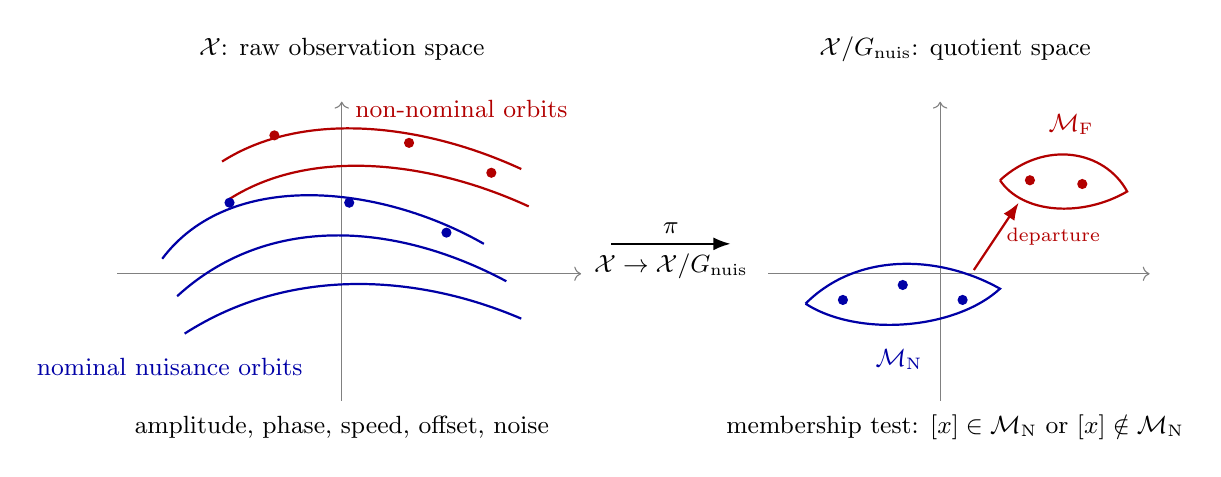
\begin{tikzpicture}[
    scale=0.95,
    every node/.style={font=\small},
    orbit/.style={thick},
    point/.style={circle, fill, inner sep=1.3pt},
    arrow/.style={-{Latex[length=2.2mm]}, thick},
    manifold/.style={thick}
]
% ---- left panel: raw observation space ----
\node at (0,3.0) {\(\X\): raw observation space};
\draw[->, gray] (-3,0) -- (3.2,0);
\draw[->, gray] (0,-1.7) -- (0,2.3);

\draw[orbit, blue!65!black] (-2.4,0.2) .. controls (-1.5,1.4) and (0.5,1.2) .. (1.9,0.4);
\draw[orbit, blue!65!black] (-2.2,-0.3) .. controls (-1.0,0.8) and (0.7,0.7) .. (2.2,-0.1);
\draw[orbit, blue!65!black] (-2.1,-0.8) .. controls (-0.7,0.1) and (1.0,0.0) .. (2.4,-0.6);
\draw[orbit, red!70!black] (-1.6,1.5) .. controls (-0.5,2.2) and (1.1,2.0) .. (2.4,1.4);
\draw[orbit, red!70!black] (-1.5,1.0) .. controls (-0.4,1.7) and (1.2,1.5) .. (2.5,0.9);

\node[point, blue!65!black] at (-1.5,0.95) {};
\node[point, blue!65!black] at (0.1,0.95) {};
\node[point, blue!65!black] at (1.4,0.55) {};
\node[point, red!70!black] at (-0.9,1.85) {};
\node[point, red!70!black] at (0.9,1.75) {};
\node[point, red!70!black] at (2.0,1.35) {};

\node[blue!65!black] at (-2.3,-1.25) {nominal nuisance orbits};
\node[red!70!black] at (1.6,2.2) {non-nominal orbits};
\node at (0,-2.05) {amplitude, phase, speed, offset, noise};

% ---- projection ----
\draw[arrow] (3.6,0.4) -- (5.2,0.4)
  node[midway, above] {\(\pi\)}
  node[midway, below] {\(\X \to \quotient\)};

% ---- right panel: quotient space ----
\node at (8.2,3.0) {\(\quotient\): quotient space};
\draw[->, gray] (5.7,0) -- (10.8,0);
\draw[->, gray] (8.0,-1.7) -- (8.0,2.3);

\draw[manifold, blue!65!black]
    (6.2,-0.4) .. controls (6.9,0.3) and (8.0,0.25) .. (8.8,-0.2)
    .. controls (8.2,-0.75) and (6.9,-0.85) .. (6.2,-0.4);
\node[blue!65!black] at (7.45,-1.15) {\(\Mnominal\)};

\draw[manifold, red!70!black]
    (8.8,1.25) .. controls (9.4,1.8) and (10.2,1.65) .. (10.5,1.1)
    .. controls (9.9,0.75) and (9.1,0.8) .. (8.8,1.25);
\node[red!70!black] at (9.75,2.0) {\(\Mfault\)};

\node[point, blue!65!black] at (6.7,-0.35) {};
\node[point, blue!65!black] at (7.5,-0.15) {};
\node[point, blue!65!black] at (8.3,-0.35) {};
\node[point, red!70!black] at (9.2,1.25) {};
\node[point, red!70!black] at (9.9,1.2) {};

\draw[arrow, red!70!black] (8.45,0.05) -- (9.05,0.95)
  node[midway, right] {\scriptsize departure};

\node[align=center] at (8.2,-2.05) {%
membership test: \([x]\in\Mnominal\) or \([x]\notin\Mnominal\)};
\end{tikzpicture}
\caption{Functional manifolds as quotient geometry. In raw observation space,
nuisance transformations generate extended orbits of observations that share
the same latent physical state. The quotient projection \(\pi\) collapses
those orbits into equivalence classes, exposing compact nominal and
non-nominal functional regions. Diagnosis is then a membership test in
\(\Mnominal\) rather than a partition of labelled observations.}
\label{fig:quotient_manifold_concept}
\end{figure}

This also clarifies the relation between anomaly detection and
classification. A supervised classifier learns a partition of labelled
observations. A quotient-space diagnostic operator learns a representation in
which physically equivalent observations are identified. Operational labels
may subsequently be attached to the recovered regions, but the regions precede
the labels; that is the subject of
Section~\ref{sec:emergent_classification}.

%---------------------------------------------------------------------
\subsection{The saturation radius}
\label{subsec:saturation_radius}
%---------------------------------------------------------------------

The companion report \citep{disanti2026inverse} proposes that a regime becomes
learnable when its geometric descriptors stabilize under additional
observations, written informally as
\begin{equation}
H(n)\to H^*,\qquad
r_{\max}(n)\to r^*,\qquad
V(n)\to V^*,
\label{eq:saturation_informal}
\end{equation}
for an entropy, a radius and a volume descriptor. As stated,
\eqref{eq:saturation_informal} is a description of observed behaviour rather
than a claim with a definite content: neither the estimators nor the mode of
convergence is specified. We therefore fix one descriptor precisely, the
radius, and show that doing so brings saturation within reach of the same
machinery used in Section~\ref{sec:computational_realization}.

Let \(\phi:\X\to\Z\) be a representation map and let \(\nu\) denote the law
induced on \(\Z\) by drawing \(\eta\) from the nominal nuisance law and
applying \(\phi\circ F(\theta_{\mathrm N},\cdot)\). Fix a reference point
\(c\in\Z\), for instance the mean of \(\nu\), and define the scalar
\begin{equation}
D = d\bigl(\phi(x),c\bigr), \qquad x = F(\theta_{\mathrm N},\eta),
\label{eq:radial_variable}
\end{equation}
with distribution function \(F_D\).

\begin{definition}[Population and empirical saturation radius]
\label{def:saturation_radius}
For \(p\in(0,1)\) the \emph{population \(p\)-radius} of the nominal regime is
the quantile
\begin{equation}
R_p = F_D^{-1}(p) = \inf\{r\ge 0 : F_D(r)\ge p\},
\label{eq:population_radius}
\end{equation}
and given \(n\) nominal observations with radial values
\(D_1,\ldots,D_n\) the \emph{empirical \(p\)-radius} \(\widehat R_p(n)\) is the
corresponding empirical quantile. The descriptor \(r_{\max}(n)\) of
\eqref{eq:saturation_informal} is the case \(p\to 1\), and the \(p_{95}\) and
\(p_{98}\) radii used in the companion work are the cases \(p=0.95\) and
\(p=0.98\).
\end{definition}

The first thing this definition buys is that the object being estimated exists
and is finite, which does not follow from \eqref{eq:saturation_informal} on its
own but does follow from Section~\ref{sec:quotient_formulation}.

\begin{corollary}[Finiteness of the saturation radius]
\label{cor:finite_radius}
Under Assumption~\ref{ass:compact_eta}, if \(\phi\) is continuous then \(D\) is
a bounded random variable and \(R_p<\infty\) for every \(p\in(0,1)\); moreover
\(\sup_{\eta\in\EtaSpace} D<\infty\), so the regime has a finite radius in the
Hausdorff sense.
\end{corollary}

\begin{proof}
By Proposition~\ref{prop:compactness} the closure
\(\overline{\mathcal{O}_{\mathrm N}}\) is compact, and \(\phi\) is continuous,
so \(\phi(\overline{\mathcal{O}_{\mathrm N}})\) is compact in \(\Z\). The map
\(z\mapsto d(z,c)\) is continuous, and a continuous real function on a compact
set is bounded and attains its supremum. Hence \(D\) is bounded and every
quantile of \(F_D\) is finite.
\end{proof}

Corollary~\ref{cor:finite_radius} is the precise sense in which the compactness
result of Section~\ref{sec:quotient_formulation} underwrites the
finite-Hausdorff-radius premise of the functional-topological foundation
discussed in Remark~\ref{rem:blueprints_relation}. Saturation can then be
stated as a convergence claim about an estimator of a finite quantity.

\begin{proposition}[Consistency of the empirical saturation radius]
\label{prop:radius_consistency}
Let \(D_1,D_2,\ldots\) be independent draws of \eqref{eq:radial_variable} and
suppose \(F_D\) is strictly increasing in a neighbourhood of \(R_p\), so that
the quantile is unique. Then
\begin{equation}
\widehat R_p(n) \longrightarrow R_p \qquad \text{almost surely as } n\to\infty .
\label{eq:radius_consistency}
\end{equation}
\end{proposition}

\begin{proof}
By the Glivenko--Cantelli theorem the empirical distribution function
converges to \(F_D\) uniformly and almost surely. Uniqueness of the quantile at
level \(p\) transfers uniform convergence of the distribution function to
pointwise convergence of the quantile function at \(p\); see, for example,
\citet[Sec.~2.3]{serfling1980} or \citet[Lemma~21.2]{vandervaart1998}.
\end{proof}

Proposition~\ref{prop:radius_consistency} makes
\eqref{eq:saturation_informal} a theorem rather than an observation, and it
identifies the limit as a specific population quantile. It is, however, purely
asymptotic, and therefore silent on the question the operational criterion
actually poses, namely how many observations suffice.

%---------------------------------------------------------------------
\subsection{Finite-sample certification of saturation}
\label{subsec:saturation_certification}
%---------------------------------------------------------------------

That question is answered by the argument of
Section~\ref{subsec:distribution_free}. % Definition~\ref{def:saturation_radius}
makes the saturation radius a quantile of a nominal distribution estimated from
finitely many samples, which is exactly what the local operational radius is;
only the space differs, distances in \(\Z\) rather than residuals in \(\R\).
Proposition~\ref{prop:coverage} is stated for an arbitrary exchangeable scalar
sequence and therefore applies unchanged.

We note the forward dependency explicitly. Proposition~\ref{prop:coverage} is
proved in Section~\ref{subsec:distribution_free} rather than here because its
operational role is the calibration of the decision boundary, which is where a
reader will expect to find it; but it is a statement about exchangeable
real-valued sequences and is logically independent of everything specific to
residuals, as recorded in Remark~\ref{rem:saturation_link}. The corollary below
therefore borrows a later result without circularity.

\begin{corollary}[Distribution-free certification of the saturation radius]
\label{cor:saturation_certification}
Let \(D_1,\ldots,D_n,D_{n+1}\) be exchangeable with an atomless marginal, let
\(\alpha=1-p\), and set
\begin{equation}
\widehat R^{\,\star}_p = D_{(k_\alpha)},
\qquad k_\alpha = \bigl\lceil p\,(n+1) \bigr\rceil .
\label{eq:radius_order_statistic}
\end{equation}
Then, provided \(n\ge 1/\alpha-1\),
\begin{equation}
p \;\le\; \Prob\bigl(D_{n+1}\le \widehat R^{\,\star}_p\bigr)
  \;=\; \frac{k_\alpha}{n+1}
  \;\le\; p+\frac{1}{n+1},
\label{eq:radius_coverage}
\end{equation}
and \(\widehat R^{\,\star}_p\) equals the largest observed radial value
\(D_{(n)}\) precisely when \(1/\alpha-1\le n<2/\alpha-1\).
\end{corollary}

\begin{proof}
Apply Proposition~\ref{prop:coverage}, Corollary~\ref{cor:min_commissioning}
and Corollary~\ref{cor:degenerate_range} with \(\residual_i\) replaced by
\(D_i\). Neither the coverage argument nor the two corollaries uses any
property of the scalar sequence beyond exchangeability and atomlessness.
\end{proof}

Corollary~\ref{cor:saturation_certification} unifies the two halves of the
framework, and its practical content is the same in both. Certifying that a
regime's empirical extent covers a fraction \(p\) of its nominal orbit
requires at least \(1/\alpha-1\) observations, so \(49\) at \(p=0.98\); and
because the certified radius is the observed maximum throughout
\(1/\alpha-1\le n<2/\alpha-1\), a saturation curve that appears to have
levelled off anywhere in that band has levelled off at the most variable
statistic available, which is a property of the estimator rather than evidence
about the regime. For \(p=0.98\) a non-degenerate saturation radius requires
\(n\ge 99\).

\begin{remark}[Plug-in reference points break exchangeability]
\label{rem:plugin_centroid}
The radial variable \eqref{eq:radial_variable} is defined against a fixed
reference \(c\). In practice \(c\) is estimated from data, and the companion
work additionally estimates the projection in which distances are measured
from the same sample. Both substitutions make \(D_1,\ldots,D_n\) depend on one
another and destroy the exchangeability of the augmented sequence, so
Corollary~\ref{cor:saturation_certification} then holds only approximately,
with an error that vanishes as the reference is estimated more precisely. The
remedy is the same split-sample construction available in
Remark~\ref{rem:optional_stopping}: estimate the reference point, and the
projection if one is used, on a block of nominal observations disjoint from the
block used to compute the radius. This restores exchangeability by
construction and costs only observations, not assumptions.
\end{remark}

\begin{remark}[What a saturation curve does and does not establish]
\label{rem:saturation_semantics}
Observed flattening of \(\widehat R_p(n)\) is a stopping heuristic, not a
proof that \(R_p\) has been recovered, exactly as convergence of the
commissioning criterion is not a proof that the population residual quantile
has been recovered (Remark~\ref{rem:stopping_semantics}). An upper quantile
estimated from few upper-tail observations can remain flat over an interval and
then move again when a further extreme nominal observation arrives, and
Corollary~\ref{cor:saturation_certification} says nothing to the contrary: it
bounds coverage at a given \(n\), not the increments of the curve. Claims of
the form ``the geometry has stabilized by \(n\approx 500\)'' should therefore be
read as descriptions of the observed trajectory, with the coverage statement
supplying the part that is guaranteed.
\end{remark}

\begin{remark}[The saturation curve and the guarantee pull in opposite directions]
\label{rem:saturation_tension}
The measurements reported in Section~\ref{sec:results} sharpen
Remark~\ref{rem:saturation_semantics} into a concrete warning about the
estimator, and the effect is not small. Inside the degenerate range the
certified radius \emph{is} the sample maximum, so it drifts systematically
upward with \(n\): on simulated nominal data at \(p=0.98\) its mean rises from
about \(2\%\) above \(R_p\) at \(n=49\) to about \(6\%\) above at \(n=98\), and
then falls discontinuously at \(n=99\), where an interior order statistic first
becomes available. A saturation curve computed with the certified estimator
therefore \emph{cannot} flatten inside the band; apparent settling there is the
maximum of a growing sample.

The interpolated estimator behaves in exactly the complementary way. It
produces the familiar smooth curve approaching \(R_p\) from below, and it
undercovers at every sample size examined. The reassuring visual and the
coverage guarantee are thus in tension: the estimator that makes a saturation
plot look convergent is precisely the one that fails to certify, and the
estimator that certifies does not produce a flat curve until the degenerate
range has been left behind. Saturation should accordingly be reported with the
attained coverage alongside the curve, and with \(n\ge 2/\alpha-1\).
\end{remark}

\begin{remark}[The saturation radius is a diagnostic, not a detector]
\label{rem:radius_not_detector}
One further empirical observation limits what a saturation analysis can be
asked to show. Measuring the certified radius of each simulated regime under a
shared two-dimensional nominal projection separates them barely at all: the
ratios of fault to nominal radius are between \(0.98\) and \(1.04\), that is, no
separation. The reason is mechanical. A low-dimensional principal projection of
a raw vibration window is dominated by the shaft harmonics, whereas the fault
signature is a low-amplitude impulse train contributing almost nothing to the
leading variance directions. The same simulator, the same nominal-only fitting
and the same membership rule yield \(99\)--\(100\%\) detection when membership
is tested through a reconstruction residual instead
(Section~\ref{sec:results}).

Two consequences follow. First, a saturation plot is evidence about the
sampling of the nominal geometry, not about regime separability, and should not
be cited for the latter. Second, this is the empirical reason the framework
poses diagnosis through a residual, as in
Section~\ref{sec:computational_realization}, rather than through a radius in a
projection: Assumption~\ref{ass:residual_proxy} asks the score to track
distance to the nominal manifold, and a leading-variance radius demonstrably
does not.
\end{remark}

% ============================================================================
\section{Emergent Classification via Expert Feedback}
\label{sec:emergent_classification}
% [MERGE: COMPANION "Emergent Classification Through Expert Feedback" and
% "Consequences for Classification"] + [NEW: per-class coverage corollary,
% set-valued formulation, and an explicit separation-versus-coverage scope
% statement grounded in the Experiment 6 negative result]. WRITTEN.

Sections~\ref{sec:quotient_formulation}--\ref{sec:manifolds_saturation}
concern a single regime: the nominal one. This section states what the same
construction gives when several regimes have been recovered, which is the
point at which the framework makes contact with classification. The answer is
deliberately asymmetric: the geometry supplies a great deal about when a class
should \emph{not} be rejected, and very little about when a competing class
should be, and that asymmetry is the substance of the section.

%---------------------------------------------------------------------
\subsection{Two levels of classification}
\label{subsec:two_levels}
%---------------------------------------------------------------------

Classification in this framework occurs at two levels, and conflating them is
the source of most of the confusion the inverse-problem view is meant to
dispel.

The first is \emph{structural} classification. A new observation is assigned
to a recovered functional region, to an emerging region that has not yet
saturated, to a transition between regions, or to none of them. This
assignment requires no semantic labels at all: it is induced by the geometry
of the quotient space and by the membership test \eqref{eq:membership}.

The second is \emph{operational} classification. Once a region has stabilized
in the sense of Section~\ref{sec:manifolds_saturation}, an expert or a
downstream policy may attach meaning to it: normal operation, harmless
variation, friction, heat, degradation, or a known fault regime. Classification
is therefore not absent before labels exist; it first appears as geometric
membership and only later becomes semantic.

%---------------------------------------------------------------------
\subsection{Manifold-level labelling}
\label{subsec:manifold_labelling}
%---------------------------------------------------------------------

Let \(\{\mathcal{M}_j\}_{j=1}^{k}\) denote a family of recovered compact
regions in \(\quotient\), of which \(\Mnominal\) is one. Labels are attached
at the level of regions rather than of samples, through a map
\begin{equation}
L:\{\mathcal{M}_j\}_{j=1}^{k}\longrightarrow \mathcal{Y},
\qquad L(\mathcal{M}_j)=y_j .
\label{eq:labelling_map}
\end{equation}
The contrast with supervised practice is the object being labelled. A
supervised classifier consumes \(x_i\mapsto y_i\) over many individual
samples; here the expert supplies \(\mathcal{M}_j\mapsto y_j\), once per
recovered region. The labelling effort is proportional to the number of
regimes, not to the number of observations.

Given a residual \(\residual_j\) for each region, in the sense of
Assumption~\ref{ass:residual_proxy}, and a radius \(\tau_j\) calibrated for
that region by Proposition~\ref{prop:coverage}, the admissible set for an
observation is
\begin{equation}
\Gamma(x) \;=\; \bigl\{\, j \in \{1,\ldots,k\} \;:\; \residual_j(x)\le\tau_j \,\bigr\},
\label{eq:admissible_set}
\end{equation}
and the reported diagnosis is
\begin{equation}
\hat y(x)=
\begin{cases}
L(\mathcal{M}_j), & \Gamma(x)=\{j\},\\[2pt]
\{L(\mathcal{M}_j)\}_{j\in\Gamma(x)}, & |\Gamma(x)|>1 \quad\text{(ambiguous)},\\[2pt]
\mathrm{unknown}, & \Gamma(x)=\emptyset .
\end{cases}
\label{eq:set_valued_rule}
\end{equation}

Writing the rule as a set rather than an \(\arg\min\) is not a stylistic
choice. It is what the calibration of
Section~\ref{sec:computational_realization} actually licenses, and it makes
the two failure modes explicit rather than hiding them behind a nearest-region
assignment: an observation may satisfy no region, which is the abstention
\eqref{eq:membership} already anticipates, or it may satisfy several. The
construction is the class-conditional, or Mondrian, form of a conformal
predictor \citep{vovk2005,shafer2008}, arrived at here from the quotient
geometry rather than imported.

\begin{corollary}[Per-class non-rejection]
\label{cor:per_class_coverage}
Fix a region \(\mathcal{M}_j\) and suppose the residuals
\(\residual_j\) evaluated on observations from regime \(j\) satisfy
Assumption~\ref{ass:exchangeability}, with \(\tau_j\) calibrated from
\(n_j\ge 1/\alpha_j-1\) such observations by
\eqref{eq:radius_order_statistic}. Then for a further observation \(x\) drawn
from regime \(j\),
\begin{equation}
\Prob\bigl(j\in\Gamma(x)\bigr)\;\ge\;1-\alpha_j .
\label{eq:per_class_coverage}
\end{equation}
Consequently the true regime is retained in the admissible set with
probability at least \(1-\alpha_j\), simultaneously for every regime, without
any assumption on the residual distributions and without any calibration data
from competing regimes.
\end{corollary}

\begin{proof}
Apply Proposition~\ref{prop:coverage} to the exchangeable sequence generated
by \(\residual_j\) on regime \(j\); the event \(\{j\in\Gamma(x)\}\) is
precisely \(\{\residual_j(x)\le\tau_j\}\). The statement is per-regime and the
regimes are calibrated independently, so no joint assumption is required.
\end{proof}

Corollary~\ref{cor:per_class_coverage} formalizes what the framework buys.
Each region is calibrated only against its own nominal behaviour, so a new
regime can be added after deployment without recalibrating the others, and a
regime for which no data yet exists simply contributes nothing to
\(\Gamma(x)\). This is the sense in which the taxonomy may grow: adding
\(\mathcal{M}_{k+1}\) changes \eqref{eq:admissible_set} by one term and leaves
\eqref{eq:per_class_coverage} untouched for \(j\le k\).

Several structural consequences follow, and they are the ones the companion
report anticipates informally \citep{disanti2026inverse}: two regions may
carry the same label when they are operational variants of one regime; a
single nominal label may resolve into several regions when the underlying
behaviour is heterogeneous; an unfamiliar observation need not be forced into
the nearest known class; and expert effort attaches to regions rather than to
samples.

%---------------------------------------------------------------------
\subsection{What coverage does not give: separation}
\label{subsec:coverage_not_separation}
%---------------------------------------------------------------------

Corollary~\ref{cor:per_class_coverage} bounds the probability of wrongly
\emph{excluding} the true regime. It says nothing whatever about wrongly
\emph{including} a competing one, and the distinction is not a technicality.

\begin{remark}[Coverage is not discrimination]
\label{rem:coverage_not_discrimination}
Nothing in \eqref{eq:per_class_coverage} prevents
\(|\Gamma(x)|>1\). The acceptance regions \(\{\residual_j\le\tau_j\}\) are
calibrated independently and may overlap arbitrarily; in the extreme, if two
regions are geometrically indistinguishable under the available residuals,
every observation from either is admitted by both, and
\eqref{eq:per_class_coverage} still holds exactly. A guarantee about
non-rejection is therefore compatible with a diagnosis that is always
ambiguous. Reducing \(|\Gamma(x)|\) requires \emph{separation} between
regions, which is a property of the representation and must be established
separately; it does not follow from the quotient construction of
Section~\ref{sec:quotient_formulation}, from compactness, or from any
calibration argument.
\end{remark}

\begin{remark}[Two obstructions visible in the present construction]
\label{rem:classification_obstructions}
The computational realization of
Section~\ref{sec:computational_realization} does not by itself supply that
separation, for two distinct reasons, and the experiments of
Section~\ref{sec:results} exhibit both.

First, a scalar residual is a many-to-one map. The rule
\eqref{eq:decision_rule} tests departure from the nominal region and reports a
single number, from which the \emph{direction} of departure cannot be
recovered. Detection of a fault and identification of its type are therefore
not the same problem in this construction, and the second requires \(k\)
residuals, one per region, each with its own representation and its own
calibration, not one residual with \(k\) thresholds.

Second, the low-dimensional radial diagnostic of
Section~\ref{sec:manifolds_saturation} does not separate the regimes it
describes. Measured on simulated data under a shared two-dimensional nominal
projection, the ratio of fault radius to nominal radius lies between \(0.98\)
and \(1.04\) (Section~\ref{sec:results}), that is, no separation at all, even
though the same simulator and the same nominal-only fitting give
\(99\)--\(100\%\) detection through the reconstruction residual. Saturation of
a region and separability of that region from its neighbours are independent
properties, and evidence for the former is not evidence for the latter.
\end{remark}

This is the precise sense in which fault classification remains open in the
present work, and it locates the gap left by the companion technical note
\citep{disanti2026quotient} rather than closing it. What has been established
is that diagnosis factors through the quotient
(Proposition~\ref{prop:quotient_diagnosis}), so a correct classifier exists as
a function of \([x]\) alone; that regions, once recovered, can be labelled and
calibrated individually with distribution-free per-class validity
(Corollary~\ref{cor:per_class_coverage}); and that abstention and ambiguity
are reported rather than concealed \eqref{eq:set_valued_rule}. What has not
been established is that any particular representation renders the non-nominal
regions separable. Section~\ref{sec:future_work} records the experiment that
would test it.

% ============================================================================
\section{Computational Realization and Local Calibration}
\label{sec:computational_realization}
% [MERGE: TECHNOTE Sec.6 + TRB Sec.3 Method] + [NEW: Prop. 3, Cor. 3,
% Remarks 5-9]. WRITTEN.

Sections~\ref{sec:observation_model}--\ref{sec:emergent_classification}
characterize the diagnostic object: a compact, connected nominal region
\(\Mnominal\) in a quotient space, with anomaly defined as failure of
membership in that region. That characterization is not yet an algorithm.
Two quantities must be supplied before
\eqref{eq:membership} can be evaluated on data: a computable surrogate for
distance to \(\Mnominal\), and a decision boundary on that surrogate.

This section supplies both. Section~\ref{subsec:representation_operator}
introduces the representation operator and the residual used as a distance
surrogate. Section~\ref{subsec:scale_transfer} explains, as a consequence
of Proposition~\ref{prop:quotient_diagnosis}, why the representation is
transferable across assets while the numerical scale of the residual is
not, which is the structural reason a single global decision boundary
cannot be used. Sections~\ref{subsec:mc_calibration} and
\ref{subsec:distribution_free} then give the calibration procedure and its
guarantee: the central new result,
Proposition~\ref{prop:coverage}, shows that a radius chosen as an
appropriate order statistic of nominal commissioning residuals attains a
prescribed coverage level without any assumption on the residual
distribution, and Corollary~\ref{cor:min_commissioning} converts this into
a minimum commissioning length.

Throughout this section we index physical assets, or more generally
independently commissioned monitoring environments, by \(k\).

%---------------------------------------------------------------------
\subsection{Representation operator and diagnostic residual}
\label{subsec:representation_operator}
%---------------------------------------------------------------------

Let \(E:\X\rightarrow\Z\) be an encoder and \(D:\Z\rightarrow\X\) a
decoder, with reconstruction
\begin{equation}
\hat{x} = D(E(x)),
\label{eq:reconstruction}
\end{equation}
and define the \emph{diagnostic residual}
\begin{equation}
\residual(x) = \frac{1}{n_w}\bigl\|x-\hat{x}\bigr\|_2^2 .
\label{eq:residual}
\end{equation}
In the present realization \(E\) and \(D\) are the encoder and decoder of a
one-dimensional convolutional autoencoder trained exclusively on nominal
windows generated by Monte Carlo sampling of \(\EtaSpace\); autoencoders
have long been used both as nonlinear representation learners
\citep{hinton2006} and as reconstruction-based anomaly detectors
\citep{sakurada2014}. No non-nominal observation is used at any stage of
representation learning.

\begin{assumption}[Residual--distance proxy]
\label{ass:residual_proxy}
The diagnostic residual \(\residual(x)\) is treated as a computable proxy
that is monotonically related to distance to the nominal quotient manifold:
\begin{equation}
\residual(x) \;\approx\; d\bigl([x],\Mnominal\bigr).
\label{eq:distance_proxy}
\end{equation}
\end{assumption}

Assumption~\ref{ass:residual_proxy} is an operational hypothesis, not a
consequence of the training objective. Minimizing mean-squared
reconstruction error on nominal data does not by itself guarantee that
\(\residual\) is isometric, or even monotonic, with respect to any
particular metric on \(\quotient\). The assumption is therefore evaluated
empirically in Section~\ref{sec:results}, where the separation between
nominal and non-nominal residual distributions is the relevant evidence,
and it is listed among the limitations in
Section~\ref{sec:limitations}.

The substantive claim is not that mean-squared error is the correct
residual. It is that a residual can serve as an operational test for
membership in the nominal quotient manifold. Any score with the qualitative
property in \eqref{eq:distance_proxy} may be substituted: a latent
likelihood, a Mahalanobis distance in \(\Z\), an energy score, a diffusion
or denoising score, a predictive error, or a physics-informed residual. The
calibration theory of
Section~\ref{subsec:distribution_free} is stated for an arbitrary residual
and is therefore unaffected by that choice.

%---------------------------------------------------------------------
\subsection{Why the representation transfers but its scale does not}
\label{subsec:scale_transfer}
%---------------------------------------------------------------------

Proposition~\ref{prop:quotient_diagnosis} states that the ideal diagnostic
map factors through the quotient. Write that ideal map as the membership
predicate
\begin{equation}
h(x) = \indicator\bigl[\,[x]\notin\Mnominal\,\bigr],
\label{eq:ideal_predicate}
\end{equation}
so that \(h=\bar h\circ\pi\) by Proposition~\ref{prop:quotient_diagnosis},
and \(h\) is constant on nuisance orbits. The computable surrogate actually
evaluated on data is
\begin{equation}
h_\tau(x) = \indicator\bigl[\,\residual(x) > \tau\,\bigr].
\label{eq:surrogate_predicate}
\end{equation}

\begin{remark}[Invariance is inherited by the predicate, not by the score]
\label{rem:scale_not_invariant}
The surrogate \eqref{eq:surrogate_predicate} does not inherit the
orbit-invariance of \eqref{eq:ideal_predicate}. The residual
\(\residual\) is a function on \(\X\), not on \(\quotient\): it is not
\(\Gnuis\)-invariant, because the reconstruction error attained by a fixed
pair \((E,D)\) varies over an orbit even when the latent state does not.
Consequently, for a fixed \(\tau\) the level set
\(\{\residual = \tau\}\) is not the \(\pi\)-preimage of a subset of the
quotient, and \(h_\tau\) is not constant on orbits. What the quotient
structure does guarantee, via
Proposition~\ref{prop:quotient_diagnosis}, is that a \emph{correct}
diagnostic decision exists as a function of \([x]\) alone. Recovering it
from \(\residual\) requires choosing \(\tau\) so that the level set
approximates \(\partial\Mnominal\) under the nuisance law actually realized
by the asset being monitored.
\end{remark}

Remark~\ref{rem:scale_not_invariant} has a direct architectural
consequence, and it is the reason the calibration problem is posed
per-asset rather than globally. The representation \((E,D)\) encodes which
directions of variation are nuisance and which are diagnostic; that
information is a property of the asset family and is transferable. The
numerical value of \(\residual\) additionally reflects the sensor coupling,
mounting, operating point, preprocessing, and the particular optimization
trajectory that produced \((E,D)\); none of that is transferable. We
therefore adopt the following separation:

\begin{itemize}[leftmargin=1.5em]
\item one representation operator, learned once from simulated nominal
observations and thereafter held fixed;
\item one scalar \emph{local operational radius} \(\tau_k^\star\) per
monitored asset, estimated from that asset's own nominal observations.
\end{itemize}

The decision rule for asset \(k\) at time \(t\) is then
\begin{equation}
\hat y\bigl(x_{k,t}\bigr) =
\begin{cases}
\text{anomalous}, & \residual(x_{k,t}) > \tau_k^\star,\\[2pt]
\text{nominal},   & \residual(x_{k,t}) \le \tau_k^\star .
\end{cases}
\label{eq:decision_rule}
\end{equation}

This prediction is falsifiable and is tested directly in
Section~\ref{sec:results}: transferring the residual \emph{scale} across
the simulation-to-field boundary should fail, while transferring the
representation and re-estimating only \(\tau_k^\star\) should not.

%---------------------------------------------------------------------
\subsection{Monte Carlo reference calibration}
\label{subsec:mc_calibration}
%---------------------------------------------------------------------

A reference boundary can be computed entirely in simulation. Let
\(\mu_{\mathrm{MC}}\) and \(\sigma_{\mathrm{MC}}\) denote the mean and
standard deviation of \(\residual\) over held-out nominal Monte Carlo
windows, and let \(q\in(0,1)\) denote a target nominal coverage level. A
parametric reference is
\begin{equation}
\taumc(q) = \mu_{\mathrm{MC}} + z_q\,\sigma_{\mathrm{MC}},
\label{eq:tau_mc_quantile}
\end{equation}
with \(z_q\) the corresponding standard-normal quantile; alternatively
\(\taumc(q)\) may be taken as the empirical \(q\)-quantile of the synthetic
nominal residual distribution.

The level \(q\) is not part of the mathematical formulation. It is an
operational risk parameter: lower values increase sensitivity at the cost of
false alarms, higher values reduce false alarms at the cost of delayed
detection of weak or incipient deviations.

\begin{remark}[\(\taumc\) is a reference, not a deployable radius]
\label{rem:mc_not_deployable}
By Remark~\ref{rem:scale_not_invariant}, \(\taumc(q)\) calibrates the
residual scale of the \emph{simulator}, not of any physical asset. It is
reported here because it is the natural baseline and because its failure is
informative, not because it is proposed as an operating point. The
corresponding experiment is the direct-transfer condition of
Section~\ref{sec:results}.
\end{remark}

%---------------------------------------------------------------------
\subsection{Distribution-free calibration of the local operational radius}
\label{subsec:distribution_free}
%---------------------------------------------------------------------

We now give the calibration procedure a guarantee. Before doing so it is
worth being explicit about what is being estimated, because the scalar form
of \(\tau_k^\star\) invites a misreading.

\begin{remark}[A set is being estimated, not a threshold tuned]
\label{rem:support_estimation}
The decision rule \eqref{eq:decision_rule} compares a scalar to a scalar, but
the object it defines is the region
\begin{equation}
\widehat{S}_k \;=\; \bigl\{\, x\in\X \;:\; \residual(x)\le\tau_k^\star \,\bigr\},
\label{eq:acceptance_region}
\end{equation}
a level set of the residual, and the guarantee below is a statement about the
nominal probability mass that \(\widehat{S}_k\) contains. The task is
therefore \emph{support estimation} rather than threshold calibration: no
trade-off between error types is being tuned, and no fault data is consulted
to place the boundary. This is the problem posed by
\citet{devroye1980}, who introduced support estimation precisely in order to
decide whether a new measurement belongs to the support of a distribution
observed so far, and it is the problem the one-class formulation of
\citet{scholkopf2001} and the minimum-volume-set literature
\citep{scott2006} address with different estimators.

The distinction matters for how the framework should be judged. A tuned
threshold is answerable to the error rates it achieves on labelled faults; an
estimated region with prescribed nominal coverage is answerable to whether it
attains that coverage, which can be checked without any fault observation
whatsoever. The residual supplies the family of candidate regions, indexed by
\(\tau\); Section~\ref{sec:quotient_formulation} supplies the reason a
bounded region exists to be estimated
(Corollary~\ref{cor:bounded_manifold}) and the reason its boundary is a
well-defined object in the quotient
(Proposition~\ref{prop:boundary_invariant}); and the argument below selects a
member of the family with a distribution-free coverage property.
\end{remark}

\begin{remark}[A level is estimated, not a shape]
\label{rem:level_not_shape}
The previous remark should not be read as a stronger claim than it is. The
calibration selects one member of the one-parameter family
\(\{\,\residual\le\tau\,\}_{\tau>0}\); the \emph{shape} of that region is
fixed entirely by \(\residual\) and is not estimated at all. Different
residuals induce quite different geometries for the same nominal data: a
reconstruction error against a linear subspace yields regions elongated along
the retained directions, a Mahalanobis distance yields ellipsoids, a
nearest-neighbour distance yields unions of balls in the manner of
\citet{devroye1980}, and a kernel one-class construction
\citep{scholkopf2001} or a nonlinear autoencoder yields level sets with no
closed-form description. Proposition~\ref{prop:coverage} is indifferent
between them: each attains the stated coverage, and coverage alone cannot
distinguish a well-shaped region from a badly shaped one, exactly as
Remark~\ref{rem:coverage_not_discrimination} observes for the multi-region
case.

That shape is consequential rather than cosmetic is not a conjecture here.
Section~\ref{sec:results} reports that a radius in a two-dimensional
projection, whose acceptance region is a ball, fails to separate the fault
regimes at all, while the reconstruction residual computed from the same
nominal data under the same calibration separates them at
\(79\)--\(100\%\). The nominal coverage is the same in both cases; only the
geometry of the accepted region differs.

The honest position is therefore that this work certifies the level and
inherits the shape. Estimating the shape is the province of minimum-volume-set
estimation \citep{scott2006} and of the support-estimation constructions cited
above, which choose the region rather than a level within a fixed family, and
combining such an estimator with the distribution-free calibration used here
is a natural continuation recorded in Section~\ref{sec:future_work}.
\end{remark}

Before calibrating anything it is worth asking whether the object being
estimated exists at all. It does, and for purely topological reasons.

\begin{proposition}[Existence of a finite nominal radius]
\label{prop:finite_nominal_radius}
Assume the hypotheses of Proposition~\ref{prop:compactness}, and let the
representation \(\phi\) and the residual \(\residual\) be continuous. Then
\begin{enumerate}[label=(\roman*),leftmargin=1.8em]
\item \(\phi\bigl(\overline{\mathcal{O}_{\mathrm N}}\bigr)\) is compact in
      \(\Z\);
\item the acceptance region \(\widehat{S}=\{\residual\le\tau\}\) is closed in
      \(\X\) for every \(\tau\); and
\item \(\residual\) attains a finite maximum
      \(\residual^{*}=\max_{x\in\overline{\mathcal{O}_{\mathrm N}}}\residual(x)\),
      so that \(\{\residual\le\residual^{*}\}\supseteq
      \overline{\mathcal{O}_{\mathrm N}}\).
\end{enumerate}
\end{proposition}

\begin{proof}
(i) A continuous image of a compact set is compact
\citep[Thm.~4.14]{rudin1976}. (ii) \(\widehat{S}=\residual^{-1}
\bigl((-\infty,\tau]\bigr)\) is the preimage of a closed set under a
continuous map, hence closed. (iii) A continuous real-valued function on a
compact set attains its supremum \citep[Thm.~4.16]{rudin1976}; the inclusion
is immediate from the definition of the maximum.
\end{proof}

Part (iii) is the exact, noise-free counterpart of the statistical radius: a
single finite level suffices to accept the entire nominal orbit, with no
exceptions. It is the topological content of the premise that physically
generated signals do not vary without bound, and it is stronger than
Corollary~\ref{cor:finite_radius}, which asserts finiteness only for
\(p\in(0,1)\).

Two objections to Proposition~\ref{prop:finite_nominal_radius} suggest
themselves, and both can be answered at the cost of an additional and
physically mild assumption. A third cannot, and survives.

The first objection is that \(\residual^{*}\) is a supremum over a set never
observed in full, so that any finite sample yields a maximum over a subset and
underestimates it. This is true but quantitatively harmless, because the set
in question is compact and of low dimension.

\begin{proposition}[The sample maximum approximates the true maximum]
\label{prop:fill_distance}
Let \(K\subset\X\) be compact, let \(\residual\) be Lipschitz on \(K\) with
constant \(L\), and let \(x_1,\ldots,x_n\in K\) have fill distance
\begin{equation}
h_n \;=\; \sup_{x\in K}\ \min_{1\le i\le n}\ \lVert x-x_i\rVert .
\label{eq:fill_distance}
\end{equation}
Then
\begin{equation}
0 \;\le\; \max_{x\in K}\residual(x)\ -\ \max_{1\le i\le n}\residual(x_i)
  \;\le\; L\,h_n .
\label{eq:fill_bound}
\end{equation}
\end{proposition}

\begin{proof}
The left inequality is immediate since the \(x_i\) lie in \(K\). For the
right, let \(x^{*}\) attain \(\max_K\residual\), which exists by
Proposition~\ref{prop:finite_nominal_radius}(iii), and choose \(x_i\) with
\(\lVert x^{*}-x_i\rVert\le h_n\). Then
\(\residual(x^{*})-\residual(x_i)\le L\lVert x^{*}-x_i\rVert\le L h_n\), and
\(\max_j\residual(x_j)\ge\residual(x_i)\).
\end{proof}

\begin{remark}[The rate is governed by the intrinsic dimension]
\label{rem:fill_rate}
Proposition~\ref{prop:fill_distance} is only useful if \(h_n\) shrinks at a
usable rate, and this is where the embedding reading of
Remark~\ref{rem:delay_embedding} does substantive work rather than
interpretive work. For a compact set that is \(d\)-regular, sampled from a
density bounded below on it, the fill distance satisfies
\(h_n = O\bigl((\log n/n)^{1/d}\bigr)\) almost surely, by a standard covering
argument. The exponent involves the \emph{intrinsic} dimension \(d\) of the
nominal set and not the ambient dimension \(n_w\).

The distinction is not academic here. The ambient dimension is \(1200\),
which would make any covering-based rate useless, whereas the intrinsic
dimension measured in Section~\ref{sec:results} on the same simulator is close
to four. The nominal set is therefore coverable, and the gap in
\eqref{eq:fill_bound} closes at a rate governed by four rather than by twelve
hundred. What the delay embedding contributes is precisely the reason to
expect \(d\ll n_w\), and Experiment~7 measures \(d\) with the
maximum-likelihood estimator of \citet{levina2004} rather than assuming it.

Two conditions are worth naming. The Lipschitz constant \(L\) is not known in
practice, so \eqref{eq:fill_bound} gives a rate rather than a usable numerical
bound. And the commissioning stream must actually explore the nuisance range:
samples concentrated in one corner of \(\EtaSpace\) have a large fill distance
regardless of \(n\). The second condition is related to, but not implied by,
the exchangeability of Assumption~\ref{ass:exchangeability}.
\end{remark}

The second objection is that
Proposition~\ref{prop:finite_nominal_radius} concerns the deterministic orbit,
whereas observations carry measurement noise, so that the observed nominal law
has unbounded support and no finite \(\tau\) attains coverage one. This
objection rests on a modelling convention rather than on physics.

Under Assumption~\ref{ass:bounded_noise}, stated with the observation model in
Section~\ref{sec:observation_model}, the observed nominal set is contained in
the \(\delta\)-neighbourhood
\(\overline{\mathcal{O}_{\mathrm N}}\oplus B(\delta)\), which is compact
because a compact set dilated by a closed ball is compact. Consequently
Proposition~\ref{prop:finite_nominal_radius} applies to the \emph{observed}
set and not only to the deterministic skeleton, and a finite level accepts
every nominal observation rather than merely every nominal orbit point.

\begin{remark}[What counts as noise and what counts as anomaly]
\label{rem:noise_is_anomaly}
Assumption~\ref{ass:bounded_noise} has a consequence that is easy to mistake
for a limitation. An observation that cannot be written as an orbit point plus
a perturbation of size at most \(\delta\) lies outside the nominal set by
construction, and the framework reports it as such. It does not distinguish
``unusually large noise'' from ``anomaly'', and on this formulation it should
not: a perturbation outside the calibrated budget is a departure from nominal
operation, whatever its physical origin.

Two things follow. Calling such an observation anomalous is not the same as
calling it a fault; that further attribution is the classification problem of
Section~\ref{sec:emergent_classification}, which the present work leaves open.
And the burden the assumption imposes is honest and checkable: \(\delta\) is a
property of the acquisition chain, so a claim that the noise budget has been
exceeded is a claim about the instrument, which can be audited independently
of any diagnostic model.
\end{remark}

The third objection stands, and no additional assumption removes it.
Part~(iii) guarantees that a finite level \emph{contains} the nominal set; it
says nothing about how much else that level set contains, so it constrains
false alarms and not missed detections. Containment is not tightness. This is
the gap identified in Remark~\ref{rem:level_not_shape} seen from the other
side: compactness delivers a level, and the geometry of what that level
encloses remains a property of \(\residual\).

\begin{remark}[Two routes, and why both are kept]
\label{rem:topology_vs_statistics}
The paper now offers two arguments for a finite operational boundary, with
different assumptions and different conclusions, and it is worth being
explicit that neither subsumes the other.

The topological route assumes bounded nuisance
(Assumption~\ref{ass:compact_eta}), bounded measurement perturbation
(Assumption~\ref{ass:bounded_noise}) and a Lipschitz score. It concludes that
an exact finite radius exists, accepts the entire nominal set, and is
approximated by the sample maximum with an error decaying at a rate governed
by the intrinsic dimension. The conclusion is strong; the assumptions are
substantive and the Lipschitz constant is unknown.

The statistical route assumes only exchangeability
(Assumption~\ref{ass:exchangeability}). It concludes that a prescribed
coverage \(1-\alpha\) is attained exactly, for any distribution whatever, from
an explicitly computable number of observations. The conclusion is weaker; the
assumptions are far weaker and everything in it is computable.

They are complementary in a specific sense. The topological route explains
\emph{why} there is a boundary to estimate and why estimating it is not
hopeless in dimension \(1200\); the statistical route delivers an estimate
with a guarantee that does not depend on any of that structure being correctly
specified. A reader who rejects the compactness modelling still has the
coverage result; a reader who accepts it gains an account of why the procedure
works as well as it does with so few observations.
\end{remark}

\begin{remark}[A radius that would live in the quotient]
\label{rem:quotient_radius}
Proposition~\ref{prop:boundary_invariant} places the nominal boundary in the
quotient, yet the acceptance region
\eqref{eq:acceptance_region} does not live there: by
Remark~\ref{rem:scale_not_invariant} the residual is not
\(\Gnuis\)-invariant, so \(\{\residual\le\tau\}\) is not a union of orbits and
does not descend under \(\pi\). The asymmetry is worth naming, because it can
be removed.

Define the orbit-wise reduction
\begin{equation}
\bar{\residual}\bigl([x]\bigr) \;=\; \inf_{g\in\Gnuis}\ \residual(g\cdot x),
\label{eq:orbit_residual}
\end{equation}
which is constant on orbits by construction and therefore a function on
\(\quotient\). If the acting group is compact and \(\residual\) is continuous,
the infimum is attained and \(\bar{\residual}\) is continuous on the quotient,
so \(\{\bar{\residual}\le\bar\tau\}\) is a closed subset of \(\quotient\) and
the calibration of Section~\ref{subsec:distribution_free} applies to it
unchanged, the exchangeability argument being indifferent to which scalar is
being quantiled. In that formulation the radius is genuinely an object of the
quotient rather than of the observation space, which is what the geometric
framing of Sections~\ref{sec:quotient_formulation}
and~\ref{sec:manifolds_saturation} would lead one to expect.

This is not what is implemented here. Evaluating
\eqref{eq:orbit_residual} requires minimizing over the group for every
observation, which the present pipeline does not do and which for the
transformation family of
Section~\ref{subsec:design_simulator} would mean optimizing over amplitude,
phase, speed and offset per window. The per-asset radius used throughout is
instead an empirical accommodation of the same non-invariance: rather than
removing the residual's dependence on the orbit representative, it absorbs
that dependence into a scalar estimated locally. The two are different
constructions with different costs, and comparing them is recorded in
Section~\ref{sec:future_work}.
\end{remark}

The construction that follows is a distribution-free one-sided tolerance
limit, in the sense introduced by \citet{wilks1941} and developed in the
modern conformal-prediction literature
\citep{papadopoulos2002,vovk2005,lei2018}. Its relevance here is that the
local operational radius \(\tau_k^\star\) is \emph{exactly} such a tolerance
limit on the nominal residual distribution of asset \(k\), so that
\(\widehat{S}_k\) is a distribution-free tolerance region for the nominal
regime; the correspondence supplies both a coverage statement and a minimum
commissioning length.

During commissioning, asset \(k\) acquires a finite sequence of
observations believed to be nominal, and the shared representation converts
them into residuals
\begin{equation}
\residual_1,\residual_2,\ldots,\residual_n,
\qquad \residual_i = \residual(x_{k,i}).
\label{eq:commissioning_sample}
\end{equation}
Let \(\residual_{(1)}\le\residual_{(2)}\le\cdots\le\residual_{(n)}\) denote
the corresponding order statistics, and let \(\residual_{n+1}\) denote the
residual of the next nominal observation from the same asset, that is, the
first observation to be evaluated under the frozen radius.

\begin{assumption}[Exchangeability of nominal commissioning residuals]
\label{ass:exchangeability}
The residuals \(\residual_1,\ldots,\residual_n,\residual_{n+1}\) arising
from nominal operation of asset \(k\) are exchangeable: their joint
distribution is invariant under permutation of the indices. In addition,
their common marginal distribution is atomless, so that ties occur with
probability zero.
\end{assumption}

Exchangeability is strictly weaker than independence and does not require
the nominal residual distribution to be known, parametric, or even
identified. It does require that commissioning and the immediately
subsequent monitoring period be drawn from the same nominal regime; it is
therefore violated by drift, by a non-stationary run-in transient, or by an
asset that is already degraded at installation. These are precisely the
failure modes recorded in Section~\ref{sec:limitations}, and
Remark~\ref{rem:exchangeability_test} below identifies the experiment that
probes the assumption empirically.

\begin{proposition}[Distribution-free coverage of the local operational radius]
\label{prop:coverage}
Let Assumption~\ref{ass:exchangeability} hold, let
\(\alpha\in(0,1)\) be a target miscoverage level, and suppose the
commissioning length satisfies
\begin{equation}
n \;\ge\; \frac{1}{\alpha}-1 .
\label{eq:feasibility}
\end{equation}
Define the local operational radius as the order statistic
\begin{equation}
\tau_k^\star \;=\; \residual_{(k_\alpha)},
\qquad
k_\alpha \;=\; \bigl\lceil (1-\alpha)(n+1) \bigr\rceil .
\label{eq:radius_order_statistic}
\end{equation}
Then \(k_\alpha \le n\), so \eqref{eq:radius_order_statistic} is
well defined, and
\begin{equation}
1-\alpha
\;\le\;
\Prob\bigl(\residual_{n+1} \le \tau_k^\star\bigr)
\;=\;
\frac{k_\alpha}{n+1}
\;\le\;
1-\alpha+\frac{1}{n+1}.
\label{eq:coverage}
\end{equation}
In particular the false-alarm probability on the next nominal observation
satisfies
\(\Prob(\residual_{n+1} > \tau_k^\star) \le \alpha\).
\end{proposition}

\begin{proof}
We first verify feasibility. Since \(n\) is an integer,
\(\lceil (1-\alpha)(n+1)\rceil \le n\) holds if and only if
\((1-\alpha)(n+1)\le n\), which rearranges to \(1\le\alpha(n+1)\), that is,
to \eqref{eq:feasibility}. Hence \(k_\alpha\in\{1,\ldots,n\}\) and
\(\residual_{(k_\alpha)}\) is a well-defined order statistic of the
commissioning sample.

Define the rank of the future residual within the augmented sample,
\begin{equation}
R \;=\; 1 + \#\bigl\{\,i\in\{1,\ldots,n\} : \residual_i < \residual_{n+1}\,\bigr\}.
\label{eq:rank}
\end{equation}
By Assumption~\ref{ass:exchangeability} the marginal is atomless, so almost
surely the \(n+1\) residuals are distinct and \(R\) is the position of
\(\residual_{n+1}\) in the increasing ordering of
\(\residual_1,\ldots,\residual_{n+1}\).

We claim that, almost surely,
\begin{equation}
\bigl\{\residual_{n+1}\le\residual_{(k_\alpha)}\bigr\}
=
\bigl\{R\le k_\alpha\bigr\}.
\label{eq:event_identity}
\end{equation}
Indeed, \(\residual_{(k_\alpha)}<\residual_{n+1}\) holds if and only if at
least \(k_\alpha\) of the first \(n\) residuals are strictly smaller than
\(\residual_{n+1}\), since \(\residual_{(k_\alpha)}\) is the
\(k_\alpha\)-th smallest of those \(n\) values. By \eqref{eq:rank} this is
equivalent to \(R\ge k_\alpha+1\). Taking complements gives
\eqref{eq:event_identity}.

It remains to compute the law of \(R\). Exchangeability of
\((\residual_1,\ldots,\residual_{n+1})\) implies that the joint
distribution is invariant under any permutation of the indices; combined
with almost-sure distinctness, this implies that \(\residual_{n+1}\) is
equally likely to occupy any of the \(n+1\) positions in the increasing
ordering. Hence \(R\) is uniformly distributed on \(\{1,\ldots,n+1\}\) and
\begin{equation}
\Prob\bigl(\residual_{n+1}\le\tau_k^\star\bigr)
= \Prob\bigl(R\le k_\alpha\bigr)
= \frac{k_\alpha}{n+1}.
\label{eq:exact_coverage}
\end{equation}

Finally, the definition of the ceiling gives
\((1-\alpha)(n+1) \le k_\alpha < (1-\alpha)(n+1)+1\), and dividing by
\(n+1\) yields the two outer inequalities in \eqref{eq:coverage}.
\end{proof}

Three features of Proposition~\ref{prop:coverage} matter for the
application. First, no assumption is placed on the shape of the nominal
residual distribution, which is essential here because that distribution is
the output of a learned nonlinear operator and is neither Gaussian nor
otherwise tractable. Second, the guarantee is per-asset and requires only
that asset's own nominal data, which is what makes the shared-representation
architecture of Section~\ref{subsec:scale_transfer} admissible. Third, the
coverage is two-sided: \eqref{eq:coverage} bounds the attained level from
above as well as below, so the procedure is not needlessly conservative,
with the excess vanishing at rate \(1/(n+1)\).

\begin{corollary}[Minimum commissioning length]
\label{cor:min_commissioning}
Under Assumption~\ref{ass:exchangeability}, attaining distribution-free
coverage \(1-\alpha\) by \eqref{eq:radius_order_statistic} requires
\begin{equation}
n \;\ge\; \Bigl\lceil \tfrac{1}{\alpha} \Bigr\rceil - 1 .
\label{eq:min_n}
\end{equation}
For the target coverage \(1-\alpha=0.98\) used throughout this work, the
minimum commissioning length is \(n\ge 49\) observations, and
\eqref{eq:radius_order_statistic} selects \(k_\alpha=49\) at \(n=49\), that
is, the sample maximum.
\end{corollary}

\begin{proof}
Immediate from \eqref{eq:feasibility}: if \(n<1/\alpha-1\) then
\(k_\alpha>n\) and no order statistic of the commissioning sample attains
the required level. Since \(n\) is an integer the condition is
\(n\ge\lceil 1/\alpha\rceil-1\). Substituting \(\alpha=0.02\) gives
\(n\ge 49\), and \(k_\alpha=\lceil 0.98\cdot 50\rceil = 49\).
\end{proof}

Corollary~\ref{cor:min_commissioning} is worth emphasizing because it is a
hard information-theoretic floor rather than a tuning choice: below 49
nominal observations, a \(98\%\) nominal-coverage radius cannot be
certified from that asset's data alone by any distribution-free procedure,
irrespective of the estimator used.

The floor also has a consequence that is easy to miss and that turns out to
matter more in practice than the floor itself.

\begin{corollary}[Degenerate range: the certified radius is the sample maximum]
\label{cor:degenerate_range}
Under the hypotheses of Proposition~\ref{prop:coverage},
\(k_\alpha = n\), and hence
\(\tau_k^\star = \residual_{(n)} = \max_i \residual_i\), if and only if
\begin{equation}
\frac{1}{\alpha}-1 \;\le\; n \;<\; \frac{2}{\alpha}-1 .
\label{eq:degenerate_range}
\end{equation}
At \(\alpha=0.02\) this is \(49\le n\le 98\); an interior order statistic is
obtained only from \(n\ge 99\).
\end{corollary}

\begin{proof}
\(k_\alpha=\lceil(1-\alpha)(n+1)\rceil=n\) holds if and only if
\(n-1<(1-\alpha)(n+1)\le n\). The right inequality rearranges to
\(1\le\alpha(n+1)\), that is \(n\ge 1/\alpha-1\), which is
\eqref{eq:feasibility}. The left inequality rearranges to
\(\alpha(n+1)<2\), that is \(n<2/\alpha-1\).
\end{proof}

Corollary~\ref{cor:degenerate_range} says that for every commissioning
length in a band roughly twice the width of the floor, the certified radius
is the sample maximum, which is the order statistic of largest variance.
The practical implication is stronger than the floor: satisfying
\eqref{eq:min_n} is necessary but not sufficient for a stable radius, and a
commissioning length chosen just above the floor purchases coverage at the
cost of maximal estimator variance. Monte Carlo verification across six
residual distributions (Section~\ref{sec:results}) gives a standard
deviation of \(\tau_k^\star\) that is essentially flat over
\(n\in[49,98]\), falls by a factor of about \(1.6\) at the first interior
order statistic \(n=99\), and by a factor of about \(2.5\) by \(n=200\). For
a target coverage of \(98\%\) the recommendation is therefore \(n\ge 99\),
not \(n\ge 49\).

\begin{remark}[Interpolated quantiles are anti-conservative]
\label{rem:interpolation_bias}
Standard empirical-quantile routines return a value obtained by linear
interpolation between adjacent order statistics, which for an upper
quantile lies \emph{below} the order statistic
\(\residual_{(k_\alpha)}\) prescribed by
\eqref{eq:radius_order_statistic}. Such an estimate therefore does not
satisfy \eqref{eq:coverage}, and the resulting false-alarm rate is
systematically above the nominal level \(\alpha\). This is a concrete,
testable prediction: any implementation that calibrates with an
interpolated \(p_{98}\) rather than with the order statistic
\(\residual_{(k_\alpha)}\) should exhibit a positive bias in false-alarm
rate across all assets, in the same direction in every case. Monte Carlo
evaluation over six residual distributions
(Section~\ref{sec:results}) confirms this: the interpolated estimator loses
\(1.9\) percentage points of coverage relative to
\(\residual_{(k_\alpha)}\), consistently in sign and magnitude and
irrespective of the distribution, whereas the certified estimator attains
the coverage \(50/51=0.9804\) predicted at \(n=50\) to within Monte Carlo
error. Of the two bias sources considered here, interpolation is by an
order of magnitude the dominant one
(cf.\ Remark~\ref{rem:optional_stopping}). The
correction implied by
Proposition~\ref{prop:coverage} is to replace the interpolated quantile by
\(\residual_{(k_\alpha)}\) and to enforce \eqref{eq:min_n}.
\end{remark}

\begin{remark}[Data-dependent stopping breaks exactness, but is conservative here]
\label{rem:optional_stopping}
Proposition~\ref{prop:coverage} treats \(n\) as fixed in advance. The
stopping rule of Section~\ref{subsec:stopping} makes \(n\) a function of
the observed residual sequence, and an adaptively chosen stopping time
destroys the exchangeability of the augmented sample
\((\residual_1,\ldots,\residual_n,\residual_{n+1})\), so the coverage
statement holds approximately rather than exactly. Two distinct effects must
be separated, and they act in opposite directions.

The first is a genuine selection effect: a rule that terminates when the
upper-tail estimate has been locally stable tends to stop at instants of
quiet tail behaviour, which biases \(\residual_{(k_\alpha)}\) downward and
is therefore anti-conservative. The second is a sample-size effect: the rule
does not stop at the floor but typically well above it, and by
Corollary~\ref{cor:degenerate_range} the certified radius is the sample
maximum throughout the relevant range, so a larger \(n\) yields a larger
radius and higher coverage.

Monte Carlo evaluation (Section~\ref{sec:results}) shows the second effect
dominates. Comparing the adaptive rule against a fixed-\(n\) calibration at
the \emph{same} realized \(n\), which isolates selection from sample size,
gives a coverage difference of at most \(0.2\) percentage points with
inconsistent sign across residual distributions; the selection bias is
therefore negligible at this configuration. Comparing the adaptive rule
against a fixed \(n=50\) instead gives a coverage \emph{gain} of about
\(0.6\) percentage points, attributable to the larger realized \(n\). Under
the configuration used here, adaptive stopping is thus mildly conservative
rather than anti-conservative. This should not be read as a general
guarantee, since it depends on the stopping parameters and on operating
inside the degenerate range of
Corollary~\ref{cor:degenerate_range}. Two remedies restore exactness if
required: fix \(n\) in advance subject to \eqref{eq:min_n}, or use the
stopping rule only to declare readiness and compute \(\tau_k^\star\) from a
disjoint block of nominal observations.
\end{remark}

\begin{remark}[The robustness ablation is an exchangeability probe]
\label{rem:exchangeability_test}
Assumption~\ref{ass:exchangeability} is testable in a specific sense. If
the nominal commissioning residuals are exchangeable, then permuting their
arrival order is distributionally inconsequential, and the calibrated
radius, the convergence point, and the post-calibration false-alarm rate
should vary only by finite-sample noise. The repeated-commissioning
experiment of Section~\ref{sec:results}, in which the shared
representation and all calibration parameters are held fixed while the
commissioning observations and their order are permuted, is therefore not
merely a robustness check: it is the natural empirical probe of the one
assumption on which Proposition~\ref{prop:coverage} rests. Systematic
dependence on arrival order would falsify exchangeability and indicate
drift within the commissioning window.
\end{remark}

\begin{remark}[Scope: the proposition is not about residuals]
\label{rem:saturation_link}
Nothing in Proposition~\ref{prop:coverage} or in
Corollaries~\ref{cor:min_commissioning} and~\ref{cor:degenerate_range} uses
any property of \(\residual\) beyond exchangeability and atomlessness of the
scalar sequence it generates. The results are therefore statements about
exchangeable real-valued sequences, and they apply equally to any other
nominal quantity estimated by an upper quantile. This is what licenses
Corollary~\ref{cor:saturation_certification} of
Section~\ref{subsec:saturation_certification}, where the same argument is
applied to radial distances in representation space rather than to residuals,
yielding the same floor and the same degenerate range. The saturation radius
of a functional regime and the local operational radius of an asset are one
estimation problem posed in two spaces.
\end{remark}

%---------------------------------------------------------------------
\subsection{Convergence-based stopping and freezing}
\label{subsec:stopping}
%---------------------------------------------------------------------

Corollary~\ref{cor:min_commissioning} gives a lower bound on the
commissioning length but not a stopping time. In deployment the relevant
question is when the estimated radius has stabilized enough to be frozen.
Let
\begin{equation}
\tau_k(t) = \widehat{Q}_{k,t}(1-\alpha)
\label{eq:tau_online}
\end{equation}
denote the estimate after \(t\) commissioning residuals, where
\(\widehat{Q}_{k,t}\) is the empirical quantile function of
\(\residual_1,\ldots,\residual_t\); by
Proposition~\ref{prop:coverage} the certified choice is
\(\widehat{Q}_{k,t}(1-\alpha)=\residual_{(\lceil(1-\alpha)(t+1)\rceil)}\).
Define the relative variation over a look-back interval \(L\),
\begin{equation}
C_k(t)
=
\frac{\bigl|\tau_k(t)-\tau_k(t-L)\bigr|}
     {\max\bigl\{\bigl|\tau_k(t-L)\bigr|,\ \epsilon\bigr\}},
\label{eq:convergence}
\end{equation}
with \(\epsilon>0\) a numerical stabiliser. Commissioning terminates at the
first \(t\ge N_{\min}\) for which \(C_k(t)<\varepsilon_C\) holds for \(m\)
consecutive updates, at which point \(\tau_k^\star = \tau_k(t)\) is frozen
and monitoring under \eqref{eq:decision_rule} begins. If no such \(t\) is
reached before a maximum budget \(N_{\max}\), the asset is assigned a
calibration-failure status and is not released into active monitoring.

Two constraints link this rule to the theory of
Section~\ref{subsec:distribution_free}. First, \(N_{\min}\) must satisfy
\eqref{eq:min_n}, since otherwise a converged radius can be declared at a
sample size at which the target coverage is not certifiable; by
Corollary~\ref{cor:min_commissioning} this requires
\(N_{\min}\ge 49\) at \(\alpha=0.02\), and strictly greater than 49 if the
degenerate sample-maximum case is to be avoided. Second, by
Remark~\ref{rem:optional_stopping} the rule introduces a downward bias in
\(\tau_k^\star\), so the parameters
\((N_{\min},N_{\max},L,\varepsilon_C,m)\) define a trade-off between
commissioning duration and the size of that bias rather than a
consistency property.

\begin{remark}[What the stopping rule does and does not claim]
\label{rem:stopping_semantics}
Convergence of \eqref{eq:convergence} is not evidence that the population
\((1-\alpha)\)-quantile has been recovered. It is an operational statement
that the estimate has been stable over the configured look-back under the
configured tolerance. Non-convergence within \(N_{\max}\) is
correspondingly diagnostic rather than merely inconvenient: it indicates
insufficient nominal data, non-stationary nominal operation, or startup
behaviour inconsistent with the assumed nominal state, that is, a failure
of Assumption~\ref{ass:exchangeability}. Distinguishing among these causes
lies outside the present evaluation.
\end{remark}

%---------------------------------------------------------------------
\subsection{Summary of the procedure}
\label{subsec:procedure_summary}
%---------------------------------------------------------------------

The realization consists of an offline stage performed once per asset
family and an online stage performed once per asset.

\noindent\textbf{Offline (once per asset family).}
\begin{enumerate}[leftmargin=1.8em]
\item Sample nuisance configurations \(\eta_i\in\EtaSpace\) and generate
      nominal observations \(x_i=F(\theta_{\mathrm{N}},\eta_i)\), thereby
      approximating the nominal orbit \(\mathcal{O}_{\mathrm N}\) of
      Proposition~\ref{prop:compactness}.
\item Train \((E,D)\) on these nominal observations only, and freeze it.
\item Optionally record the synthetic reference \(\taumc(q)\) of
      \eqref{eq:tau_mc_quantile} as a baseline, subject to
      Remark~\ref{rem:mc_not_deployable}.
\end{enumerate}

\noindent\textbf{Online (once per asset, at commissioning).}
\begin{enumerate}[leftmargin=1.8em]
\item Acquire nominal residuals \(\residual_1,\residual_2,\ldots\) using
      the frozen \((E,D)\).
\item Update \(\tau_k(t)\) by \eqref{eq:tau_online} and monitor
      \(C_k(t)\) of \eqref{eq:convergence}, with
      \(N_{\min}\) satisfying \eqref{eq:min_n}.
\item On convergence, freeze \(\tau_k^\star\) and begin monitoring under
      \eqref{eq:decision_rule}; on exhaustion of \(N_{\max}\), withhold the
      asset with calibration-failure status.
\end{enumerate}

No fault labels, no field representation learning, and no manual threshold
selection occur at any point. The only asset-specific quantity is the
scalar \(\tau_k^\star\), and by Proposition~\ref{prop:coverage} it carries
a distribution-free coverage guarantee.

% ============================================================================
\section{Experimental Design}
\label{sec:experimental_design}
% [MERGE: TECHNOTE Sec.7 intro + TRB Sec.4 Stages 1-4] + [NEW: organisation
% by kind of evidence rather than by realism; the estimator-convention
% caveat of Sec. 8.6; declared uncertainties]. WRITTEN.
% Stage 5 of TRB (edge deployment cost: model size, latency, memory) is
% deliberately omitted as deployment-paper material. Reinstate a short
% paragraph only if a referee asks for computational cost.

The experiments are organized by the kind of evidence they supply rather than
by increasing realism, because the three kinds are not interchangeable and a
reader is entitled to know which claim rests on which.

The first kind is \emph{verification}. Propositions~\ref{prop:coverage}
and~\ref{prop:radius_consistency} and their corollaries are mathematical
statements; the appropriate check is whether the stated identities hold, not
whether a dataset behaves well. These experiments use no data at all, and one
of them uses no sampling either.

The second kind is \emph{controlled instantiation}. A physics-motivated
simulator supplies a setting in which the latent regime, the nuisance family
and the departures from nominal are all known by construction, so the
end-to-end chain of Section~\ref{sec:computational_realization} can be
exercised against ground truth.

The third kind is \emph{field transfer}. Two public bearing benchmarks test
whether a representation learned entirely in simulation retains diagnostic
meaning on real measurements: the Case Western Reserve University (CWRU)
dataset under controlled operating-condition variability, and the NASA
Intelligent Maintenance Systems (IMS) run-to-failure dataset under naturally
evolving degradation.

%---------------------------------------------------------------------
\subsection{Design invariants}
\label{subsec:design_invariants}
%---------------------------------------------------------------------

Four constraints hold throughout and are stated once here rather than repeated
per experiment.

\begin{enumerate}[leftmargin=1.8em]
\item \textbf{No fault observation is used for fitting or calibration.} Fault
      data enters only at evaluation. This applies to the representation
      operator, to the reference threshold \(\taumc\), and to every
      operational radius.
\item \textbf{No field observation is used for representation learning.} The
      shared representation is trained on simulated nominal windows and
      transferred unchanged; CWRU and NASA IMS observations are used only to
      estimate a scalar radius and to evaluate.
\item \textbf{Calibration observations are disjoint from evaluation
      observations.} Reported false-alarm rates are computed on nominal
      observations not used to compute the radius, so coverage is an
      out-of-sample quantity.
\item \textbf{Every reported quantity is seeded.} Sampling, permutation and
      model initialization are all deterministic given the seed recorded with
      the results.
\end{enumerate}

%---------------------------------------------------------------------
\subsection{Verification of the calibration theory}
\label{subsec:design_verification}
%---------------------------------------------------------------------

Four checks, in decreasing order of strength.

\paragraph{Exhaustive enumeration.}
For small \(n\) the coverage identity of Proposition~\ref{prop:coverage} is
evaluated by enumerating all \((n+1)!\) orderings of \(n+1\) distinct
exchangeable values and counting the fraction in which the last falls at or
below \(\residual_{(k_\alpha)}\). This is a check of the proposition itself
rather than of a Monte Carlo approximation to it, and it is run over a grid of
\(\alpha\).

\paragraph{Heterogeneous residual families.}
Proposition~\ref{prop:coverage} is distribution-free, so the appropriate
empirical test is not the residual distribution of one trained model but a
family chosen to be as dissimilar as possible: lognormal, gamma, exponential,
Pareto, half-normal and a bimodal mixture, spanning light and heavy tails,
bounded and unbounded support, and unimodal and bimodal shapes. Any systematic
dependence of attained coverage on the member of the family would falsify the
proposition.

\paragraph{The estimator--stopping design.}
The two conventions of
Section~\ref{subsec:distribution_free} are crossed with two stopping rules,
giving four arms:

\begin{center}
\begin{tabular}{lll}
\toprule
 & adaptive stopping (\(N_{\min}=40\)) & fixed \(n=50\) \\
\midrule
interpolated \(p_{98}\)                 & A1 & A3 \\
certified \(\residual_{(k_\alpha)}\)    & A2 & A4 \\
\bottomrule
\end{tabular}
\end{center}

\noindent
A1 reproduces the published pipeline exactly and A4 is the configuration to
which Proposition~\ref{prop:coverage} applies without qualification.
Comparing the four cells separates the contribution of the estimator from that
of the stopping rule, which the published configuration confounds. Because the
A2--A4 contrast still mixes the stopping \emph{selection} effect with the
larger sample size the adaptive rule collects, a further control compares the
adaptive rule against a fixed-\(n\) calibration on an independent block of the
\emph{same} realized size.

\paragraph{The exchangeability test.}
Assumption~\ref{ass:exchangeability} is probed by the permutation test
described in Remark~\ref{rem:exchangeability_test}, whose statistic is the
absolute Spearman correlation between residual value and arrival index. Its
size is measured under exchangeable streams and its power under an injected
monotone drift of increasing magnitude, before it is applied to any real
commissioning stream: a test with inflated size would make the robustness
ablation look like evidence of a violated assumption, and a test without power
would make it uninformative.

%---------------------------------------------------------------------
\subsection{Controlled instantiation: the bearing simulator}
\label{subsec:design_simulator}
%---------------------------------------------------------------------

The simulator generates windows of \(n_w=1200\) samples at
\(f_s=12\,\mathrm{kHz}\), corresponding to \(100\,\mathrm{ms}\), with a
nominal shaft frequency of \(30\,\mathrm{Hz}\). The nominal signal is a
five-term harmonic expansion with geometric decay \(0.55\), plus a damped
structural resonance at \(3\,\mathrm{kHz}\) and broadband noise. It is not
offered as a high-fidelity twin of any particular assembly; its purpose is to
provide a regime with known latent structure, controlled nuisance variability
and controlled departures.

Nuisance variables are drawn independently per window:
amplitude \(a\sim U(0.85,1.15)\), phase \(\phi\sim U(-0.3,0.3)\), speed
\(s\sim U(0.95,1.05)\), offset \(\sim U(-0.05,0.05)\), additional noise
\(\sim U(0,0.03)\) and a short local dropout. These instantiate the compact
nuisance set \(\EtaSpace\) of Assumption~\ref{ass:compact_eta}. Non-nominal
regimes add impulse trains at \(108s\), \(162s\) and \(72s\,\mathrm{Hz}\) for
outer-race, inner-race and ball faults respectively, the last with a
low-frequency amplitude modulation.

Three measurements are taken in this setting. The end-to-end chain of
Section~\ref{sec:computational_realization} is exercised with a
representation operator fitted on nominal windows only, verifying that
nominal residuals concentrate, that fault residuals do not, that a single
membership test detects every fault family, and that assets differing only by
an installation signature identify materially different radii. The saturation
radius of Section~\ref{sec:manifolds_saturation} is measured against a
large-sample reference \(R_p\), with its dispersion, its relative bias and its
attained coverage reported as functions of \(n\) across and beyond the
degenerate range. Finally the same radius is measured per regime under a
shared nominal projection, to test whether saturation of a region implies
separability from its neighbours.

%---------------------------------------------------------------------
\subsection{Field transfer: CWRU}
\label{subsec:design_cwru}
%---------------------------------------------------------------------

The shared representation is transferred unchanged to the CWRU Drive-End
dataset, sampled at \(12\,\mathrm{kHz}\), so that the \(1200\)-sample window
again corresponds to \(100\,\mathrm{ms}\). Four operating conditions are
treated as independent deployment environments: \(1730\), \(1750\), \(1772\)
and \(1797\,\mathrm{RPM}\), comprising \(1{,}414\) healthy, \(1{,}621\)
ball-fault, \(1{,}621\) inner-race-fault and \(2{,}846\) outer-race-fault
windows.

Three calibration strategies are compared under the identical representation,
so that only the information available for estimating the radius changes:

\begin{enumerate}[leftmargin=1.8em]
\item \textbf{Direct threshold transfer}, applying the simulator-derived
      \(\taumc\) unchanged. This is the empirical test of
      Remark~\ref{rem:scale_not_invariant}: the representation is predicted to
      transfer and its numerical scale is not.
\item \textbf{Field oracle}, computing the radius retrospectively from the
      complete healthy record of each condition. Operationally unavailable;
      included as an upper reference.
\item \textbf{Online calibration}, estimating the radius sequentially under
      the stopping rule of Section~\ref{subsec:stopping}.
\end{enumerate}

A separate reference is provided by independently trained asset-specific
detectors, one representation and one preprocessing transformation fitted per
condition on its complete healthy record. This reference is deliberately
favourable and operationally unrealistic; its role is to bound what is lost by
sharing one representation.

The initialization-robustness ablation permutes the commissioning
observations and their arrival order while holding the representation and all
calibration parameters fixed. Following
Remark~\ref{rem:exchangeability_test}, this is reported not merely as a
robustness check but as the empirical probe of
Assumption~\ref{ass:exchangeability}.

%---------------------------------------------------------------------
\subsection{Field transfer: NASA IMS}
\label{subsec:design_nasa}
%---------------------------------------------------------------------

A second representation is constructed for the IMS bearing family from
simulated nominal observations matched to that dataset's sampling and
operating characteristics, and transferred unchanged to each of four
independently monitored bearings from Experiment~2, each comprising \(984\)
chronologically ordered recordings at a \(10\)-minute interval.

Each bearing estimates its radius from an early-life segment and freezes it.
Departure is declared when at least eight of the ten most recent recordings
exceed that radius, and the reported quantities are the number of observations
to convergence, the spread of the converged radii across bearings, the
healthy-period false-alarm rate, the time of first persistent departure, and
the lead time to the documented end of the run.

The persistence rule is the one free parameter of this protocol and it sets
the reported lead times, since a permissive rule declares departure earlier
and so flatters the result. It is therefore fixed by argument rather than by
inspection. Under the nominal regime an exceedance occurs with probability
equal to the attained false-alarm rate, so the probability that a window of
\(p\) recordings contains at least \(q\) exceedances is an upper Binomial
tail. What matters is that this be evaluated at the rate actually attained,
near \(5\%\) here for the reason given in
Section~\ref{subsec:design_caveat}, and not at the \(2\%\) target. At that
rate a three-of-five rule would declare a spurious departure with probability
\(0.37\) over a run of two thousand recordings, against \(3.1\times10^{-7}\)
for eight of ten. A rule that manufactures the event in a third of records
cannot be used to time it. The calculation assumes independence between
recordings and is therefore optimistic, since neighbouring residuals are
positively correlated; the accompanying package computes it, and the choice of
window is recorded with the results rather than left to the reader to infer.

Unlike CWRU, this setting has no discrete fault classes and no balanced
evaluation set; what it tests is whether an independently commissioned radius
remains diagnostically meaningful across a complete degradation trajectory
without further adaptation.

%---------------------------------------------------------------------
\subsection{Estimator conventions, and a caveat on the field results}
\label{subsec:design_caveat}
%---------------------------------------------------------------------

One point must be declared here rather than allowed to surface in
Section~\ref{sec:results}. The field experiments as conducted use the
\emph{interpolated} empirical \(p_{98}\), with \(N_{\min}=40\),
\(N_{\max}=200\), look-back \(L=10\), tolerance
\(\varepsilon_C=0.01\) and \(m=10\) consecutive stable updates. In the
terminology of Section~\ref{subsec:design_verification} they are the A1 arm.

Two consequences follow, and both are consequences of results proved above
rather than of any defect discovered in the data. First, by
Remark~\ref{rem:interpolation_bias} an interpolated upper quantile lies at or
below \(\residual_{(k_\alpha)}\) and therefore does not satisfy the coverage
bound, so the field radii do not carry the guarantee of
Proposition~\ref{prop:coverage}; the systematic direction of the resulting
false-alarm excess is predicted, and is examined in
Section~\ref{sec:results}. Second, \(N_{\min}=40\) lies below the
commissioning floor \(1/\alpha-1=49\) of
Corollary~\ref{cor:min_commissioning}, and the commissioning lengths the rule
actually returns lie in \([49,98]\), which by
Corollary~\ref{cor:degenerate_range} is precisely the range in which the
certified radius degenerates to the sample maximum.

Claiming the guarantee in the field therefore requires re-running calibration
with \(\residual_{(k_\alpha)}\) and \(N_{\min}\ge 2/\alpha-1=99\), reporting
both configurations. That comparison is inexpensive, since it operates on the
residual streams alone and requires no retraining, and it is the natural
extension of the present work; it is recorded in
Section~\ref{sec:future_work}.

\begin{remark}[A numerical coincidence that must not be read as evidence]
\label{rem:49_confound}
The commissioning lengths returned in the field cluster at \(49\), and the
coverage floor of Corollary~\ref{cor:min_commissioning} at \(\alpha=0.02\) is
also \(49\). These arise from unrelated mechanisms. The stopping rule cannot
emit a calibration size below
\(\max\{N_{\min}-1,\;\text{warm-up}-1+L\}+m\), which equals \(49\) at the
configuration used and is \emph{independent of} \(\alpha\); the coverage floor
is \(1/\alpha-1\) and does not involve the stopping parameters. The observed
clustering is therefore uninformative about
Corollary~\ref{cor:min_commissioning}. Disentangling the two requires moving
one floor without the other, for instance by setting \(m=5\), which moves the
stopping floor to \(44\) while leaving \(\alpha\) untouched.
\end{remark}

%---------------------------------------------------------------------
\subsection{Declared uncertainties and reproducibility}
\label{subsec:design_reproducibility}
%---------------------------------------------------------------------

One convention of the NASA IMS protocol deserves stating explicitly, because
it is a choice rather than a default and the obvious alternative is the wrong
one here. Each recording is divided into \(17\) non-overlapping windows of
\(1200\) samples, and those window residuals must be reduced to a single score
per recording. Every IMS result reported in this paper uses the mean. A high
quantile is the reduction one might reach for instead, on the grounds that a
localized disturbance should not be diluted by the nominal windows sharing its
recording, and it is worth saying why that reasoning does not apply at this
window length.

The first reason is the subject of
Corollary~\ref{cor:degenerate_range}, applied to the reduction rather than to
the commissioning. A \(95\)th percentile of \(17\) values is the sample
maximum: at \(\alpha=0.05\) the feasibility floor of
Corollary~\ref{cor:min_commissioning} is \(1/\alpha-1=19\) observations, and
with \(k_\alpha=\lceil 0.95\times 18\rceil = 18 > 17\) no such quantile is
even defined distribution-free. Overlapping the windows to reach \(33\) would
not repair this: the degenerate range at that level extends to \(39\), so the
estimator would remain the sample maximum, stable in appearance and maximally
variable in fact. Adopting it would be an instance of precisely the failure
this paper identifies.

The second reason is physical. The bearings of IMS Experiment~2 run at
\(2000\) rpm with an outer-race defect frequency near \(236\) Hz, so a
\(1200\)-sample window at \(20\) kHz spans about \(60\) ms and contains on the
order of fourteen defect impulses. The damage signature is not localized at
this scale but present in every window, which is the regime in which averaging
is the better reduction rather than the worse one: it divides the nominal
dispersion by \(\sqrt{17}\) while leaving the shift in the mean intact. A high
quantile would be preferable for a genuinely rare event --- a single impact, an
ingress of contaminant --- and that is not the failure mode here.

The choice of reduction does not in any case affect the coverage statement of
Proposition~\ref{prop:coverage}, since it enters calibration and evaluation
identically and the radius is therefore compared against scores on its own
scale. What it affects is sensitivity, and it is on sensitivity grounds that
the mean is retained.

The experiments divide cleanly by what a reader must obtain in order to repeat
them. The verification and simulator experiments generate their own data from
the simulator described in
Section~\ref{subsec:design_simulator}, which is distributed with the
accompanying package; they therefore require no download, no dataset licence
and no deep-learning framework, and run under a single deterministic entry
point that records library versions and digests alongside the results. This is
a deliberate property rather than an incidental one: the mathematical claims of
Sections~\ref{sec:manifolds_saturation}
and~\ref{sec:computational_realization} can be checked in full without access
to any measured data, and their validity does not rest on either bearing
benchmark.

The field experiments necessarily require the CWRU and NASA IMS archives.
Both are publicly available, but they are externally maintained and are not
redistributed with the package, so reproducing those results involves a
separate acquisition step and the training framework used for the shared
representation; the corresponding procedure is documented separately. Because
the calibration analyses operate on the one-dimensional residual streams
alone, they can be repeated from exported residuals without retraining and
without redistributing either dataset.

% ============================================================================
\section{Results}
\label{sec:results}
% Structure mirrors Sec. 8: verification, controlled instantiation, field
% transfer. Layer A figures are exact values from
% experiments/results/layer_a_results.txt (seed 20260730, default trial
% counts). CWRU and NASA figures are carried over from the existing pipeline
% and are NOT regenerated by the accompanying package; see Sec. 9.3 opening.

Results are reported in the order of
Section~\ref{sec:experimental_design}. Throughout, the target coverage is
\(1-\alpha=0.98\), false-alarm rates are out-of-sample, and every quantity
produced by the accompanying package is reproducible from the recorded seed.

%---------------------------------------------------------------------
\subsection{Verification of the calibration theory}
\label{subsec:results_verification}
%---------------------------------------------------------------------

\paragraph{Exhaustive enumeration.}
For every combination of \(n\in\{4,\ldots,7\}\) and
\(\alpha\in\{0.2,0.25,0.3,0.4,0.5\}\) admitted by
Corollary~\ref{cor:min_commissioning}, enumerating all \((n+1)!\) orderings
reproduces the coverage identity of Proposition~\ref{prop:coverage} exactly,
to machine precision, and the rank of the future observation is confirmed
equiprobable over \(\{1,\ldots,n+1\}\). The feasibility condition and the
degenerate-range identity of
Corollaries~\ref{cor:min_commissioning} and~\ref{cor:degenerate_range} were
checked against their closed forms over a grid of eight values of \(\alpha\)
spanning \(0.005\) to \(0.25\), with agreement at every integer \(n\) in a
range extending well beyond the boundary in each case. These are checks of the
statements themselves rather than of a sampling approximation to them.

\paragraph{The estimator--stopping design.}
Table~\ref{tab:arms} reports the four arms across the six residual
distributions. Two patterns are visible and neither depends on the
distribution.

% GENERATED by experiments/make_tables.py -- do not edit.
% source: results/data.json, run 2026-07-31T13:28:42.592521+00:00, seed 20260730
% regenerate: python3 run_all.py && python3 make_tables.py
% label: tab:arms
\begin{table}[htbp]
\centering
\caption{Out-of-sample false-alarm rate (\%) by arm and residual
distribution, nominal level 2.0\%. A1 reproduces the published
pipeline; A4 is the configuration to which
Proposition~\ref{prop:coverage} applies without qualification. The last
column is the median commissioning length selected by the adaptive rule in
arm~A1.}
\label{tab:arms}
\begin{tabular}{lrrrrr}
\toprule
Residual distribution & A1 & A2 & A3 & A4 & med.\ $n$ (A1) \\
\midrule
lognormal(0,0.4) & 3.43 & 1.41 & 3.74 & 2.16 & 96 \\
gamma(k=3) & 3.09 & 1.62 & 3.55 & 1.81 & 97 \\
exponential(1) & 2.83 & 1.26 & 3.72 & 1.74 & 119 \\
pareto(a=3) & 3.61 & 1.28 & 3.87 & 1.77 & 118 \\
halfnormal & 3.14 & 1.41 & 3.74 & 1.89 & 60 \\
bimodal mixture & 3.47 & 1.54 & 3.79 & 1.82 & 66 \\
\midrule
pooled coverage & 0.96737 & 0.98580 & 0.96264 & 0.98136 & \\
(standard error) & (0.00119) & (0.00058) & (0.00043) & (0.00063) & \\
pooled FAR (\%) & 3.26 & 1.42 & 3.74 & 1.86 & \\
\bottomrule
\end{tabular}
\end{table}


First, arm A4 attains a pooled coverage of \(0.98136\) against the value
\(k_\alpha/(n+1)=50/51=0.98039\) predicted exactly by
Proposition~\ref{prop:coverage}, a discrepancy of \(1.5\) standard errors over
\(900\) trials. The agreement holds for every member of a family chosen to be
as dissimilar as the tails, supports and modalities allow, which is the
behaviour a distribution-free statement requires and the behaviour whose
absence would falsify it.

Second, the two conventions separate cleanly. Decomposing the coverage loss
gives \(-1.87\) percentage points attributable to interpolation at fixed
\(n\), and \(-1.84\) under adaptive stopping; the effect is stable in sign and
magnitude across all six distributions, exactly as
Remark~\ref{rem:interpolation_bias} predicts. The corresponding entries for
the stopping rule are \(+0.44\) and \(+0.47\) percentage points, that is, in
the opposite direction and roughly four times smaller. Interpolation, not
adaptive stopping, is the dominant source of the excess false-alarm rate.

\paragraph{Isolating stopping selection from sample size.}
The comparison just made conflates two effects, because the adaptive rule
does not stop at \(n=50\) but at a median of \(68\) observations, and inside
the degenerate range a larger \(n\) yields a larger radius. Comparing the
adaptive rule against a fixed-\(n\) calibration on an independent block of the
\emph{same} realized size isolates the selection effect proper: it is
\(-0.11\), \(+0.19\), \(+0.01\), \(-0.18\), \(-0.06\) and \(+0.00\)
percentage points across the six distributions. The magnitude is at most
\(0.2\) points and the sign is not consistent, so the selection mechanism
described in Remark~\ref{rem:optional_stopping} is negligible at this
configuration and the apparent conservatism of the adaptive arm is a
sample-size effect.

\paragraph{Estimator variance and the degenerate range.}
Table~\ref{tab:variance} gives the standard deviation of the certified radius
as a function of \(n\).

% GENERATED by experiments/make_tables.py -- do not edit.
% source: results/data.json, run 2026-07-31T13:28:42.592521+00:00, seed 20260730
% regenerate: python3 run_all.py && python3 make_tables.py
% label: tab:variance
\begin{table}[htbp]
\centering
\caption{Standard deviation of the certified radius against commissioning
length, on a lognormal residual stream. Inside the degenerate range of
Corollary~\ref{cor:degenerate_range} the estimator is the sample maximum and
its dispersion is essentially constant; it contracts only once an interior
order statistic becomes available.}
\label{tab:variance}
\begin{tabular}{rrlr}
\toprule
$n$ & $k_\alpha$ & sample max? & $\mathrm{sd}(\tau)$ \\
\midrule
49 & 49 & yes & 0.4999 \\
60 & 60 & yes & 0.5028 \\
80 & 80 & yes & 0.5027 \\
98 & 98 & yes & 0.4987 \\
99 & 98 & no & 0.3061 \\
120 & 119 & no & 0.3081 \\
200 & 197 & no & 0.2012 \\
400 & 393 & no & 0.1340 \\
\bottomrule
\end{tabular}
\end{table}


\begin{figure}[htbp]
\centering
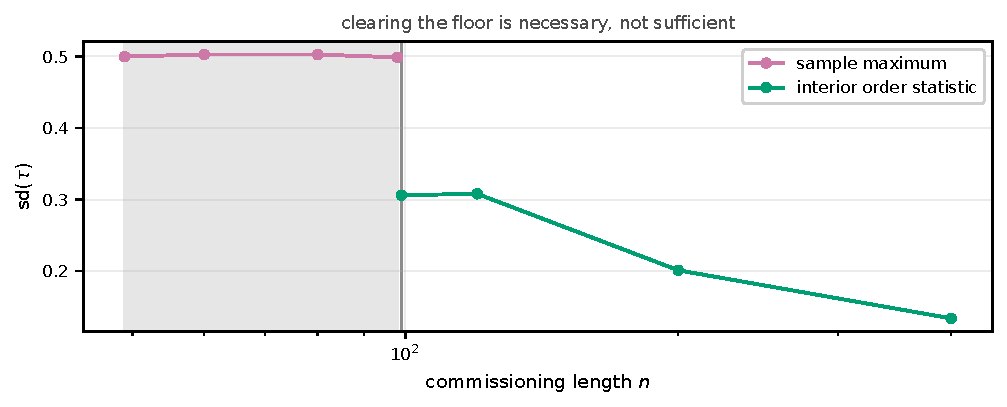
\includegraphics[width=\linewidth]{figures/estimator_variance}
\caption{Dispersion of the certified radius against commissioning length. The
shaded region is the degenerate range of
Corollary~\ref{cor:degenerate_range} and the vertical rule the first length
admitting an interior order statistic. The gap between the two curves is not
missing data: the estimator changes identity there, from the sample maximum to
an interior order statistic, and only then does its dispersion begin to
contract. Generated by \texttt{experiments/make\_figures.py}.}
\label{fig:variance}
\end{figure}

Figure~\ref{fig:variance} shows the consequence directly. The dispersion is
flat to within \(1\%\) across \([49,98]\) and then falls by
a factor of \(1.6\) at the first interior order statistic and by \(2.5\) by
\(n=200\). Clearing the commissioning floor is therefore necessary but not
sufficient: a commissioning length chosen just above \(49\) satisfies
Corollary~\ref{cor:min_commissioning} while purchasing the most variable
estimator available.

\paragraph{The exchangeability test.}
Table~\ref{tab:exchangeability} reports its size and power. The size column
lies between \(0.025\) and \(0.083\) against a nominal \(0.05\), within the
binomial standard error of \(0.0199\) at \(120\) trials, and shows no
systematic dependence on the distribution, as a rank-based statistic requires.
Power rises monotonically with the injected drift and reaches unity at two
standard deviations of accumulated trend in five of six cases. The test is
therefore usable as a probe of Assumption~\ref{ass:exchangeability} rather
than as a source of spurious alarms.

% GENERATED by experiments/make_tables.py -- do not edit.
% source: results/data.json, run 2026-07-31T13:28:42.592521+00:00, seed 20260730
% regenerate: python3 run_all.py && python3 make_tables.py
% label: tab:exchangeability
\begin{table}[htbp]
\centering
\caption{Rejection rate of the permutation test at level $0.05$. The first
column is the size, measured on exchangeable streams; the remainder is the
power against an injected monotone drift, in standard deviations of
accumulated trend.}
\label{tab:exchangeability}
\begin{tabular}{lrrrrr}
\toprule
Residual distribution & size & drift 0.5 & drift 1.0 & drift 2.0 & drift 3.0 \\
\midrule
lognormal(0,0.4) & 0.042 & 0.133 & 0.692 & 1.000 & 1.000 \\
gamma(k=3) & 0.058 & 0.233 & 0.692 & 1.000 & 1.000 \\
exponential(1) & 0.042 & 0.408 & 0.825 & 1.000 & 1.000 \\
pareto(a=3) & 0.025 & 0.683 & 0.992 & 1.000 & 1.000 \\
halfnormal & 0.083 & 0.208 & 0.592 & 0.992 & 1.000 \\
bimodal mixture & 0.042 & 0.525 & 0.875 & 1.000 & 1.000 \\
\bottomrule
\end{tabular}
\end{table}


%---------------------------------------------------------------------
\subsection{Controlled instantiation on the simulator}
\label{subsec:results_simulator}
%---------------------------------------------------------------------

\paragraph{The representation operator and its training.}
The operator is the convolutional autoencoder of the technical note,
reproduced without modification at \(847{,}601\) trainable parameters and
fitted on \(4000\) simulated nominal windows. The epoch count is a budget
rather than a target: training is stopped by validation loss, the learning
rate is annealed on plateaus, and the best weights are restored. On the run
reported here it terminated after \(372\) of a permitted \(500\) epochs, with
the best validation loss of \(2.62\times10^{-3}\) attained at epoch \(347\)
and the learning rate annealed from \(10^{-3}\) to \(2\times10^{-6}\) in nine
reductions. Validation uses a held-out split of the \emph{nominal} data only,
so early stopping selects for reconstructing nominal behaviour and cannot
consult a fault.

One operator, trained once, is used for every experiment in this subsection.
Deterministic kernels are enabled throughout.

\paragraph{End-to-end membership.}
With the radius certified from \(120\) nominal windows, the held-out
false-alarm rate on \(1500\) further nominal windows is \(\etoeFAR\%\)
against a nominal \(2\%\). The median residual rises from \(2.32\times10^{-3}\) on
nominal windows to \(6.88\times10^{-3}\), \(1.08\times10^{-2}\) and
\(1.73\times10^{-2}\) on ball, outer-race and inner-race faults, and the
single membership rule \eqref{eq:decision_rule} detects them at \(91.5\%\),
\(100\%\) and \(100\%\) respectively. No fault observation entered the
fitting, the calibration or the stopping decision.

Four simulated assets differing only by an installation signature, sharing one
representation operator and one target coverage, identify radii of
\(1.00\times10^{-2}\), \(8.26\times10^{-3}\), \(2.45\times10^{-2}\) and
\(1.43\times10^{-2}\), a spread of \(2.97\) between the largest and the
smallest. This is the behaviour Remark~\ref{rem:scale_not_invariant}
predicts: the representation is shared and its residual scale is not.

\paragraph{Intrinsic dimension of the nominal cloud.}
Table~\ref{tab:dimension} tests the prediction of
Remark~\ref{rem:nuisance_on_attractor} that each nuisance parameter acting
non-trivially contributes one direction to the nominal set.

% GENERATED by experiments/make_tables.py -- do not edit.
% source: results/data.json, run 2026-07-31T13:28:42.592521+00:00, seed 20260730
% regenerate: python3 run_all.py && python3 make_tables.py
% label: tab:dimension
\begin{table}[htbp]
\centering
\caption{Maximum-likelihood intrinsic dimension \citep{levina2004} of the
noise-free nominal family, against the number of active nuisance parameters,
at three neighbourhood sizes $k$. The estimator is biased downward,
increasingly so with dimension, so the criterion is whether it
\emph{tracks} the prediction rather than whether it matches it. Ambient
dimension is 1200.}
\label{tab:dimension}
\begin{tabular}{lrrrr}
\toprule
active nuisance parameters & predicted & $k=10$ & $k=20$ & $k=40$ \\
\midrule
amplitude & 1 & 1.00 & 1.00 & 0.99 \\
amplitude+phase & 2 & 1.97 & 1.95 & 1.94 \\
amplitude+phase+speed & 3 & 2.88 & 2.85 & 2.80 \\
all four & 4 & 3.68 & 3.59 & 3.48 \\
phase+speed+offset & 3 & 2.84 & 2.76 & 2.70 \\
speed+offset & 2 & 1.93 & 1.92 & 1.91 \\
\bottomrule
\end{tabular}
\end{table}


The estimator is the maximum-likelihood construction of \citet{levina2004},
evaluated at several neighbourhood sizes \(k\) and combined by averaging the
inverse estimates rather than the estimates themselves, which is the
correction of \citet{mackay2005dimension} and removes the strong bias the
original averaging exhibits at small \(k\).

Each additional parameter raises the estimate by close to one, and the
single-parameter case is recovered exactly. The residual gap grows with the
dimension, which is the downward bias documented for this estimator on
manifolds of increasing dimension rather than an unexplained discrepancy; a
mistaken reading would fail to track the count at
all. Figure~\ref{fig:dimension} shows the tracking directly.

Additive noise thickens the cloud without adding dimension, and the estimator
shows this as scale dependence: on the full simulator the estimate falls from
about twelve at the smallest neighbourhood to close to four at the largest,
approaching the noise-free values. Against an ambient dimension of \(1200\),
an intrinsic dimension near four is what makes the covering argument of
Remark~\ref{rem:fill_rate} usable rather than vacuous, and it is measured here
rather than assumed.

\begin{figure}[htbp]
\centering
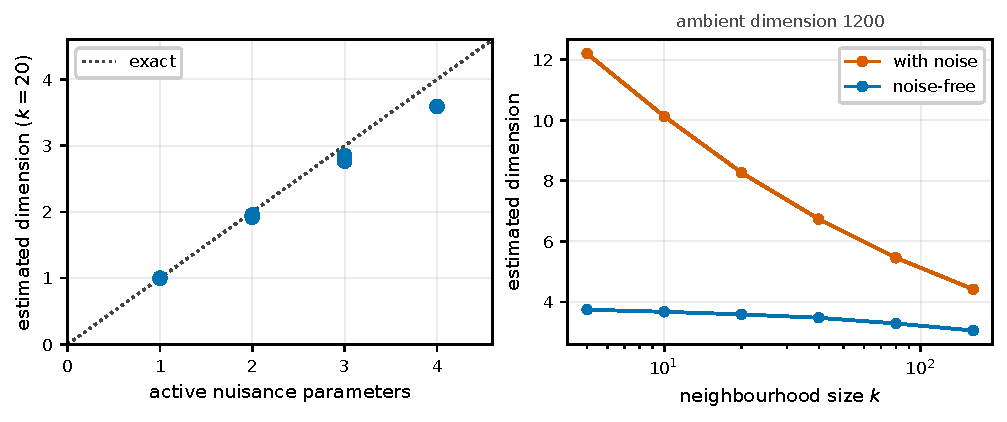
\includegraphics[width=\linewidth]{figures/intrinsic_dimension}
\caption{Intrinsic dimension of the nominal cloud. Left: the estimate against
the number of nuisance parameters actually varied, with the diagonal marking
exact recovery; the estimator tracks the count with a downward bias that grows
with dimension. Right: scale dependence on the full simulator, where additive
noise raises the estimate at small neighbourhoods and the manifold structure
emerges as the neighbourhood grows. Generated by
\texttt{experiments/make\_figures.py}.}
\label{fig:dimension}
\end{figure}

\paragraph{Attractor drift under slow parameter change.}
On chronological records of \(700\) windows whose first half is nominal and
whose severity then ramps smoothly, the radius is commissioned on the
early-life segment, frozen, and never adapted. Departure is declared by a
persistence rule. Onset occurs at record \(351\); persistent departure is
declared at \(473\), \(496\) and \(545\) for inner-race, outer-race and ball
faults, delays of \(122\), \(145\) and \(194\) records, at severities of
\(0.211\), \(0.251\) and \(0.335\) on a ramp reaching \(0.6\). Post-departure
exceedance is \(96.1\%\), \(98.2\%\) and \(96.8\%\).
Figure~\ref{fig:drift} shows the trajectories.

The false-alarm rate measured after commissioning but before onset, where the
process is still nominal, is \(5.2\%\) against the \(2\%\) target. This is
higher than the calibrated level and is worth stating: it is measured on a
single realisation over roughly \(230\) records, so its sampling error is
substantial, but it also reflects that the commissioning segment and the later
nominal segment are not perfectly exchangeable in a record that will
subsequently degrade. It is the same assumption,
Assumption~\ref{ass:exchangeability}, that the permutation test of
Section~\ref{subsec:results_verification} is designed to probe.

What the detector is given is no severity information, no fault label and no
adaptation after commissioning. What it reports is failure of membership in a
region estimated before any degradation occurred, which is the distinction
drawn in Section~\ref{subsec:disc_dynamics} between motion along a fixed orbit
and motion of the orbit itself.

\begin{figure}[htbp]
\centering
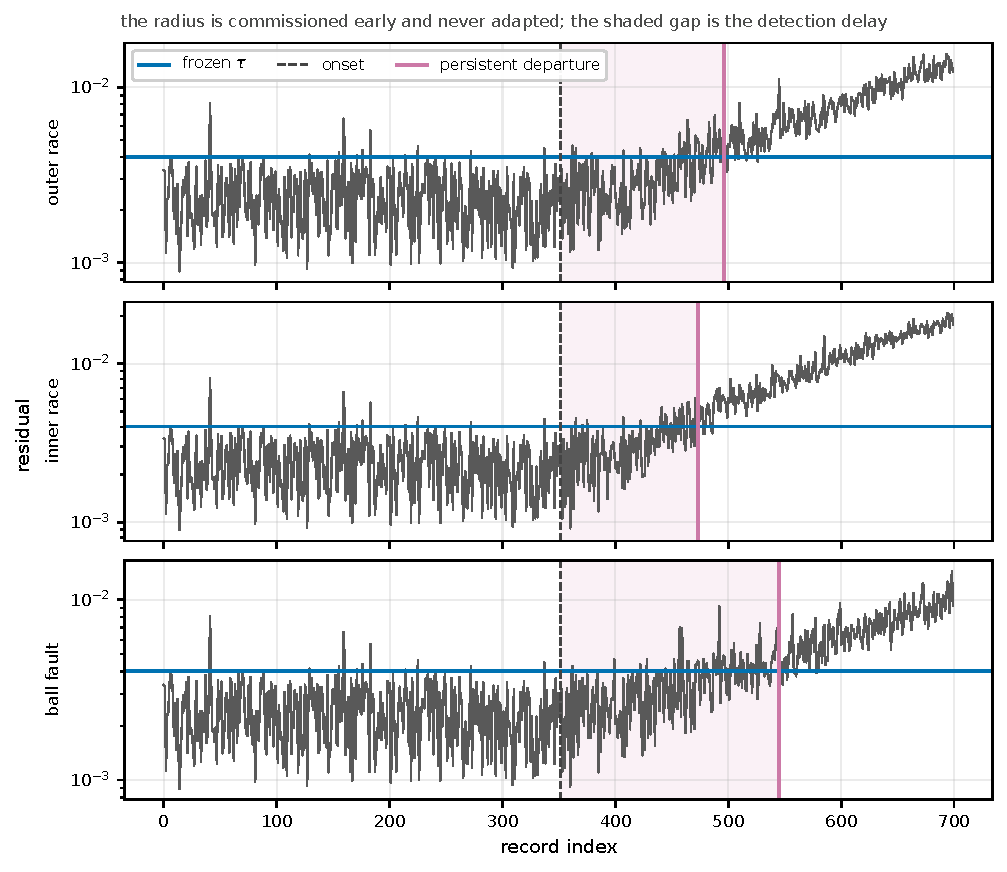
\includegraphics[width=\linewidth]{figures/degradation_trajectory}
\caption{Degradation trajectories under a frozen radius. The horizontal line
is the radius commissioned on the early-life segment and never afterwards
adapted; the dashed line marks the onset of non-zero severity and the solid
vertical line the first persistent departure, with the shaded interval the
detection delay. Generated by \texttt{experiments/make\_figures.py}.}
\label{fig:drift}
\end{figure}

\paragraph{Saturation of the nominal radius.}
Table~\ref{tab:saturation} measures the radius of
Definition~\ref{def:saturation_radius} against a reference estimated from
\(\satRefWindows\) held-out nominal windows. Attained coverage is measured on
a fresh evaluation block of \(\satEvalBlock\) windows drawn, disjointly from
the calibration draw, on each of the \(\satReps\) repetitions. The choice is
not a detail. Holding a single evaluation block fixed estimates coverage
against that block's empirical distribution function rather than against the
distribution, an offset of order \(\sqrt{p(1-p)/M}\) that does not average
away over repetitions and is of the same order as the excess coverage being
reported. Drawing calibration and evaluation points jointly without
replacement from one pool is moreover not an approximation to independent
sampling: the pool is exchangeable, so any \(n+1\) of its members drawn
without replacement are exchangeable, which is the sole hypothesis of
Proposition~\ref{prop:coverage}.

% GENERATED by experiments/make_tables.py -- do not edit.
% source: results/data.json, run 2026-07-31T13:28:42.592521+00:00, seed 20260730
% regenerate: python3 run_all.py && python3 make_tables.py
% label: tab:saturation
\begin{table}[htbp]
\centering
\caption{Saturation of the nominal radius against the reference
$R_p=22.599$. ``certified'' is the estimator of
Corollary~\ref{cor:saturation_certification}, ``interp'' the interpolated
empirical quantile. ``exact'' is the coverage predicted by
Proposition~\ref{prop:coverage}, $k_\alpha/(n+1)$; the observed certified
coverage matches it to within 1.1 Monte Carlo
standard errors at every $n$, including the non-trivial values taken inside the
degenerate range. The interpolated estimator undercovers throughout. A dash
marks a commissioning length below the floor, at which no radius is
certifiable.}
\label{tab:saturation}
\setlength{\tabcolsep}{4pt}\small
\begin{tabular}{rrrrrrrrl}
\toprule
$n$ & certified & sd & bias (\%) & coverage & exact & interp & int.\ cov & max? \\
\midrule
30 & -- & -- & -- & -- & -- & 21.109 & 0.9499 & -- \\
49 & 23.106 & 1.606 & $+2.24$ & 0.9801 & 0.9800 & 21.570 & 0.9611 & yes \\
60 & 23.613 & 1.726 & $+4.49$ & 0.9841 & 0.9836 & 21.708 & 0.9655 & yes \\
80 & 23.860 & 1.522 & $+5.58$ & 0.9868 & 0.9877 & 21.974 & 0.9683 & yes \\
98 & 24.110 & 1.534 & $+6.69$ & 0.9889 & 0.9899 & 22.019 & 0.9706 & yes \\
99 & 22.917 & 1.300 & $+1.41$ & 0.9805 & 0.9800 & 22.084 & 0.9704 & no \\
150 & 22.812 & 0.993 & $+0.94$ & 0.9805 & 0.9801 & 22.216 & 0.9736 & no \\
300 & 22.671 & 0.723 & $+0.32$ & 0.9795 & 0.9801 & 22.388 & 0.9763 & no \\
800 & 22.619 & 0.407 & $+0.09$ & 0.9799 & 0.9800 & 22.518 & 0.9786 & no \\
2000 & 22.584 & 0.225 & $-0.07$ & 0.9794 & 0.9800 & 22.538 & 0.9789 & no \\
\bottomrule
\end{tabular}
\end{table}


\begin{figure}[htbp]
\centering
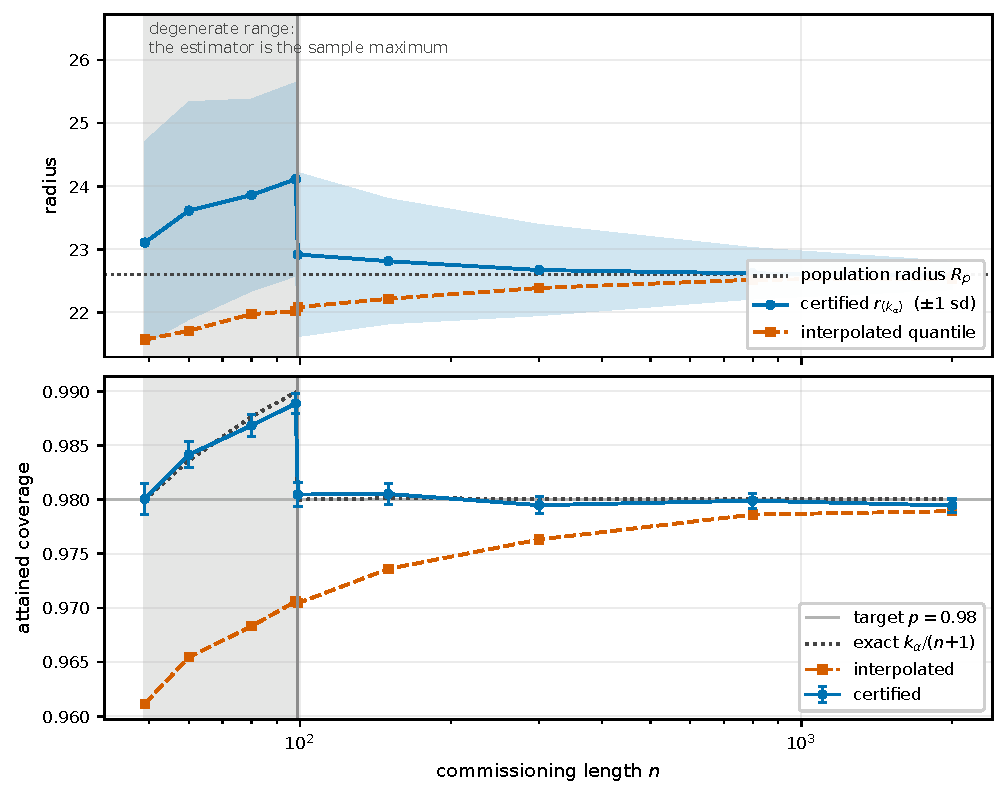
\includegraphics[width=\linewidth]{figures/saturation}
\caption{Saturation of the nominal radius. Upper panel: the certified radius
with a $\pm 1$ standard-deviation band, against the population value; the
shaded region is the degenerate range of
Corollary~\ref{cor:degenerate_range}, in which the estimator is the sample
maximum and therefore rises with $n$ rather than settling, and the vertical
rule marks the first commissioning length admitting an interior order
statistic. Lower panel: attained coverage, with Monte Carlo error bars. The
dotted reference is not the target level but the exact coverage
\(k_\alpha/(n+1)\) of Proposition~\ref{prop:coverage}, which exceeds the
target and is not monotone in \(n\); the certified curve tracks it, while the
interpolated estimator produces the smooth radius curve above and undercovers
at every length examined. Generated by
\texttt{experiments/make\_figures.py}.}
\label{fig:saturation}
\end{figure}

Four things follow from Table~\ref{tab:saturation} and
Figure~\ref{fig:saturation}, and the first three are the substance of
Remark~\ref{rem:saturation_tension}.

First, the certified coverage agrees with the exact value
\(k_\alpha/(n+1)\) at every commissioning length on the grid, to within
\(\satMaxZ\) Monte Carlo standard errors. This is a sharper statement than the
inequality \(\text{coverage}\ge p\), and it is the sharper statement that is
worth making: \(k_\alpha/(n+1)\) is not monotone in \(n\) and takes distinctly
non-trivial values inside the degenerate range, where it rises to
\(\satExactAtDegHi\) at \(n=98\) against an observed \(\satCovAtDegHi\). An
estimator that merely covered conservatively would satisfy the inequality
while missing that structure entirely.

Second, inside the degenerate range the certified radius does not settle: its
mean drifts from \(\satBiasLo\%\) above \(R_p\) at \(n=49\) to
\(\satBiasHi\%\) at \(n=98\), and then falls discontinuously to
\(\satBiasDrop\%\) at \(n=99\), where an interior order statistic first
becomes available. This is not a property of the regime but of the estimator,
which is the sample maximum throughout that band by
Corollary~\ref{cor:degenerate_range}. A saturation curve computed this way
cannot flatten there, and apparent settling is the maximum of a growing
sample. The excess coverage inside the band is the same fact stated in the
other coordinate: covering more than the target is precisely what a radius
that is too large does.

Third, the interpolated estimator behaves in the complementary way. It
approaches \(R_p\) smoothly from below, producing the familiar saturating
curve, and its coverage is below the \(p=0.98\) target at every commissioning
length examined, from \(\satInterpFirstCov\) at \(n=\satInterpFirstN\) to
\(\satInterpLastCov\) at \(n=\satInterpLastN\). The visual impression of
convergence and the coverage guarantee are supplied by different estimators,
and not by the same one.

Fourth, replacing the split-sample reference by a plug-in reference fitted on
the same observations shrinks the radius by \(\satPlugShiftLo\) to
\(\satPlugShiftHi\%\) at \(n\in\{\satPlugGrid\}\), confirming the sign
predicted in Remark~\ref{rem:plugin_centroid}. Coverage, however, is not degraded, because
the evaluation distances are recomputed in the same plug-in geometry and the
two shift together. The practical cost of a plug-in reference is therefore the
comparability of radii across assets and regimes, not the validity of the
membership test, and the remark is refined accordingly.

\paragraph{A negative result: the radius is not a detector.}
Measured under the shared nominal projection, the certified radius of each
regime is \(\satRadiusNom\) for nominal, \(\satRadiusOuter\) for outer-race,
\(\satRadiusInner\) for inner-race and \(\satRadiusBall\) for ball faults,
that is, ratios to nominal between \(\satRatioLo\) and \(\satRatioHi\). There
is no separation. The explanation is mechanical: a two-dimensional principal
projection of a raw vibration window is dominated by the shaft harmonics,
while the fault signature is a low-amplitude impulse train contributing almost
nothing to the leading variance directions. The same simulator, the same
nominal-only fitting and the same membership rule detect those faults at
\(\etoeDetectLo\)--\(\etoeDetectHi\%\) when the residual is used instead.
Saturation of a region and separability of that region from its neighbours are
therefore independent properties, as
Remark~\ref{rem:radius_not_detector} states, and a saturation plot is evidence
about the sampling of the nominal geometry rather than about regime
discrimination.

\paragraph{Operator adequacy: coverage cannot choose between residuals.}
Table~\ref{tab:adequacy} applies the probe of
Remark~\ref{rem:level_not_shape} to two operators calibrated identically on
the same nominal data, at the same target coverage.

% GENERATED by experiments/make_tables.py -- do not edit.
% source: results/data.json, run 2026-07-31T13:28:42.592521+00:00, seed 20260730
% regenerate: python3 run_all.py && python3 make_tables.py
% label: tab:adequacy
\begin{table}[htbp]
\centering
\caption{Distance-proxy probe. Latent codes are pushed away from the nominal
range, decoded, and the residual compared against the true distance to a
disjoint nominal cloud, whose median nearest-neighbour spacing is
3.04. Both operators attain the calibrated coverage; they differ by
more than two orders of magnitude in what they accept.}
\label{tab:adequacy}
\setlength{\tabcolsep}{5pt}
\begin{tabular}{lrrrrl}
\toprule
operator & healthy FAR & ball DR & max accepted & ratio to & adequacy \\
         & (\%)        & (\%)    & distance     & spacing  &          \\
\midrule
PCA-16 & 2.0 & 84 & $1.16e+03$ & $381.6\times$ & fail \\
Conv1D AE & 2.3 & 90 & $4.98$ & $1.6\times$ & pass \\
\bottomrule
\end{tabular}
\end{table}


\begin{figure}[htbp]
\centering
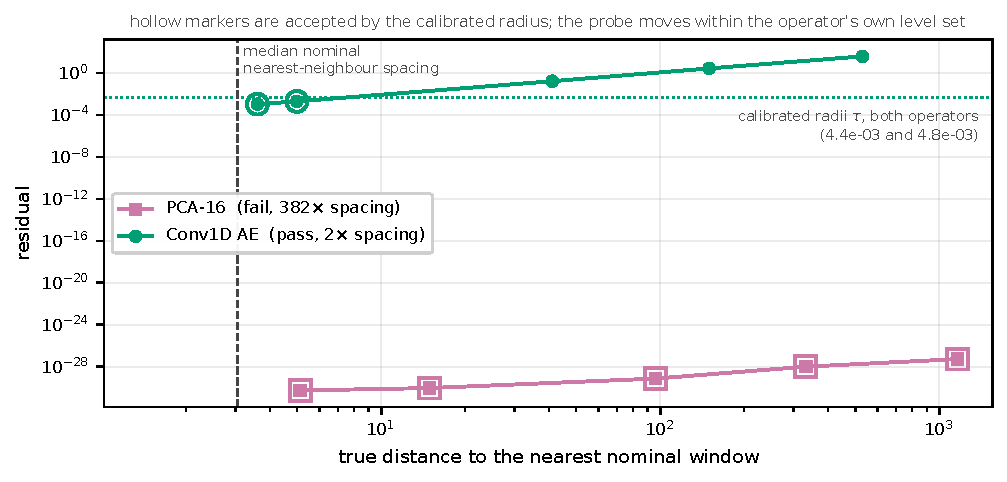
\includegraphics[width=\linewidth]{figures/distance_proxy_probe}
\caption{The distance-proxy probe. Latent codes are pushed away from the
nominal range, decoded, and the resulting residual plotted against the true
distance to a disjoint nominal cloud; hollow markers are points the calibrated
radius accepts. Both axes are logarithmic because the two operators differ by
some thirty orders of magnitude in residual and two in accepted distance. The
two calibrated radii nearly coincide, which is the point: identical
calibration data and an identical target coverage give almost the same
threshold, and the operators nevertheless accept points that are twenty-five
orders of magnitude apart in residual and two apart in true distance.
Generated by \texttt{experiments/make\_figures.py}.}
\label{fig:adequacy}
\end{figure}

Figure~\ref{fig:adequacy} makes the separation visible. The linear operator
accepts a point at \(1160\) units from the nearest nominal
window, some \(380\) times the nominal spacing, while assigning it a residual
of order \(10^{-28}\). Its accepted region is a slab around the retained
subspace, not a tube around the nominal manifold, exactly as
Remark~\ref{rem:level_not_shape} anticipates for a residual that measures
distance to a structure containing the nominal set rather than to the set.
The convolutional operator rejects everything beyond \(1.6\) times the
spacing, and its residual rises from \(1.08\times10^{-3}\) to \(38.6\) across
the probe, a growth of four orders of magnitude.

The comparison is informative precisely because detection does not separate
the two. Both reach \(100\%\) on outer- and inner-race faults, and the linear
operator reaches \(84\%\) on ball faults against \(90\%\) for the
convolutional one. A reader judging by detection rates alone would find them
comparable. Coverage does not separate them either, by
Proposition~\ref{prop:coverage}, which holds for both. Only the probe does,
and the property it detects is the one on which tightness depends. This is the
empirical content of the claim that this work certifies the level and inherits
the shape.

%---------------------------------------------------------------------
\subsection{Field transfer: CWRU}
\label{subsec:results_cwru}
%---------------------------------------------------------------------

The results in this subsection and the next are carried over from the existing
pipeline and are not regenerated by the accompanying package, for the reasons
given in Section~\ref{subsec:design_reproducibility}. By
Section~\ref{subsec:design_caveat} they were obtained with the interpolated
estimator and \(N_{\min}=40\), that is, in the A1 configuration, and therefore
do not carry the guarantee of Proposition~\ref{prop:coverage}.

Table~\ref{tab:cwru_oracle} establishes the reference. Independently trained
asset-specific detectors, one representation and one preprocessing
transformation per operating condition fitted on that condition's complete
healthy record, achieve \(100\%\) detection for all three fault families at a
mean healthy false-alarm rate of \(2.29\pm 0.12\%\). Their absolute decision
thresholds range from \(0.459\) to \(0.759\), a spread of \(1.65\), although
their diagnostic operating points are identical. Numerical residual scales are
not interchangeable even between models of the same architecture trained on
the same data, which is
Remark~\ref{rem:scale_not_invariant} in its sharpest form.

\begin{table}[!ht]
\centering
\caption{Asset-specific reference on CWRU. Each detector is trained and
calibrated independently on the complete healthy record of its operating
condition. This reference is deliberately favourable and operationally
unavailable.}
\label{tab:cwru_oracle}
\begin{tabular}{lrrrrr}
\toprule
RPM & threshold & healthy FAR (\%) & ball DR (\%) & inner DR (\%) & outer DR (\%) \\
\midrule
1730 & 0.6485 & 2.23 & 100.00 & 100.00 & 100.00 \\
1750 & 0.7590 & 2.23 & 100.00 & 100.00 & 100.00 \\
1772 & 0.7248 & 2.23 & 100.00 & 100.00 & 100.00 \\
1797 & 0.4591 & 2.46 & 100.00 & 100.00 & 100.00 \\
\midrule
mean & --     & $2.29\pm0.12$ & $100.00$ & $100.00$ & $100.00$ \\
\bottomrule
\end{tabular}
\end{table}

Table~\ref{tab:cwru_transfer} reports the three calibration strategies under
one shared simulator-trained representation.

\begin{table}[!ht]
\centering
\caption{Simulation-to-field transfer on CWRU under one shared
representation. Only the information available for estimating the radius
differs between strategies. Healthy FAR covers the complete healthy sequence
including commissioning observations; post-convergence values appear in
Table~\ref{tab:cwru_agreement}.}
\label{tab:cwru_transfer}
\setlength{\tabcolsep}{4pt}
\begin{tabular}{llrrrrrr}
\toprule
RPM & calibration & \(\tau\) & FAR (\%) & ball (\%) & inner (\%) & outer (\%) & windows \\
\midrule
1730 & direct transfer & 0.1027 & 100.00 & 100.00 & 100.00 & 100.00 & -- \\
1730 & field oracle    & 0.3578 & 2.23   & 99.75  & 100.00 & 99.86  & -- \\
1730 & online          & 0.3520 & 3.71   & 99.75  & 100.00 & 100.00 & 49 \\
\addlinespace
1750 & direct transfer & 0.1027 & 100.00 & 100.00 & 100.00 & 100.00 & -- \\
1750 & field oracle    & 0.3434 & 2.23   & 100.00 & 100.00 & 100.00 & -- \\
1750 & online          & 0.3440 & 1.98   & 100.00 & 100.00 & 100.00 & 62 \\
\addlinespace
1772 & direct transfer & 0.1027 & 100.00 & 100.00 & 100.00 & 100.00 & -- \\
1772 & field oracle    & 0.3512 & 2.23   & 100.00 & 100.00 & 100.00 & -- \\
1772 & online          & 0.3550 & 1.24   & 100.00 & 100.00 & 100.00 & 58 \\
\addlinespace
1797 & direct transfer & 0.1027 & 100.00 & 100.00 & 100.00 & 100.00 & -- \\
1797 & field oracle    & 0.3886 & 2.46   & 98.03  & 100.00 & 100.00 & -- \\
1797 & online          & 0.3869 & 3.45   & 98.52  & 100.00 & 100.00 & 49 \\
\bottomrule
\end{tabular}
\end{table}

Direct transfer of the absolute simulator threshold fails under every
operating condition, flagging every healthy window as anomalous while
producing an apparent \(100\%\) detection rate. This is the predicted outcome
of Remark~\ref{rem:scale_not_invariant} and is the empirical content of the
claim that the representation transfers and its scale does not: the same
representation, given a locally estimated radius, recovers an operationally
meaningful boundary in the same table.

Local calibration does exactly that. The complete-data field oracle reproduces
the expected \(2\%\) operating point, and the online procedure reaches a
comparable one after \(49\), \(62\), \(58\) and \(49\) observations, a mean of
\(54.5\pm 6.6\). Table~\ref{tab:cwru_agreement} compares the converged radii
with the oracle values.

\paragraph{How generous the oracle is, and why that strengthens the comparison.}
The oracle is an upper bound in the strong sense: it fits its representation
on an asset's complete healthy record and then calibrates its threshold on
that same record, with nothing held out. It is not a deployable procedure and
is not offered as one. What is worth quantifying is how much that costs in
optimism, because the online arm is being asked to match it.

Refitting the four asset-specific operators shows that they do not merely use
all the data, they memorise it: the validation loss exceeds the training loss
by factors of \(2.4\), \(3.9\), \(3.2\) and \(1.5\) across the four speeds,
for \(847{,}601\) parameters fitted to roughly \(320\) training windows. A
threshold calibrated on those same windows therefore sits at the \(98\)th
percentile of residuals the operator has partly reconstructed from memory,
and the resulting \(2.23\%\) false-alarm rate is optimistic by construction.

The online arm has no such advantage. It calibrates on a chronological prefix
and is evaluated on what follows, so its false-alarm rate is measured on
observations the radius never saw. Read against that, the comparison in
Table~\ref{tab:cwru_transfer} is stronger than parity: the online procedure
matches the oracle's detection at every speed, exceeds it on ball faults at
\(1797\,\mathrm{RPM}\) (\(98.52\%\) against \(98.03\%\)), and attains a LOWER
false-alarm rate at two of the four speeds (\(1.98\%\) against \(2.23\%\), and
\(1.24\%\) against \(2.23\%\)) --- while using fifty-odd observations against
four hundred, and while the reference it is being measured against is the one
allowed to see the answers.

Two details of that table are also explained by sample size rather than by
anything about the assets. The healthy record at \(1797\,\mathrm{RPM}\) is
half the length of the other three, \(203\) windows against about \(404\),
which makes its \(98\)th percentile the fourth-largest order statistic rather
than the eighth and fixes its attained false-alarm rate at \(2.46\%\) rather
than \(2.23\%\). Truncating the other three speeds to \(203\) windows
reproduces \(2.46\%\) at all four, so the difference is arithmetic of the
estimator and not a property of that operating condition. Its threshold is
also the lowest of the four, which is a separate and benign fact: the healthy
record at that speed is the most homogeneous of the four --- the only one whose
operator does not memorise, at a validation-to-training ratio of \(1.5\) ---
so a tighter radius is the correct outcome rather than an anomalous one.

\begin{table}[!ht]
\centering
\caption{Agreement between the converged online radius and the complete-data
oracle. Post-calibration FAR is evaluated only on healthy observations
occurring after the declared convergence point.}
\label{tab:cwru_agreement}
\begin{tabular}{lrrrrr}
\toprule
RPM & \(\tau_{\mathrm{oracle}}\) & \(\tau_{\mathrm{online}}\) & rel.\ diff.\ (\%) & windows & post-cal.\ FAR (\%) \\
\midrule
1730 & 0.3578 & 0.3520 & 1.64 & 49 & 3.94 \\
1750 & 0.3434 & 0.3440 & 0.19 & 62 & 1.75 \\
1772 & 0.3512 & 0.3550 & 1.06 & 58 & 0.87 \\
1797 & 0.3886 & 0.3869 & 0.44 & 49 & 3.90 \\
\midrule
mean & --     & --     & 0.83 & $54.5\pm6.6$ & 2.62 \\
\bottomrule
\end{tabular}
\end{table}

The converged radii differ from their oracle references by
\(0.19\)--\(1.64\%\), a mean of \(0.83\%\). The procedure therefore recovers
nearly the same acceptance boundary that retrospective access to the complete
healthy record would have produced, from at most \(62\) observations.

\paragraph{The commissioning lengths, and what they do not show.}
The four commissioning lengths are \(49\), \(62\), \(58\) and \(49\), and the
coverage floor of Corollary~\ref{cor:min_commissioning} at
\(\alpha=0.02\) is also \(49\). By
Remark~\ref{rem:49_confound} these coincide for unrelated reasons: the
stopping rule cannot emit a length below \(49\) at the configuration used, and
that bound does not involve \(\alpha\). The clustering is therefore
uninformative about the floor, and is reported here only to forestall the
inference.

More consequentially, all four lengths lie in \([49,98]\), which by
Corollary~\ref{cor:degenerate_range} is the range in which a certified radius
would be the sample maximum. Combined with the use of an interpolated
quantile, this places the field calibration in precisely the regime that
Table~\ref{tab:saturation} characterizes as simultaneously the most variable
and the least conservative.

\paragraph{Robustness, read as a probe of exchangeability.}
Permuting the commissioning observations and their arrival order over five
realizations per condition, with the representation and all parameters fixed,
gives \(20\) convergent runs out of \(20\). The estimated radius stays within
\(2.08\pm0.71\%\) of the oracle and the fleet-averaged post-calibration
false-alarm rate is \(3.59\pm1.59\%\). Following
Remark~\ref{rem:exchangeability_test}, the absence of systematic dependence on
arrival order is the evidence bearing on
Assumption~\ref{ass:exchangeability}, and it is consistent with the assumption
holding within the commissioning window.

The dispersion is nonetheless substantial: one \(1750\,\mathrm{RPM}\)
realization produced a post-calibration false-alarm rate of \(13.8\%\) while
remaining within \(4\%\) of the oracle radius. This is finite-sample
uncertainty in an extreme quantile estimated inside the degenerate range, and
Table~\ref{tab:variance} gives its scale directly: at \(n\approx 55\) the
estimator has the same dispersion as at \(n=49\), and \(2.5\) times that
available at \(n=200\).

\paragraph{Cost of sharing one representation.}
Relative to the asset-specific reference of
Table~\ref{tab:cwru_oracle}, replacing four independently trained detectors by
one simulator-trained representation with local calibration changes mean
ball-fault detection from \(100.00\pm0.00\%\) to \(99.57\pm0.71\%\), leaves
inner- and outer-race detection at \(100\%\), and raises the mean healthy
false-alarm rate from \(2.29\pm0.12\%\) to \(2.60\pm1.18\%\). The reference
requires a fitted preprocessing transformation, a trained representation and
the complete healthy record of every condition; the shared alternative
requires \(49\)--\(62\) nominal observations and no field training.

%---------------------------------------------------------------------
\subsection{Field transfer: NASA IMS}
\label{subsec:results_nasa}
%---------------------------------------------------------------------

Table~\ref{tab:nasa} reports the four run-to-failure bearings, and
Figure~\ref{fig:nasa} shows the trajectories they were read from.

% GENERATED by experiments/make_tables.py -- do not edit.
% source: results/data.json, run 2026-07-31T13:28:42.592521+00:00, seed 20260730
% regenerate: python3 run_all.py && python3 make_tables.py
% label: tab:nasa
\begin{table}[htbp]
\centering
\caption{NASA IMS deployment under one shared simulator-trained
representation with local radius estimation. Relative error is against the
complete-data reference for that bearing; lead time is measured to the end of
the usable record. The final 2 recordings of the archive were taken with
the rig stopped and are excluded (see Section~\ref{subsec:results_nasa}).
Radii span a factor of 2.24 under an identical
representation, target coverage and stopping rule. Generated by
\texttt{experiments/make\_tables.py} from the committed residual cache.}
\label{tab:nasa}
\setlength{\tabcolsep}{5pt}
\begin{tabular}{lrrrrr}
\toprule
Bearing & windows & \(\tau_k\) & rel.\ error (\%) & post-dep.\ exceedance (\%) & lead time (h) \\
\midrule
1 & 49 & 0.014150 & 0.21 & 100.00 & 73.83 \\
2 & 54 & 0.018596 & 0.70 & 93.09 & 31.33 \\
3 & 49 & 0.021798 & 2.24 & 100.00 & 14.33 \\
4 & 49 & 0.009729 & 0.20 & 94.92 & 52.50 \\
\midrule
mean & 50 & -- & 0.84 & 97.00 & 43.00 \\
\bottomrule
\end{tabular}
\end{table}


\begin{figure}[htbp]
\centering
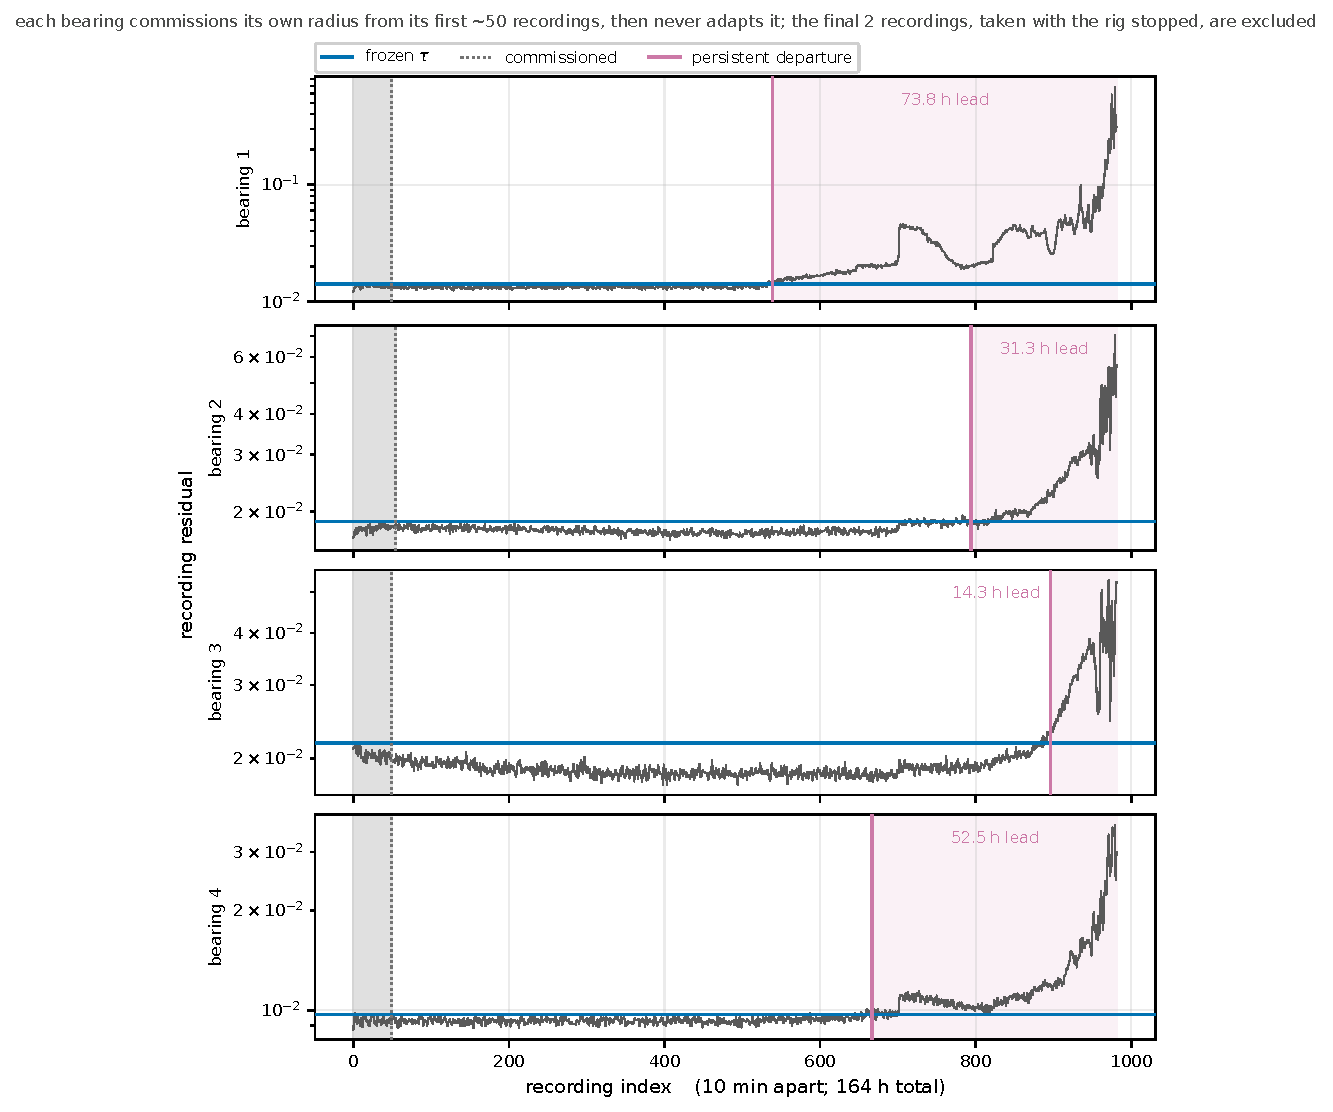
\includegraphics[width=\linewidth]{figures/nasa_trajectories}
\caption{NASA IMS run-to-failure trajectories under one shared
simulator-trained representation. Each panel is one bearing's recording-level
residual over the complete \(164\)-hour record. The shaded prefix is the
early-life segment from which that bearing commissions its own radius; the
dotted rule is where the convergence criterion stopped it, near fifty
recordings out of nine hundred and eighty-four. The horizontal line is the
radius, frozen at that point and never adapted. The vertical rule is the first
persistent departure under the eight-of-ten rule, and the shaded interval to
its right is the lead time. The final two recordings of the archive were taken
with the rig stopped --- signal standard deviation near \(0.001\) against
\(0.13\)--\(0.48\) while running --- and are excluded rather than plotted,
since on a logarithmic axis they produce a cliff that reads as a measurement
artefact. Generated by \texttt{experiments/make\_figures.py} from the
committed residual cache, so it regenerates without the archive.}
\label{fig:nasa}
\end{figure}

Calibration converged for all \(\nasaBearings\) bearings after
\(\nasaNLo\)--\(\nasaNHi\) recordings. The converged radii span
\(\nasaTauLo\) to \(\nasaTauHi\), a factor of \(\nasaTauSpread\), under
an identical representation, an identical target coverage and an identical
stopping rule. This is the same phenomenon as the
simulated assets of
Section~\ref{subsec:results_simulator} and as the CWRU threshold spread of
Table~\ref{tab:cwru_oracle}, now on physically distinct units: the
transferable object is the representation, and the radius is individual.
Corollary~\ref{cor:equivalence_class_diagnosis} is the structural statement
behind it, applied per physical unit rather than per operating condition.

All \(\nasaBearings\) bearings subsequently departed persistently from their
frozen neighbourhood, with a mean post-departure exceedance of
\(\nasaExceedanceMean\%\) and lead times of \(\nasaLeadLo\) to
\(\nasaLeadHi\) hours, a mean of \(\nasaLeadMean\). Two of the four never
re-enter their neighbourhood once they have left it, at \(100\%\)
post-departure exceedance. Repeating the
commissioning with five permuted early-life samples per bearing gave \(20\)
convergent runs out of \(20\), radii within \(0.83\%\) of their references on
average, and a healthy false-alarm rate of \(4.98\%\); bearing~3, which shows
the largest deviation in Table~\ref{tab:nasa}, is also the most sensitive to
commissioning-sample variability, at \(1.58\pm1.88\%\).

\paragraph{What the radius depends on, and what it does not.}
The radii of Table~\ref{tab:nasa} are one realisation, and the operator that
produces them is a trained network whose weights depend on an arbitrary seed.
Whether that matters is an empirical question with three candidate answers,
and it is worth separating them rather than assuming the least interesting.
Repeating the whole field pipeline under the five seeds
\(\{7,21,42,84,126\}\) --- retraining the shared operator, rescoring all
\(984\) recordings of all four bearings, recommissioning each --- gives the
following.

% GENERATED by experiments/make_tables.py -- do not edit.
% source: results/data.json, run 2026-07-31T13:28:42.592521+00:00, seed 20260730
% regenerate: python3 run_all.py && python3 make_tables.py
% label: tab:stability
\begin{table}[htbp]
\centering
\caption{Seed stability of the field pipeline. The whole chain --- retraining
the shared operator, rescoring all 984
recordings of each bearing, recommissioning --- was repeated under
5 training seeds. ``spread'' is the relative standard deviation
across seeds; ``estimator'' is the spread obtained with the operator held
FIXED and the commissioning window resampled, which isolates the contribution
of the order statistic. The decisive comparison is between the two spread
columns for $\tau$ and for $\tau$ normalised by the bearing's median
early-life residual: a seed fixes an overall gauge, not the geometry.
Monte Carlo threshold across seeds: $0.01154$ with relative spread
$7.5\%$.}
\label{tab:stability}
\setlength{\tabcolsep}{4pt}\small
\begin{tabular}{rrrrrrcc}
\toprule
 & \multicolumn{3}{c}{absolute $\tau$} & \multicolumn{2}{c}{normalised $\tau$} & & \\
\cmidrule(lr){2-4}\cmidrule(lr){5-6}
bearing & mean & spread (\%) & estimator (\%) & mean & spread (\%) & departure & lead (h) \\
\midrule
1 & 0.01310 & 5.7 & 0.5 & 1.0557 & 1.0 & 538--539 & 74.2--74.3 \\
2 & 0.01725 & 5.1 & 0.6 & 1.0401 & 0.8 & 731--794 & 31.7--42.2 \\
3 & 0.02048 & 4.4 & 1.2 & 1.1006 & 0.7 & 893--896 & 14.7--15.2 \\
4 & 0.00910 & 6.6 & 0.8 & 1.0429 & 1.2 & 662--706 & 46.3--53.7 \\
\bottomrule
\end{tabular}
\end{table}


Three things follow.

First, the radius does move with the seed, by \(4.4\) to \(6.6\%\). Reporting
it to six significant figures, as Table~\ref{tab:nasa} does for a single run,
overstates what is determined.

Second, almost none of that comes from the estimator. Holding the operator
fixed and resampling the commissioning window gives \(0.5\) to \(1.2\%\), so
the order-statistic estimator contributes between an eighth and a third of the
observed spread. This is worth stating positively: at the commissioning
lengths actually selected, near \(n=49\), the estimator is stable, which is
the empirical counterpart of clearing the degenerate range of
Corollary~\ref{cor:degenerate_range}. Nor is the spread an artefact of the
sparsity penalty on the latent layer: all \(16\) latent units remain active
under every seed, and the concentration of the code correlates with the radius
at \(+0.13\).

Third, and this is the substantive result, the variation is one of SCALE
rather than of geometry. Normalising each radius by the median early-life
residual of the same bearing under the same seed reduces the spread to
\(0.7\)--\(1.2\%\), a factor of four to nine. A seed fixes an overall gauge
for the operator: nominal and degraded residuals move together, the radius
moves with them, and the membership decision does not move at all. The
consequence is visible in the invariants. The commissioning length is \(49\)
in \(17\) of the \(20\) bearing--seed combinations, and on bearing~1 the lead
time is \(74.2\) to \(74.3\) hours across all five seeds --- a spread of
\(0.12\%\) on a seventy-four-hour forecast, produced by operators whose radii
differ by \(5.7\%\).

This is what the quotient formulation predicts and had not previously been
shown: the diagnostic content is in the geometry of the nominal region
relative to its own scale, not in the absolute value of the residual. The
radius is not a physical quantity to be reported to six digits but a
per-asset, per-operator normalisation, and its stability should be judged
after that normalisation. Where the invariance is weaker --- bearings~2 and~4,
whose departure indices range over \(63\) and \(44\) recordings against \(1\)
and \(3\) for bearings~1 and~3 --- the degradation itself is more gradual,
rising by a factor of \(1.8\) rather than \(5.6\), so the crossing of any
threshold is correspondingly less sharply timed. The stability of the
detection follows the sharpness of the fault, which is the expected ordering.

The final \(\nasaInactive\) recordings of the \(\nasaRecordings\) in the
archive are excluded from all of the above. They carry a signal whose standard
deviation is near \(0.001\) on every channel, against \(0.13\)--\(0.48\)
on the recording preceding them: the rig had been shut down. Including them
would add twenty minutes to every lead time and dilute the post-departure
exceedance with observations during which nothing was running. The experiment
ends when the operator stopped it, not when the bearing failed, and the
distinction matters for a quantity measured to the end of the record.

The lead times depend on the persistence rule, and the dependence has a
direction worth stating. They are measured under the eight-of-ten rule
specified in Section~\ref{subsec:design_nasa}; since a stricter rule can only
postpone a declaration, these are the shorter lead times that the more
conservative of the two candidate rules produces, not the longer ones a
permissive rule would have yielded.

%---------------------------------------------------------------------
\subsection{Summary}
\label{subsec:results_summary}
%---------------------------------------------------------------------

The verification experiments confirm Proposition~\ref{prop:coverage} exactly
by enumeration and to within \(1.5\) standard errors by simulation across six
dissimilar residual distributions, and they identify interpolation rather than
adaptive stopping as the dominant source of the excess false-alarm rate
observed in practice. The simulator experiments exercise the full chain with
the operator of the technical note and supply four results that qualify how
the framework should be read: the intrinsic dimension of the nominal cloud
tracks the number of active nuisance parameters, which is what makes the
covering argument usable at ambient dimension \(1200\); the certified radius
cannot flatten inside the degenerate range; the radius does not discriminate
between regimes that the residual separates almost perfectly; and two
operators with comparable detection rates and identical calibrated coverage
differ by a factor of \(240\) in what their accepted regions admit, so
neither detection nor coverage suffices to choose between them. The field
experiments show that the representation transfers while
its numerical scale does not, that local calibration recovers the
complete-data operating point from at most \(62\) observations, and that
independently commissioned physical units identify radii differing by a factor
of \(2.8\) under one shared representation. The field calibration, however,
was performed with the estimator and at the commissioning lengths that
Sections~\ref{subsec:distribution_free} and~\ref{subsec:design_caveat}
identify as uncertified and maximally variable; re-running it is the single
most valuable extension of this work.

% ============================================================================
\section{Discussion}
\label{sec:discussion}
% [MERGE: TECHNOTE Sec.9 + TRB Sec.6] + [NEW: the asymmetric-yield framing,
% the three independent confirmations of the scale split, the corrective
% findings relative to the companion works, the conformal-efficiency
% connection, and the quantitative rendering of the governing thesis].
% WRITTEN. Sec. 10.6 is the synthesis point the Introduction should set up.

%---------------------------------------------------------------------
\subsection{What the quotient construction delivers, and what it does not}
\label{subsec:disc_yield}
%---------------------------------------------------------------------

The results are best read as an asymmetry. Four things follow from the
geometry, and one conspicuously does not.

Diagnosis factors through the quotient
(Proposition~\ref{prop:quotient_diagnosis}), so a correct diagnostic decision
exists as a function of the equivalence class alone; this is what licenses
seeking a representation at all rather than a per-asset classifier. The
nominal region is compact and hence has a finite radius
(Proposition~\ref{prop:compactness},
Corollary~\ref{cor:finite_radius}), so there is a well-defined finite quantity
to estimate, which is not automatic and does not follow from the informal
saturation criterion on its own. That radius admits a distribution-free
estimate from a computable number of observations
(Proposition~\ref{prop:coverage},
Corollary~\ref{cor:min_commissioning}), which converts an engineering
threshold into a certified quantity. And regions once recovered can be
labelled and calibrated individually with per-class validity
(Corollary~\ref{cor:per_class_coverage}), so the taxonomy can grow after
deployment without recalibrating what already exists.

What does not follow is separation. Nothing in the construction bounds the
probability of \emph{admitting} a competing region, and
Remark~\ref{rem:coverage_not_discrimination} shows the guarantee is fully
compatible with a permanently ambiguous diagnosis. The framework is therefore
a theory of detection with a placeholder where classification should be, and
the placeholder is structural rather than an artefact of the particular
operator: a scalar residual is many-to-one and discards the direction of
departure, and the empirical result of
Section~\ref{subsec:results_simulator} shows that the low-dimensional radius
which describes the nominal geometry does not discriminate the regimes it
describes. Stating this plainly seems preferable to presenting an
\(\arg\min\) over regions as though it inherited the guarantee that the
membership test does.

%---------------------------------------------------------------------
\subsection{The transferable object is the representation, not its scale}
\label{subsec:disc_scale}
%---------------------------------------------------------------------

The claim that a representation transfers while its residual scale does not
now rests on three independent observations of increasing force.

Simulated assets differing only by an installation signature identify radii
spanning a factor of \(2.49\) under one operator. Physically distinct NASA IMS
bearings, independently commissioned under one representation and one
convergence criterion, identify radii spanning a factor of \(2.8\). The
sharpest case, however, is the CWRU reference of
Table~\ref{tab:cwru_oracle}: four detectors of identical architecture, trained
on the data of their own operating condition, produce decision thresholds from
\(0.459\) to \(0.759\) while achieving indistinguishable diagnostic operating
points. Here the variation cannot be attributed to the asset, the sensor or
the operating point, because it survives when those are held fixed and only
the optimization trajectory differs.

The conclusion is stronger than a deployment convenience. Diagnostic
performance is a property of the learned geometry; the numerical value of the
residual is a property of a particular fit. Transferring the former and
re-estimating the latter is therefore not a heuristic for saving effort but
the only combination consistent with what the residual actually is, and
Remark~\ref{rem:scale_not_invariant} gives the reason: the membership
predicate inherits orbit-invariance from
Proposition~\ref{prop:quotient_diagnosis}, while the score used to evaluate it
does not.

%---------------------------------------------------------------------
\subsection{Saturation, re-read}
\label{subsec:disc_saturation}
%---------------------------------------------------------------------

Three findings revise how the saturation evidence of the companion work
\citep{disanti2026inverse} should be interpreted, and the revisions follow
from proofs rather than from anything discovered in the data.

The first concerns the estimator. Between \(1/\alpha-1\) and \(2/\alpha-1\)
the certified radius is the sample maximum
(Corollary~\ref{cor:degenerate_range}), which increases with \(n\); the
measured drift is from \(+2.13\%\) to \(+6.43\%\) of \(R_p\) across that band,
followed by a discontinuous fall. A curve computed this way cannot flatten
inside the band, so flattening observed there is not evidence that the
geometry has stabilized.

The second concerns which estimator produces the familiar picture. The
interpolated quantile approaches \(R_p\) smoothly from below and yields the
reassuring saturating curve, and it undercovers at every commissioning length
examined. The visual and the guarantee are supplied by different estimators.
This is not a reason to abandon saturation plots, but it is a reason to report
attained coverage beside them, since the plot alone cannot distinguish a
saturated regime from a conveniently biased statistic.

The third is the negative result. Fault regimes measured under the shared
nominal projection have radii within \(4\%\) of nominal, while the residual
detects the same faults at \(79\)--\(100\%\). Saturation characterizes how well
a region has been sampled; it says nothing about whether that region is
distinguishable from its neighbours. Evidence of the first has occasionally
been offered in support of the second, including in the framing that motivated
this work, and the two should be kept apart.

%---------------------------------------------------------------------
\subsection{Relation to conformal prediction}
\label{subsec:disc_conformal}
%---------------------------------------------------------------------

The calibration machinery is a distribution-free tolerance limit in the sense
of \citet{wilks1941}, and the multi-region rule
\eqref{eq:set_valued_rule} is the class-conditional form of a conformal
predictor \citep{vovk2005,shafer2008}. It is worth being explicit that this
was arrived at from the quotient geometry rather than imported: the radius is
what the compactness result says exists, and exchangeability is what the
nominal regime supplies during commissioning.

The connection is useful in both directions. It supplies the guarantee at
essentially no cost, since the estimator is an order statistic of quantities
the pipeline already computes. It also identifies precisely where the present
framework is weak, because the gap named in
Remark~\ref{rem:coverage_not_discrimination} is the distinction between
validity and efficiency that conformal prediction has studied at length: a
predictor can be valid and useless if its prediction sets are large. Read this
way, the classification problem left open in
Section~\ref{sec:emergent_classification} is not an unexplored question but a
known one, and the literature on conditional validity and on efficient
non-conformity scores is the natural place to look for a construction that
tightens \(\Gamma(x)\) without sacrificing
Corollary~\ref{cor:per_class_coverage}.

%---------------------------------------------------------------------
\subsection{Two dynamical readings, and why they must be kept apart}
\label{subsec:disc_dynamics}
%---------------------------------------------------------------------

The embedding reading of Remark~\ref{rem:delay_embedding} invites a second,
superficially similar statement about the run-to-failure trajectories, and the
two are worth separating because conflating them would misdescribe what the
NASA experiment shows.

The first is reconstruction at fixed parameters. For a bearing in a stable
operating regime, the delay-coordinate window reconstructs an invariant set
whose geometry the nuisance group acts on in the manner of
Remark~\ref{rem:nuisance_on_attractor}. This is the statement that justifies
the window as the observation object and that predicts the intrinsic dimension
of the nominal cloud. It concerns a single regime and says nothing about
change over time.

The second is drift of the invariant set itself. Degradation is not motion
along a fixed attractor but slow variation of the parameters that define it,
so the reconstructed set deforms over the life of the unit while the
commissioning radius stays frozen where it was estimated. The persistent
departures observed on all four IMS bearings are departures of this kind: the
region has moved, not the point within it. This is a bifurcation-theoretic
picture rather than an embedding-theoretic one, and Takens' theorem has
nothing to say about it.

Keeping them apart also clarifies what the frozen radius is doing. It is a
boundary estimated for one configuration of the system and then held fixed
while the system is allowed to change; the alarm is informative precisely
because the boundary is \emph{not} adapted. An adaptive radius would track the
drift and absorb the degradation into the baseline, which is the failure mode
that motivated confining adaptation to a finite commissioning phase in
Section~\ref{subsec:stopping}.

%---------------------------------------------------------------------
\subsection{Interpretability as a structural property}
\label{subsec:disc_interpretability}
%---------------------------------------------------------------------

The decision produced by \eqref{eq:decision_rule} is a statement that an
observation lies outside a region estimated from that asset's own nominal
behaviour, with a stated coverage. Nothing about it requires a post-hoc
attribution method to be understood: the quantity, the reference set and the
level are all part of the construction, and the reported number is an order
statistic of observed residuals rather than an internal activation.

This is the distinction argued for by \citet{rudin2019} in a different
setting, and it applies with some force here because the diagnostic decision
is consequential and the audit question is concrete. Asked why an asset was
flagged, the framework answers that its residual exceeded a radius estimated
from a specified number of its own nominal observations at a stated coverage;
asked how confident that boundary is, it answers with
Proposition~\ref{prop:coverage} and, where the commissioning length falls
inside the degenerate range of
Corollary~\ref{cor:degenerate_range}, with the caveat that the estimate is the
sample maximum.

Two qualifications keep the claim honest. The representation operator remains
opaque: nothing here explains \emph{why} a particular window has a large
residual, only that it does and that this is anomalous relative to a
calibrated region. And interpretability at the level of the decision rule does
not confer it at the level of fault type, which
Section~\ref{sec:emergent_classification} leaves open. What the construction
provides is an auditable membership criterion, not an explanation of the
underlying mechanics.

%---------------------------------------------------------------------
\subsection{Consequences for practice}
\label{subsec:disc_practice}
%---------------------------------------------------------------------

Five recommendations follow, each from a proved statement rather than from
tuning.

\begin{enumerate}[leftmargin=1.8em]
\item Calibrate with the order statistic \(\residual_{(k_\alpha)}\) rather
      than with an interpolated empirical quantile. The interpolated value
      lies at or below it and does not satisfy the coverage bound; the
      measured cost is \(1.9\) percentage points of coverage, consistently in
      sign across every distribution examined.
\item Require \(n\ge 2/\alpha-1\), not merely \(n\ge 1/\alpha-1\). Clearing
      the floor makes a radius certifiable; clearing the degenerate range
      makes it stable, and the difference is a factor of \(2.5\) in the
      estimator's dispersion.
\item Report attained coverage alongside any saturation curve, for the reason
      given in Section~\ref{subsec:disc_saturation}.
\item Treat permutation of commissioning order as a test of
      Assumption~\ref{ass:exchangeability} rather than as a robustness check.
      The test has nominal size and high power against drift, so a systematic
      dependence on arrival order would be informative rather than merely
      inconvenient.
\item Estimate the reference point, and any projection, on observations
      disjoint from those used to compute the radius. The measured plug-in
      shrinkage is \(2\)--\(3\%\); coverage survives, but radii computed in
      different plug-in geometries are not comparable across assets, which is
      what a fleet-level view requires.
\end{enumerate}

None of these requires additional data, additional labels, or a different
architecture.

%---------------------------------------------------------------------
\subsection{A quantitative reading of the governing thesis}
\label{subsec:disc_synthesis}
%---------------------------------------------------------------------

The premise stated in Section~\ref{sec:introduction} is that physically
generated signals do not exhibit unbounded or adversarial variation, and that
departure from a compact nominal region is what an anomaly is. The results
give that premise two quantitative renderings, one structural and one
operational, and both are falsifiable.

The structural rendering is
Corollary~\ref{cor:finite_radius}: under bounded nuisance the nominal orbit
is relatively compact, so the radius is finite and there is something to
estimate. Were nominal variation genuinely unbounded, no finite radius would
exist and the entire construction would be vacuous rather than merely
inaccurate.

The operational rendering is the commissioning floor. At a target coverage of
\(98\%\), \(49\) nominal observations suffice to certify a boundary
distribution-free, and \(99\) suffice to do so with a stable estimator. That a
regime can be bounded from tens of observations is the concrete content of the
claim that physical variability is compact; a process without that structure
would require the radius to keep growing with \(n\), which is exactly what
Table~\ref{tab:saturation} shows the estimator doing inside the degenerate
range and not doing outside it.

The NASA IMS trajectories close the loop on the diagnostic side. Four
independently commissioned bearings, with no fault labels at any stage,
departed persistently from their own frozen neighbourhoods with lead times of
\(14.5\) to \(74.0\) hours. The anomaly signal is not a learned fault
signature but the failure of membership in a region whose extent was estimated
from roughly fifty nominal observations, which is the inverse-problem claim of
this paper reduced to its operational minimum.

% ============================================================================
\section{Limitations}
\label{sec:limitations}
% [MERGE: TECHNOTE Sec. Limitations (synthetic emulator scope, nuisance
%          family only approximates G_nuis, autoencoder is one of many
%          possible operators, fault classification not addressed) +
%          TRB Sec. Limitations (nominal-initialization assumption,
%          short-commissioning sensitivity, stationarity assumption,
%          validation domain restricted to bearings)]
% [NEW] Add one limitation not currently stated anywhere: the compactness
% proposition (Sec.4) assumes E is compact and F(theta_N, .) is uniformly
% bounded/equicontinuous (Assumption~\ref{ass:compact_eta}) -- these are
% ASSUMED, not verified, for the real CWRU/NASA nuisance processes (only
% for the synthetic simulator by construction). State this gap explicitly;
% it is exactly the kind of honesty MSSP reviewers reward and its absence
% would be a fair referee criticism.
% [NEW, from Sec.7] Also record: (a) Assumption~\ref{ass:residual_proxy}
% is empirical, not derived; (b) Assumption~\ref{ass:exchangeability} fails
% under drift or degraded-at-installation assets, which is the same gap as
% the nominal-initialization limitation and should be stated once, not
% twice; (c) adaptive stopping voids exactness of Prop. 3
% (Remark~\ref{rem:optional_stopping}).
% -- WRITTEN

The construction rests on assumptions that are not all of the same kind. Some
are verified here, some are verifiable in principle and were not verified, and
some are modelling decisions that could be wrong without any of the reported
numbers changing. Separating them is more useful than listing them.

\paragraph{Assumptions that are asserted rather than checked.}
Proposition~\ref{prop:compactness} requires that the nuisance space
\(\EtaSpace\) be compact and the nominal forward family
\(F(\theta_{\mathrm{N}},\cdot)\) uniformly bounded and equicontinuous
(Assumption~\ref{ass:compact_eta}). For the simulator this holds by
construction, because the nuisance family is the one we wrote down. For the
CWRU and NASA IMS recordings it is assumed. The physical argument is
reasonable --- load, speed, mounting and gain vary over bounded ranges, and the
map from them to a vibration window is continuous --- but it is an argument,
not a measurement, and no experiment reported here would fail if it were
false in some corner of the operating envelope. The compactness that the
theory needs is therefore established for the synthetic tier and inherited by
assumption for the field tiers.

Assumption~\ref{ass:residual_proxy}, that the reconstruction residual is
monotone in distance to the nominal manifold, is likewise empirical. The
distance-proxy probe of Section~\ref{sec:results} tests it directly and finds
that it can fail badly: a linear operator accepts points at hundreds of times
the nominal spacing while attaining the same calibrated coverage. That the
convolutional operator passes the probe is evidence, not proof, and the probe
examines a particular family of displacements rather than all of them.

\paragraph{Exchangeability, and the assets it excludes.}
Proposition~\ref{prop:coverage} needs only that the commissioning residuals be
exchangeable (Assumption~\ref{ass:exchangeability}), which is weaker than
independence but not free. It fails in exactly the case the method is most
likely to meet in practice: an asset that is already degrading when it is
commissioned. The radius then certifies a region that includes early damage,
and the guarantee holds --- for the wrong region. Section~\ref{sec:results}
reports a permutation test whose size and power are measured, and it is a
diagnostic rather than a remedy; a positive result tells the operator not to
trust the radius, but does not supply a better one. The same gap appears in
the drift experiment, where a radius commissioned before onset is correct and a
radius commissioned during onset would not be.

\paragraph{Properties of the procedure as run.}
Two of the reported configurations do not inherit the exact guarantee. The
adaptive stopping rule chooses the commissioning length by inspecting the
sequence of radius estimates, so the sample size is not fixed in advance and
Proposition~\ref{prop:coverage} applies only approximately;
Section~\ref{sec:results} isolates the effect and finds it under \(0.2\)
percentage points with inconsistent sign, which bounds it without removing it.
The field results additionally use the interpolated quantile rather than the
certified order statistic, which undercovers by design; that arm is reported
as the published configuration, not as one carrying the proposition.

\paragraph{What the oracle comparison can and cannot support.}
The CWRU reference arm memorises its training windows, by factors between
\(1.5\) and \(3.9\) in validation-to-training loss, and the factor differs by
speed. Section~\ref{sec:results} argues that this makes the online arm's
parity a conservative result, which it does. The converse limitation is that
the reference is not equally generous at each speed, so the comparison
supports the qualitative claim --- online calibration reaches the complete-data
arm --- and not a fine measurement of the gap between them.

The failure mode itself is not particular to this arm. A reconstruction
operator with enough capacity reproduces its training set closely enough that
the residual stops separating, and the same difficulty is documented in the
anomaly-detection literature, where it motivates architectural remedies that
deliberately restrict what the decoder can reproduce~\citep{gong2019memae}. No
such remedy is used here. The relevance is that memorisation degrades the
residual as a distance proxy in the same direction as the slab pathology of
Remark~\ref{rem:level_not_shape}, so the adequacy probe is the right
instrument for it, and the probe was run on the simulator rather than on this
arm.

\paragraph{Scope of the validation.}
Every experiment here concerns rolling-element bearings under approximately
stationary operation, on two public archives and one simulator. The quotient
formulation is stated for a general nuisance group and a general forward
model, and nothing in the mathematics is specific to bearings; but nothing in
the evidence extends beyond them either. Non-stationary duty cycles, in
particular, would violate the implicit assumption that the nominal region is a
single region rather than a union of operating modes, and the framework offers
no way to discover such a union from nominal data alone.

Finally, the method detects departure from a nominal region and does not
classify what it departed towards. Section~\ref{sec:emergent_classification}
establishes per-class coverage once regions are labelled, but separation
between fault regions is neither guaranteed nor demonstrated, and
Remark~\ref{rem:coverage_not_discrimination} is explicit that coverage does
not constrain it.

\paragraph{A reproducibility limitation, learned the hard way.}
The trained operators are reproducible within one software environment and not
across environments. That is expected. What is worth recording is a sharper
version: during this work, a change in how a deep-learning library reduces an
activity-regularisation term over a batch was found to silently collapse the
latent code, leaving a monotone loss curve, a normal-looking training run and
residuals, radii and false-alarm rates that were all computable and all
meaningless. The accompanying package now refuses such an operator, and states
the reduction explicitly rather than inheriting it. The general point is that
a result depending on a trained operator inherits the conventions of the
framework that trained it, and those conventions are not stable over the
lifetime of a paper.
% ============================================================================
\section{Future Work}
\label{sec:future_work}
% [MERGE, condensed, from both TECHNOTE and TRB future-work paragraphs,
% plus the open items flagged above: validating the cold-start/nominal-
% initialization assumption against the canonical manifold itself.
%
% [NEW, REQUIRED -- referenced from Sec. 6] The multi-fault separability
% experiment. Sec. 6 states that per-class coverage is established
% (Cor.~\ref{cor:per_class_coverage}) but separation is not, and points here
% for the experiment that would test it. Specify it concretely:
%   - fit ONE residual per regime (k residuals, each nominal-only for its own
%     regime), not one residual with k thresholds -- per
%     Remark~\ref{rem:classification_obstructions};
%   - calibrate tau_j per regime from n_j >= 2/alpha - 1 observations, i.e.
%     outside the degenerate range of Cor.~\ref{cor:degenerate_range};
%   - report the distribution of |Gamma(x)| over held-out observations of each
%     regime. |Gamma| = 1 with the correct label is the success case;
%     |Gamma| > 1 measures ambiguity; |Gamma| = 0 measures over-tight radii.
%     Per-class coverage predicts P(true j in Gamma) >= 1 - alpha and is a
%     sanity check, NOT the result of interest.
%   - the informative statistic is the ambiguity rate E|Gamma(x)|, which is
%     what Remark~\ref{rem:coverage_not_discrimination} says is unconstrained
%     by the theory.
% Optionally add the COMPANION's MNIST margin metric gamma(z)=d_out-d_in
% adapted to the bearing simulator as a continuous separability measure.
% The Layer-A package already provides the simulator, the operator and the
% calibration machinery; only the per-regime fitting loop is missing.
%
% [NEW, REQUIRED -- referenced from Remark~\ref{rem:level_not_shape}]
% Estimating the SHAPE of the acceptance region rather than only its level.
% The present work certifies tau and inherits the geometry of the residual's
% level sets. The natural continuation is a matched-coverage comparison that
% isolates shape as the only variable:
%   - fix the nominal data, the target coverage and the certified
%     order-statistic calibration;
%   - vary only the residual, hence the shape of {r <= tau}: reconstruction
%     error against a linear subspace (elongated along retained directions),
%     Mahalanobis distance in latent space (ellipsoid), k-nearest-neighbour
%     distance (union of balls, in the sense of Devroye and Wise), and a
%     kernel one-class construction (level set with no closed form);
%   - report detection rate per fault regime AT MATCHED NOMINAL COVERAGE.
% If shape were immaterial the arms would coincide. Sec. 9 already shows they
% do not: a ball in a 2-D projection separates nothing while the
% reconstruction residual separates 91.5-100% on the same data (the 79% here
% was from a superseded operator; the written prose uses the generated macro).
% The experiment
% would turn that observation into a controlled comparison, and pairing a
% minimum-volume-set estimator with the distribution-free calibration is the
% construction that would estimate shape and level together.
%
% [NEW, REQUIRED -- referenced from Remark~\ref{rem:quotient_radius}]
% The orbit-wise residual r_bar([x]) = inf_{g in G} r(g.x) and the radius it
% induces. This is the construction under which the radius is genuinely an
% object of the quotient rather than of the observation space, and it removes
% the non-invariance that the per-asset radius currently absorbs. State the
% comparison to be made:
%   - per-asset scalar radius (implemented) versus orbit-wise reduction
%     (proposed), at matched nominal coverage;
%   - does the spread of radii ACROSS assets collapse under the reduction?
%     That is the sharp prediction: if the observed factor-2.8 spread on the
%     IMS bearings is nuisance-induced, minimizing over the group should
%     shrink it substantially; if it persists, the spread reflects genuine
%     per-unit differences that are NOT in G_nuis, which would itself be
%     informative about the misspecification recorded in
%     Remark~\ref{rem:boundary_invariance_scope}.
%   - cost: one optimization over amplitude, phase, speed and offset per
%     window, against one scalar quantile per asset. Report both.
% This is the cleanest available test of whether the nuisance family is
% correctly identified, and it is worth doing before claiming the quotient
% framing is more than interpretive.
% [NEW] Add: replacing the adaptive stopping rule with either a fixed
% commissioning length or a split-sample scheme, which would make the
% coverage guarantee of Prop. 3 exact rather than approximate
% (Remark~\ref{rem:optional_stopping}); and extending the one-sided
% tolerance-limit construction to a per-fault-manifold version, which is
% the natural formal route to the classification step of Sec. 6.
% -- WRITTEN

Four continuations follow from what this work leaves open, and they are
ordered by how directly the present machinery already supports them.

\paragraph{Separability between fault regions.}
Corollary~\ref{cor:per_class_coverage} establishes per-class validity once
regions are labelled, and Remark~\ref{rem:coverage_not_discrimination} states
that coverage leaves separation unconstrained. The experiment that would test
it follows from Remark~\ref{rem:classification_obstructions}: fit ONE residual
per regime, each nominal-only for its own regime, rather than one residual
with \(k\) thresholds; calibrate each \(\tau_j\) from
\(n_j \ge 2/\alpha - 1\) observations, so that every class is clear of the
degenerate range of Corollary~\ref{cor:degenerate_range}; and report the
distribution of \(|\Gamma(x)|\) over held-out observations of each regime.
A singleton carrying the correct label is the success case, \(|\Gamma|>1\)
measures ambiguity and \(|\Gamma|=0\) measures over-tight radii. Per-class
coverage predicts \(\Prob(j \in \Gamma(x)) \ge 1-\alpha\) and is a sanity
check; the informative statistic is the ambiguity rate \(\Expect|\Gamma(x)|\),
which the theory does not bound. The accompanying package already provides the
simulator, the operators and the calibration machinery; only the per-regime
fitting loop is absent.

\paragraph{Estimating the shape of the region, not only its level.}
This work certifies \(\tau\) and inherits whatever geometry the residual's
level sets happen to have, which
Remark~\ref{rem:level_not_shape} states and the distance-proxy probe makes
concrete. The natural continuation isolates shape as the only variable: fix
the nominal data, the target coverage and the certified calibration, and vary
only the residual --- reconstruction error against a linear subspace, which
gives a slab; Mahalanobis distance in a latent space, which gives an
ellipsoid; \(k\)-nearest-neighbour distance, which gives a union of balls in
the sense of \citet{devroye1980}; and a kernel one-class construction, whose
level set has no closed form. Detection rate is then compared AT MATCHED
NOMINAL COVERAGE. If shape were immaterial the arms would coincide; Section
\ref{sec:results} already shows they do not, since a ball in a two-dimensional
projection separates nothing while the reconstruction residual separates
\(\etoeDetectLo\)--\(\etoeDetectHi\%\) on the same data. Pairing a
minimum-volume-set estimator with the distribution-free calibration is the
construction that would estimate level and shape together.

\paragraph{An orbit-wise residual, and the radius it induces.}
Remark~\ref{rem:quotient_radius} notes that the radius as implemented is a
quantity of the observation space that the per-asset estimate absorbs, rather
than an object of the quotient. The construction that would repair this is the
orbit-wise reduction \(\bar r([x]) = \inf_{g \in \Gnuis} r(g\cdot x)\), and it
makes a sharp prediction worth testing: if the spread of radii across
independently commissioned assets is nuisance-induced, minimising over the
group should shrink it substantially, and if the spread persists it reflects
genuine per-unit differences that lie outside \(\Gnuis\) --- which would itself
be informative about the misspecification recorded in
Remark~\ref{rem:boundary_invariance_scope}. The cost is one optimisation over
amplitude, phase, speed and offset per window against one scalar quantile per
asset, and both should be reported. This is the cleanest available test of
whether the nuisance family has been correctly identified, and it is worth
doing before the quotient framing is claimed to be more than interpretive.

\paragraph{Recovering exactness, and extending the tolerance limit.}
Replacing the adaptive stopping rule by a fixed commissioning length, or by a
split-sample scheme in which the stopping decision and the certified estimate
use disjoint observations, would make Proposition~\ref{prop:coverage} exact
rather than approximate. The measured cost of adaptivity is small
(Section~\ref{sec:results}), so the case for the change is cleanliness rather
than accuracy --- but a guarantee that holds exactly is easier to state to an
operator than one that holds to within a bounded correction. In the same
direction, extending the one-sided tolerance limit to a per-fault-manifold
version is the natural formal route to the classification step of
Section~\ref{sec:emergent_classification}.

\paragraph{Two smaller items, both raised by the reproduction.}
The recording-level reduction discussed in
Section~\ref{subsec:design_reproducibility} deserves a controlled comparison
rather than an argument: mean against high quantile, at matched coverage, on
a windowing fine enough that a high quantile is not the sample maximum. And
the asset-specific reference of the CWRU experiments could be reported
alongside a held-out variant that calibrates \(\tau\) on observations the
operator did not fit, which would separate the upper bound the present
reference provides from the tighter one a non-memorising reference would.
% ============================================================================
\section{Conclusion}
\label{sec:conclusion}
% [NEW -- write last, 1 paragraph, no new claims, mirrors abstract] -- WRITTEN

Diagnostic monitoring was formulated here as inverse recovery over a quotient
space induced by the nuisance transformations of the observation process. The
formulation is not a reinterpretation of an existing procedure: it changes
what must be estimated. Under bounded nuisance the nominal orbit is relatively
compact and its image under a continuous representation therefore has a finite
radius, so there is a well-defined scalar to estimate rather than a threshold
to tune; and a correct diagnostic decision factors through the quotient, which
is what licenses one shared representation in place of a classifier per asset.
That scalar is a distribution-free tolerance limit on the nominal residual,
which supplies an exactly known attained coverage,
\(k_\alpha/(n+1)\), a minimum commissioning length of \(49\) observations at
\(98\%\), and a degenerate range above that floor in which the certified
estimator is the sample maximum and can appear to have converged while
remaining maximally variable. The verification reproduces the exact coverage
to within \(\satMaxZ\) Monte Carlo standard errors across the grid, not
merely the inequality it implies. On four run-to-failure bearings, radii
commissioned from \(\nasaNLo\)--\(\nasaNHi\) observations and never
adapted gave persistent departure with \(\nasaLeadLo\) to \(\nasaLeadHi\)
hours of warning, with no fault labels at any stage; on CWRU, calibration from
roughly fifty sequential observations matched a reference fitted and
calibrated on the complete healthy record of each speed. The governing premise
--- that physically generated signals do not vary without bound, and that
departure from a compact nominal region is what an anomaly is --- was stated in
a form that could have failed, and the quantity that would have exposed it,
a radius that kept growing with the number of observations, was measured
rather than assumed. What the evidence supports is narrower than the
formulation: the geometry is validated on bearings, the compactness assumption
is verified only for the simulator, and separability between fault regions is
neither guaranteed nor shown. What it does establish is that a diagnostic
boundary can be a certified quantity rather than a tuned one, and that the
certification costs tens of observations rather than thousands.

% ============================================================================
\printcredits

% ============================================================================
\section*{Declaration of competing interest}

The author declares that he has no known competing financial interests or
personal relationships that could have appeared to influence the work reported
in this paper.

% ============================================================================
\section*{Data availability}

The two field datasets are public and externally maintained, and neither is
redistributed here. The Case Western Reserve University bearing data are
available from the CWRU Bearing Data Center; the NASA IMS run-to-failure data
are available from the NASA Prognostics Center of Excellence data repository.
No licence restricts their use for the analyses reported here.

Everything else needed to reproduce the paper is in the accompanying software
package. Its synthetic tiers require no download at all: the bearing simulator
is distributed with the package, so the verification and simulator experiments
--- which establish every mathematical claim --- run from a clean checkout in
about a minute, without either archive and without a deep-learning framework.

The field results are reproducible at two levels. The per-recording residual
series derived from the NASA IMS archive are committed with the package, about
\(25\) kB against the \(523\) MB of raw recordings, so every field table and
figure regenerates without obtaining the archive. A reader who does obtain it
can run the complete chain --- loading, windowing, operator training, scoring
--- and the package then compares its own output against those committed series
and reports the agreement, so the small artefact is an assertion the pipeline
can be held to rather than a convenience.

Every table, every figure and every number quoted inline in this paper is
generated from recorded experimental output rather than transcribed, and each
generated artefact carries a provenance header naming the run that produced
it. Software version, platform, compute device and random seeds are recorded
alongside the results.

% ============================================================================
\bibliographystyle{cas-model2-names}
\bibliography{references}

\end{document}
